%\documentclass{amsbook}
%\documentclass[landscape,a4paper,12pt]{article}

%% Based on a TeXnicCenter-Template by Gyorgy SZEIDL.

%%New section
%%%%%%%%%%%%%%%%%%%%%%%%%%%%%%%%%%%%%%%%%%%%%%%%%%%%%%%%%%%%%

%------------------------------------------------------------
%
\documentclass[fleqn]{amsbook} % Leftalignment af ligninger
%\documentclass{amsbook}
%
%
%----------------------------------------------------------
% This is a sample document for the AMS LaTeX Article Class
% Class options
%        -- Point size:  8pt, 9pt, 10pt (default), 11pt, 12pt
%        -- Paper size:  letterpaper(default), a4paper
%        -- Orientation: portrait(default), landscape
%        -- Print size:  oneside, twoside(default)
%        -- Quality:     final(default), draft
%        -- Title page:  notitlepage, titlepage(default)
%        -- Start chapter on left:
%                        openright(default), openany
%        -- Columns:     onecolumn(default), twocolumn
%        -- Omit extra math features:
%                        nomath
%        -- AMSfonts:    noamsfonts
%        -- PSAMSFonts  (fewer AMSfonts sizes):
%                        psamsfonts
%        -- Equation numbering:
%                        leqno(default), reqno (equation numbers are on the right side)
%        -- Equation centering:
%                        centertags(default), tbtags
%        -- Displayed equations (centered is the default):
%                        fleqn (equations start at the same distance from the right side)
%        -- Electronic journal:
%                        e-only
%------------------------------------------------------------
% For instance the command
%          \documentclass[a4paper,12pt,reqno]{amsart}
% ensures that the paper size is a4, fonts are typeset at the size 12p
% and the equation numbers are on the right side
%

\usepackage{graphicx}
\usepackage{amsmath,amsfonts,amssymb,amsthm}
\usepackage{array}
\usepackage{mathtools}
\usepackage[utf8]{inputenc}
\usepackage[danish]{babel}
\usepackage[T1]{fontenc}
\usepackage{fancyhdr}
\usepackage{multicol}
\usepackage{color}
\usepackage{booktabs}
\usepackage{subfig}
\usepackage{hyperref} %hyperref skal være den sidste pakke

%------------------------------------------------------------
% Theorem like environments
%

\theoremstyle{definition}

\newtheorem{example}{Eksempel}
\newtheorem{claim}{Sætning}
\newtheorem{definition}{Definition}

\newtheorem{theorem}{Theorem}
\newtheorem{acknowledgement}{Acknowledgement}

\newtheorem{algorithm}{Algoritme}

\newtheorem{axiom}{Axiom}
\newtheorem{case}{Case}
\newtheorem{conclusion}{Conclusion}
\newtheorem{condition}{Condition}
\newtheorem{conjecture}{Conjecture}
\newtheorem{corollary}{Corollary}
\newtheorem{criterion}{Criterion}

\newtheorem{exercise}{Exercise}
\newtheorem{lemma}{Lemma}
\newtheorem{notation}{Notation}
\newtheorem{problem}{Problem}
\newtheorem{proposition}{Proposition}
\newtheorem{remark}{Remark}
\newtheorem{solution}{Solution}
\newtheorem{summary}{Summary}
\numberwithin{equation}{section}
%--------------------------------------------------------


\begin{document}

\title{Finns bog}

\author{Finn Andersen}
\date{\today}
\maketitle

\newcommand {\nylinie}{\\[3mm]}
\newcommand{\MinLinie}{\text{\phantom{Her er så den maksimale længe på en linie med ligning-det kan jeg love dig}}\\[-12pt]}
\newcommand{\MinLinieKort}{\text{\phantom{Her er så en kort tekst}}\\[-12pt]}

%Layout af Stirling nummer format i Inline
\newcommand{\StirLine}[2] {\bigl\{ \negthinspace \begin{smallmatrix} #1\\#2 \end{smallmatrix} \negthinspace \bigr\}}

%Layout af Stirling nummer format i Display
\newcommand{\StirDisp}[2] {\begin{Bmatrix} #1\\#2 \end{Bmatrix}}

\chapter{Potenssummer}

%%New section
%%%%%%%%%%%%%%%%%%%%%%%%%%%%%%%%%%%%%%%%%%%%%%%%%%%%%%%%%%%%%
\section{Introduktion}
Vi vil starte med at vise en simpel metode til at beregne potenssummer såsom
\[0^2+1^2+2^2+3^2+4^2 \ldots +n^2 \]
\[0^3+1^3+2^3+3^3+4^3 \ldots +n^3 \]
\[0^4+1^4+2^4+3^4+4^4 \ldots +n^4 \]
Generelt kan sådanne summer også skrives med sum symbolet \(\sum\):
\[\sum_{k=0}^{n}k^p=0^p+1^p+2^p+3^p+4^p \ldots +n^p\]
Vi ønsker nu at finde en formel til at beregne denne summen \(S_p(n)\):
\[S_p(n)=\sum_{k=0}^{n}k^p\]
Med andre ord ønsker vi for en given potens \(p\) at finde en formel udtryk ved antal led \(n\) til beregning af summen \(S_p(n)\). Før vi går igang med en generel metode vil vi varme op med nogle eksempler.
\section{Eksempler på potenssummer}
For at øve os i tankegangen og se problematikken fra en lidt anden vinkel beregner vi med intuitive overvejelser \(S_1(n)\),\( S_2(2)\) og \(S_3(n)\).

\subsection{Summen af \(n\) positive heltal}
Hvordan beregnes summen:
\[S_1(n)=\sum_{k=0}^{n}k=0+1+2+3+4 \ldots +n\] 
Der findes en morsom historie om den tyske matematiker Gauss, som løste dette problem på få sekunder i underskolen, da læreren bad dem om at beregne summen af alle hele tal fra \(0\) til \(100\). Han foreslog at omarrangere serien i to rækker:\\
\begin{equation*}
\begin{array}{ccccccc}
0&1&2&3&\ldots&n-1&n\\
n&n-1&n-2&n-3&\ldots&2&1\\
\midrule
n&n&n&n&\ldots&n&n
\end{array}
\end{equation*}
Anden række er blot første række bagfra, så summen af de to rækker må være det dobbelte af summen af første række som er den sum vi søger. Leddene er nu arrangeret således at summen af hver kolonne altid bliver \(n\). Der er ialt \(n+1\) kolonner så den samlede sum af de to rækker bliver \(n(n+1)\). For at få det endelige resultat må vi dividere dette udtryk med 2 og får:
\begin{equation}
S_1(n)=\sum_{k=0}^{n}k=\frac{n(n+1)}{2}\label{gauss}
\end{equation}
Vi - eller Gauss - har nu fundet en formel til beregning af \(S_p(n)\) for \(p=1\) 
\subsection{Nicomachus sætning}
Vi vil nu bevise formlen: \[0^3+1^3+2^3+3^3+ \ldots +n^3=(0+1+2+3+\ldots +n)^2\]
Denne fascinerende formel kaldes også for Nicomachus sætning. Den kan illustreres med et eksempel:
\begin{alignat*}{2}
&&0^3+1^3+2^3+3^3+4^3+5^3&=(0+1+2+3+4+5)^2\\
&&0+1+8+27+64+125&=15^2\\
&&225&=225
\end{alignat*}
Vi kan også udtrykke sætningen med sumtegn:
\begin{equation}
\sum_{k=0}^{n}k^3=\left(\sum_{k=0}^{n}k\right)^2\label{nicomachus}
\end{equation}
Ved erstatning af højresiden fra \ref{nicomachus} med udtryk fra \ref{gauss} får vi nu:
\begin{equation}
\sum_{k=0}^{n}k^3=\left(\frac{n(n+1)}{2}\right)^2\label{k3}
\end{equation}
Ofte er det muligt at løse problemer med summer ved at kigge på differensen af funktionerne for værdierne \((n+1)\) og \(n\). Dette skyldes, at de fleste led elimineres ved differencen. Vi kigger altså på ligningen:
\[\sum_{k=0}^{n+1}k^3-\sum_{k=0}^{n}k^3=\left(\frac{(n+1)(n+2)}{2}\right)^2-\left(\frac{n(n+1)}{2}\right)^2\]
Det ses umiddelbart, at venstresiden er \((n+1)^3\) og vi får:
\begin{alignat*}{2}
&&(n+1)^3&= \left(\frac{(n+1)(n+2)}{2}\right)^2-\left(\frac{n(n+1)}{2}\right)^2\\
&&&=\frac{(n+1)^2}{4}\left((n+2)^2-n^2\right)\\
&&&=\frac{(n+1)^2}{4}\left(n^2+4n+4-n^2\right)\\
&&&=\frac{(n+1)^2}{4}(4n+4)\\
&&&=\frac{4(n+1)^2(n+1)}{4}=(n+1)^3
\end{alignat*}
Hermed er sætning \ref{nicomachus}, Nicomachus sætning, bevist. Der findes mange beviser for denne sætning - også geometriske. De kan findes på nettet.
Vi kan nu finde et udtryk for \(S_p(n)\) for p=3. Vi regner videre på \ref{k3} og får:
\[\sum_{k=0}^{n}k^3=\frac{n^2}{4}(n+1)^2=\frac{n^2}{4}(n^2+2n+1)\]
som giver
\begin{equation}
\sum_{k=0}^{n}k^3=\frac{1}{4}n^4+\frac{1}{2}n^3+\frac{1}{4}n^2
\label{tredie}
\end{equation}
Vi har nu på vejen ved ligning \ref{tredie} fundet summen \(S_p(n)\) for p=3, og det var jo en af de formler vi ønskede at finde.
\subsection{Kvadrattal som summen af ulige tal}
Bevis at \[1^2=1 \qquad  2^2=1+3 \qquad 3^2=1+3+5 \qquad \text{osv.}\]
Eller generelt:
\begin{equation}
n^2=\sum_{k=1}^{n}(2k-1)\label{ulige}
\end{equation}
Formlen kan formuleres som: 'kvadratet på et positivt heltal \(n\) kan skrives som summen af de første \(n\) positive ulige tal'.
Når k i summen ganges med 2 fås kun hver andet led, og ved at trække 1 fra fås de ulige med start i 1. Herefter får vi:
\begin{alignat*}{2}
&&n^2&=\sum_{k=1}^{n}(2k-1)\\
&&&=2\sum_{k=1}^{n}k-\sum_{k=1}^{n}1=2\sum_{k=0}^{n}k-n\\
&&&=2\frac{n(n+1)}{2}-n=n(n+1)-n\\
&&&=n^2
\end{alignat*}
Vi har anvendt at \(\sum_{k=1}^{n}1=n\) da der jo for hvert k tillægges 1. Endvidere er \(\sum_{k=0}^{n}k=\sum_{k=1}^{n}k\), da der kun tillægges et led der er lig med 0.
Hermed er \ref{ulige} bevist.

\subsection{Kubiktal som summen af ulige tal}
Bevis at \[1^3=1,\quad 2^3=3+5,\quad 3^3=7+9+11,\quad 4^3=13+15+17+19 \quad \text{osv.}\]
Det ses, at summen består af lige så mange ulige tal som tallet der opløftes til \(3\). For eksempel består summen for tilfældet \(4^3\) af 4 tal. Denne sum \(13+15+17+19\) kan beregnes som differencen mellem summerne af ulige tal fra hhv. \(1\) til \(19\) og \(1\) til \(11\). Ifølge \ref{ulige} er summen af ulige tal fra \(1\) til \(19\) lig med kvadratet på et tal \(n\) hvor der gælder \(2n-1=19\). Så \(n=\frac{19+1}{2}=10\). Tilsvarende fås \(n=6\) når sidste led er \(11\). Altså er:
\begin{alignat*}{2}
&&4^3&=13+15+17+19\\
&&&=\sum_{k=1}^{10}(2k-1)-\sum_{k=1}^{6}(2k-1)\\
&&&=10^2-6^2=100-36=64
\end{alignat*}
Vi har her benyttet \ref{ulige}. Men hvordan finder man tallene \(11\) og \(19\) ud fra 4? Summen fra 1 til 19 kan skrives som 
\[1+(3+5)+(7+9+11)+(13+15+17+19)\]
Summen består altså af \(1+2+3+4=\sum_{k=0}^{4}k=\frac{4(4+1)}{2}=10\) led - eller generelt af \(\frac{n(n+1)}{2}\) led. I tilfældet \(4\) altså \(10\) led. Tilsvarende er antallet af led for \((n-1)\) lig med \(\frac{(n-1)n}{2}\). I tilfældet \(4-1=3\) altså \(\frac{(3-1)3}{2}=6\) led. Vi kan nu formulere vores bevis for kubiktal som:
\begin{equation}
n^3=\sum_{k=1}^{a_n}(2k-1)-\sum_{k=1}^{a_{(n-1)}}(2k-1)\label{kubik}
\end{equation}
Hvor 
\[a_n=\frac{n(n+1)}{2} \quad \text{og} \quad a_{(n-1)}=\frac{(n-1)n}{2}\]
Ved indsættelse af \ref{ulige} får vi nu:
\begin{alignat*}{2}
&&n^3&=a_n^2-a_{n-1}^2\\
&&&=\left(\frac{n(n+1}{2}\right)^2-\left(\frac{n(n+1)}{2}\right)^2\\
&&&=\frac{n^2}{4}\left((n+1)^2-(n-1)^2\right)\\
&&&=\frac{n^2}{4}(n^2+2n+1-n^2+2n-1)\\
&&&=\frac{n^2}{4}(4n)=n^3
\end{alignat*}
Herved er \ref{kubik} bevist. Formlen kan også udledes af Nicomachus sætning. Af  venstresiden i \ref{nicomachus} ses at forskellen mellem leddene for hhv \(n-1\) og \(n\) er \(n^3\). Sammenholdes dette med forskellen på højresiden fås:
\[n^3=\left(\sum_{k=1}^{n}k\right)^{2}-\left(\sum_{k=1}^{n-1}k\right)^{2}\]
Eller
\begin{equation}
n^3=\left(\frac{n(n+1}{2}\right)^2-\left(\frac{n(n-1)}{2}\right)^2 \label{kubika}
\end{equation}

Af udledningen ovenfor ses, at dette udtryk reducerer til \(n^3\). Ved division med \(n^2\) på begge sider i \ref{kubika} fås:
\begin{equation}
n=\left(\frac{n+1}{2}\right)^2-\left(\frac{n-1}{2}\right)^2\label{talsomkvadrattal}
\end{equation}
Altså, at ethvert tal kan skrives som forskellen mellem to kvadrattal. Vi kan illustrere denne sætning med et par eksempler:
\begin{alignat*}{2}
&&11&=\left(\frac{11+1}{2}\right)-\left(\frac{11-1}{2}\right)^2\\
&&&=6^2-5^2=36-25=11\\
&&12&=\left(\frac{12+1}{2}\right)-\left(\frac{12-1}{2}\right)^2\\
&&&=\frac{1}{4}(13^2-11^2)=\frac{1}{4}(169-121)\\
&&&=\frac{48}{4}=12
\end{alignat*}
Bemærk at for lige tal er de to kvadrattal brøker og ikke hele tal.For ulige tal er \ref{talsomkvadrattal} i princippet den omvendte af \ref{ulige}, hvoraf fremgår ved sammenligning for \(n\) og \(n-1\), at forskellen mellem to følgende kvadrattal er et ulige tal. I eksemplet \(11\) har vi:
\[6^2-5^2=(1+3+5+7+9+11)-(1+3+5+7+9)=11\]

%%New section
%%%%%%%%%%%%%%%%%%%%%%%%%%%%%%%%%%%%%%%%%%%%%%%%%%%%%%%%%%%%%
\section{Summen af kvadrattal}
Vi vil nu finde en formel for summen af de første n kvadrattal, \(S_2(n)\).
\[S_2(n)=\sum_{k=0}^{n}k^2\]
Fra \ref{ulige} har vi:
\begin{alignat*}{2}
&&1^2&=1\\
&&2^2&=1+3\\
&&3^2&=1+3+5\\
&&4^2&=1+3+5+7\\
&&n^2&=1+3+5+7+\ldots+(2n-1)
\end{alignat*}
Summen af venstresiderne er netop den sum vi ønsker at finde. Summerer vi ligeledes højresiderne får vi:
\begin{alignat*}{2}
&&\sum_{k=1}^{n}k^2&=1 \times n+3(n-1)+5(n-2)+ \ldots + (2n-1)\cdot 1\\
&&&=\sum_{k=1}^n(n+1-k)(2k-1)=\sum_{k=1}^{n}(2kn-n+3k-1-2k^2)\\
&&&=\sum_{k=1}^{n}(-2k^2)+\sum_{k=1}^{n}(2kn+3k)+\sum_{k=1}^{n}(-n-1)\\
&&&=-2\sum_{k=1}^{n}k^2+(2n+3)\sum_{k=1}^{n}k-(n+1)\sum_{k=1}^{n}1\\
&&&=-2\sum_{k=1}^{n}k^2+\frac{(2n+3)n(n+1)}{2}-n(n+1)
\end{alignat*}
Ved at flytte \(-2\sum_{k=1}^{n}k^2\) over på venstre side og sætte højresiden på fælles brøkstreg fås:
\[3\sum_{k=1}^{n}k^2=\frac{n(n+1)(2n+3-2)}{2}=\frac{n(n+1)(2n+1)}{2}\]
Ved divison med 3 fås herefter:
\begin{equation}
\sum_{k=1}^{n}k^2=\frac{n(n+1)(2n+1)}{6}=\frac{1}{3}n^3+\frac{1}{2}n^2+\frac{1}{6}n
\end{equation}
Hvorved formlen er fundet. Der findes mange måder at vise denne formel på. Her er formålet blot at anvende de tidligere udledte formler for at illustrere metodikken.

%%New section
%%%%%%%%%%%%%%%%%%%%%%%%%%%%%%%%%%%%%%%%%%%%%%%%%%%%%%%%%%%%%
\section{Potenssum som et polynomium}
Vi har du med forskellige ideer vist at:
\begin{alignat}{2}
&&&S_1(n)=\sum_{k=0}^{n}k=\frac{n(n-1)}{2}=\frac{1}{2}n^2+\frac{1}{2}\\
&&&S_2(n)=\sum_{k=0}^{n}k^2=\frac{n(n+1)(2n+1)}{6}=\frac{1}{3}n^3+\frac{1}{2}n^2+\frac{1}{6}n\\
&&&S_3(n)=\sum_{k=0}^{n}k^3=\frac{n^2(n+1)^2}{4}=\frac{1}{4}n^4+\frac{1}{2}n^3+\frac{1}{4}n^2
\end{alignat}
Nu er vi bedre forberedt til at finde en generel formel for potenssummen:
\[S_p(n)=\sum_{k=0}^{n}k^p\]
Vi har set, at for \(p=1,2,3\) er \(S_p\) et polynomium af grad \(p+1\). Inden vi går videre vil vi vise at \(S_p(n)\) altid er et polynomium af grad \(p+1\).
Binomialkoefficienten \(\binom{i}{n}\) kan opfattes som et polynomium afhængig af i. For eksempel har vi, at:
\[\binom{i}{3}=\frac{i(i-1)(i-2)}{6}=\frac{i^3-3i^2+2i}{6}\]
er et trediegradspolynomium. Tilsvarende er \(\binom{i}{2}\) et andengradspolynomium.\\
En potens \(i^3\) kan skrives som en linearkombination af 3 polynomier:
\[i^3=C_{3,3}\binom{i}{3}+C_{3,2}\binom{i}{2}+C_{3,1}\binom{i}{1}\]
Koefficienterne fastlægges således, at leddene \(i^2\) og \(i\) elimineres.\\
På den anden side ved vi fra Pascals trekant (Hockey Stick teorem), at:
\[\sum_{i=0}^{n}\binom{i}{j}=\binom{n+1}{j+1}\]
Derfor er for eksempel:
\[\sum_{i=0}^{n}C_{3,3}\binom{i}{3}=C_{3,3}\binom{n+1}{3+1}=C_{3,3}\binom{n+1}{4}\]
Vi får herefter:
\[\sum_{i=0}^{n}i^3=C_{3,3}\binom{n+1}{4}+C_{3,2}\binom{n+1}{3}+C_{3,1}\binom{n+1}{2}\]
Det ses umiddelbart, at dette er et polynomium i \(n\) af \(4=3+1\) grad
Vi ved nu, at summen \(S_p(n)\) er et polynomium af grad \(p+1\) og får:
\[S_p(n)=\sum_{k=0}^{n}k^p=\sum_{k=0}^{p+1}C_{k}n^k\]
hvor \(C_{k}\) er koefficienter til \(n^k\) i polynomiet. For eksempel gælder for \(p=3\):
\begin{gather}
\begin{split}
\sum_{k=0}^{n}k^3&=C_{4}n^4+C_{3}n^3+C_{2}n^2+C_{1}n^1+C_{0}n^0\\
&=C_{4}n^4+C_{3}n^3+C_{2}n^2+C_{1}n+C_{0}\label{k3forn}
\end{split}
\end{gather}

%%New section
%%%%%%%%%%%%%%%%%%%%%%%%%%%%%%%%%%%%%%%%%%%%%%%%%%%%%%%%%%%%%
\section{Sum af kubiktal}
Vi øger \(n\)  med \(1\) til \(n+1\) og bergner den tilsvarende sum:
\begin{equation}
\sum_{k=0}^{n+1}k^3=C_4(n+1)^4+C_3(n+1)^3+C_2(n+1)^2+C_1(n+1)+C_0\label{k3fornplus1}
\end{equation}
Ved nu at trække \ref{k3forn} fra \ref{k3fornplus1} får vi:
\begin{align}
\begin{split}
\sum_{k=0}^{n+1}k^3&-\sum_{k=0}^{n}k^3\\
&=C_4(n+1)^4+C_3(n+1)^3+C_2(n+1)^2+C_1(n+1)^{1}+C_0(n+1)^{0}\\
&\quad-(C_{4}n^4+C_{3}n^3+C_{2}n^2+C_{1}n+C_{0})
\end{split}
\end{align}
Ved beregning af hhv venstre og højreside, sammentrækning og anvendelse af binomialsætningen fås:
\begin{align}
\begin{split}
(n+1)^3&=C_4\left(\binom{4}{4}n^4+\binom{4}{3}n^3+\binom{4}{2}n^2+\binom{4}{1}n^1+\binom{4}{0}n^0\right)\\
&\quad+C_3\left(\binom{3}{3}n^3+\binom{3}{2}n^2+\binom{3}{1}n^1+\binom{3}{0}n^0\right)\\
&\quad+C_2\left(\binom{2}{2}n^2+\binom{2}{1}n^1+\binom{2}{0}n^0\right)\\
&\quad+C_1\left(\binom{1}{1}n^1+\binom{1}{0}n^0\right)\\
&\quad+C_0\\
&\quad-(C_{4}n^4+C_{3}n^3+C_{2}n^2+C_{1}n+C_{0})
\end{split}
\end{align}
Ved at omorganisere og samle alle potenser af \(n\) får vi nu:
\begin{align}
\begin{split}
(n+1)^3&=n^4\left(C_4\binom{4}{4}-C_4\right)\\
&\quad+n^3\left(C_4\binom{4}{3}+C_3\binom{3}{3}-C_3\right)\\
&\quad+n^2\left(C_4\binom{4}{2}+C_3\binom{3}{2}+C_2\binom{2}{2}-C_2\right)\\
&\quad+n^1\left(C_4\binom{4}{1}+C_3\binom{3}{1}+C_2\binom{2}{1}+C_2\binom{1}{1}-C_1\right)\\
&\quad+n^0\left(C_4\binom{4}{0}+C_3\binom{3}{0}+C_2\binom{2}{0}+C_1\binom{1}{0}+C_0\binom{0}{0}-C_0\right)\label{genligning}
\end{split}
\end{align}
Vi ser nu, at mange led går ud:
\[n^4 \quad \text{går ud da} \quad \binom{4}{4}=1 \quad \text{og} \quad C_4\binom{4}{4}-C_4=0\]
De sidste 2 led for hver potens går ud. F.eks.or for hhv. \(n^3\) og \(n^2\):
\[C_3\binom{3}{3}-C_3=0 \quad \text{og} \quad C_2\binom{2}{2}-C_2=0\] 
Vi har nu reduceret \ref{genligning} udtrykket til:
\begin{align}
\begin{split}
(n+1)^3&=n^3\left(C_4\binom{4}{3}\right)\\
&\quad+n^2\left(C_4\binom{4}{2}+C_3\binom{3}{2}\right)\\
&\quad+n^1\left(C_4\binom{4}{1}+C_3\binom{3}{1}+C_2\binom{2}{1}\right)\\
&\quad+n^0\left(C_4\binom{4}{0}+C_3\binom{3}{0}+C_2\binom{2}{0}+C_1\binom{1}{0}\right)\\
\end{split}
\end{align}
Vi ved samtidigt fra binomialsætningen, at:
\[(n+1)^3=n^3\binom{3}{3}+n^2\binom{3}{2}+n^1\binom{3}{1}+n^0\binom{3}{0}\]
Ved sammenligning af koefficienter får vi nu:
\begin{align*}
\binom{3}{3}&=C_4\binom{4}{3}\tag{Koeff:\;\(n^3\)}\\
\binom{3}{2}&=C_4\binom{4}{2}+C_3\binom{3}{2}\tag{Koeff:\;\(n^2\)}\\
\binom{3}{1}&=C_4\binom{4}{1}+C_3\binom{3}{1}+C_2\binom{2}{1}\tag{Koeff:\;\(n^1\)}\\
\binom{3}{0}&=C_4\binom{4}{0}+C_3\binom{3}{0}+C_2\binom{2}{0}+C_1\binom{1}{0}\tag{Koeff:\;\(n^0\)}\\
\end{align*}
Disse ligninger kan løses succesivt og vi får:
\begin{align*}
C_4&=\frac{\binom{3}{3}}{\binom{4}{3}}=\frac{1}{4}\\
C_3&=\frac{\binom{3}{2}-C_4\binom{4}{2}}{\binom{3}{2}}=\frac{3-6 \times \frac{1}{4}}{3}=\frac{1}{2}\\
C_2&=\frac{\binom{3}{1}-C_4\binom{4}{1}-C_3\binom{3}{1}}{\binom{2}{1}}=\frac{3-4 \times \frac{1}{4}-3 \times \frac{1}{2}}{2}=\frac{1}{4}\\
C_1&=\frac{\binom{3}{0}-C_4\binom{4}{0}-C_3\binom{3}{0}-C_2\binom{2}{0}}{\binom{1}{0}}=\frac{1-C_4-C_3-C_2}{1}=\frac{1-\frac{1}{4}-\frac{1}{2}-\frac{1}{4}}{1}=0\\
\end{align*}
Vi behøver ikke at bekymre os om \(C_0\) som altid går ud.Vi har derfor:
\[S_3(n)=\frac{1}{4}n^4+\frac{1}{2}n^3+\frac{1}{4}n^2\]
Dette er samme formel som vi fandt tidligere.

%%New section
%%%%%%%%%%%%%%%%%%%%%%%%%%%%%%%%%%%%%%%%%%%%%%%%%%%%%%%%%%%%%
\section{Generel udledning ved binomialkoefficienter}
Vi vil nu anvende samme metode til at udlede en generel formel. Udledning foregår som før i flere trin:\\
{\bf Trin 1:} Antag, at \(S_p(n)\) kan udtrykkes som et polynomium af \(p+1\) grad:
\begin{equation}
S_p(n)=\sum_{k=0}^nk^p=\sum_{k=0}^{p+1}C_{k}n^k\label{basislign}
\end{equation}
{\bf Trin 2:} Beregn differencen mellem venstresiderne for \(n+1\) og \(n\):
\begin{align*}
S_p(n+1)-S_p(n)&= \sum_{k=0}^{n+1}k^p-\sum_{k=0}^{n}k^p\\
&=(n+1)^p=\sum_{k=0}^{p}\binom{p}{k}n^k
\end{align*}
Ved sidste udregning har vi anvendt binomialsætningen.\\
{\bf Trin 3:} Beregn differencen mellem højresiden for \(n\) og \(n+1\) i \ref{basislign} som:
\begin{align}
\begin{split}
S_p(n+1)-S_p(n)&=\sum_{k=0}^{p+1}C_{k}(n+1)^k-\sum_{k=0}^{p+1}C_{k}n^k\\
&=\sum_{k=0}^{p+1}C_k\sum_{i=0}^{k}\binom{k}{i}n^i-\sum_{k=0}^{p+1}C_{k}n^k
\end{split}
\end{align}\label{hoejreside}
Her er \(\sum_{i=0}^{k}\binom{k}{i}n^i\) binomialudviklingen af \((n+1)^k\).
Fra \ref{hoejreside} kan vi nu uddrage koefficienter for hver potens af \(n\). Bemærk, at første udtryk blot er summen:
\[C_{0}(n+1)^{0}+C_{1}(n+1)^{1}+ \dotsm +C_{p}(n+1)^{p}+C_{p+1}(n+1)^{p+1}\]
Til en given potens \(q\) bidrager hvert udtryk med potens \( \geq q\) med netop et led. Og vi får bidragene til \(q\) som:
\[C_{q}\binom{q}{q}+C_{q+1}\binom{q+1}{q}+ \dotsm +C_{p}\binom{p}{q}+C_{p+1}\binom{p+1}{q}\]
Bemærk, at første led i denne sum \(C_{q}\binom{q}{q}=C_{q}\). Men dette led går ud, da det er lig med det højre led som vi fratrækker. Vi får nu bidragene til \(q\)'te potens:
\[\sum_{k=q}^{p+1}C_{k}\binom{k}{q}-C_{q}=\sum_{k=q+1}^{p+1}C_{k}\binom{k}{q}\]
Første led i første sum gårt ud med sidste led. Sammenlign denne formel med eksemplet for \(p=3\) i \ref{genligning}
Vi har nu højresiden af \ref{basislign}:
\begin{equation}
S_p(n+1)-S_p(n)=\sum_{q=1}^{p}\left(n^q\sum_{k=q+1}^{p+1}C_{k}\binom{k}{q}\right)\label{slutligning}
\end{equation}
{\bf Trin 4:} Sammenholde led med samme potens i \ref{slutligning}.
Venstresiden i  \ref{basislign} er beregnet i trin \(2\) til:
\[S_p(n+1)-S_p(n)=\sum_{j=1}^{p}\binom{p}{j}n^j\]
Lad os starte med at sammenligne potenser af \(n^p\), dvs. at \(q=p\). Vi beregner her potensen \(C_{p+1}\) til \(n^{p+1}\) i løsningspolynomiet og får:
\begin{align}
\begin{split}
n^p\binom{p}{p}&=n^p\sum_{k=p+1}^{p+1}C_{k}\binom{k}{p}\\
C_{p+1}&=\frac{\binom{p}{p}}{\binom{p+1}{p}}=\frac{1}{p+1}
\end{split}
\end{align}
Så \(C_{p+1}\) eller koefficienten til \(n^{p+1}\) vil altid være \(\frac{1}{p+1}\), simpelt \!.\\
Lad os nu tage potenser til \(n^{p-1}\) dvs at \(q=p-1\) i \ref{slutligning}:
\begin{align}
\begin{split}
n^{p-1}\binom{p}{p-1}&=n^{p-1}\sum_{k=p}^{p+1}C_{k}\binom{k}{p-1}\\
C_{p}&=\frac{\binom{p}{p-1}-C_{p+1}\binom{p+1}{p-1}}{\binom{p}{p-1}}\\
\end{split}
\end{align}
, hvor \(C_{p+1}\) allerede er kendt.
Generelt får vi:
\begin{align}
\begin{split}
C_{s}&=\frac{\binom{p}{q-1}-\sum_{k=q+1}^{p+1}C_{k}\binom{k}{q-1}}{\binom{q}{q-1}} \qquad \text{eller}\\
C_{s}\binom{q}{q-1}&=\binom{p}{q-1}-\sum_{k=q+1}^{p+1}C_{k}\binom{k}{q-1}\label{iterligning}
\end{split}
\end{align}
, hvor \(C_{q+1} \dotsb C_{p+1}\) allerede er kendt.
Koefficienterne til \(S_{p}(n)\) kan derfor beregnes successivt ved anvendelse af binomialkoefficienter - dvs tal fra Pascals trekant.
\begin{equation*}
\begin{array}{>{\displaystyle}l>{\displaystyle}l>{\displaystyle}c>{\displaystyle}c>{\displaystyle}c>{\displaystyle}c>{\displaystyle}c}
\textbf{Sml}	&\textbf{Beregn}&\textbf{Venstre}	&\mathbf{C_{p+1}}	&\mathbf{C_{p}}	&\mathbf{C_{p-1}}&\mathbf{C_{p-1}}\\\\
n^{p}		&C_{p+1}	& \binom{p}{p} 	&{\binom{p+1}{p}}^*&0&0&0\\\\
n^{p-1}	&C_{p}	& \binom{p}{p-1} 	&\binom{p+1}{p-1} 	&{\binom{p}{p-1}}^*&0&0\\\\
n^{p-2}	&C_{p-1}	& \binom{p}{p-2}	&\binom{p+1}{p-2} 	&\binom{p}{p-2}&{\binom{p-1}{p-2}}^*&0\\\\
n^{p-3}	&C_{p-2}	& \binom{p}{p-3} 	&\binom{p+1}{p-3} 	&\binom{p}{p-3}&\binom{p-1}{p-3}&{\binom{p-2}{p-3}}^*\\\\
\dotsc 		&\dotsc 	& \dotsc 		&\dotsc 		&\dotsc&\dotsc&\dotsc\\\\
n^1 		&C_{2}	& \binom{p}{1} 	&\binom{p+1}{1} 	&\binom{p}{1}&\binom{p-1}{1}&\binom{p-2}{1}\\\\
\end{array}
\end{equation*}
Tabellen viser de binomial koefficienter der anvendes. For hver beregning anvendes koefficienter i en række sammen med de allerede fundne koefficenter \(C\). Tabellen skal læses på følgende måde:
\begin{itemize}
\item {\bf Første kolonne:} De potenser fra \ref{slutligning} der sammenlignes.
\item {\bf Anden kolonne:} Den koefficient der beregnes. Alle højere koefficienter er kendte.
\item {\bf Tredie kolonne:} Venstresidens koefficient. Første led på brøkstregen i \ref{iterligning}.
\item {\bf Øvrige kolonner:} Binomialkoefficienter til beregning.
\item {\bf Mærket med stjerne} Udgør nævneren i \ref{iterligning} 
\end{itemize}
Her er et lille eksempel for en beregning med \(p=5\). Først opstiller vi tabellen med binomialkoefficienter, hvor kolonnen yderste til venstre er første led på brøkstregen i \ref{iterligning}:
\begin{equation*}
\begin{array}{r|rrrrr}
1&6&0&0&0&0\\
5&15&5&0&0&0\\
10&20&10&4&0&0\\
10&15&10&6&3&0\\
5&6&5&4&3&2\\
1&1&1&1&1&1
\end{array}
\end{equation*}
Herefter kan koefficienterne beregnes succesivt. Vi anvender øverste række til \(C_6\), næste række til \(C_5\) osv. og får:
\[C_6=\frac{1}{6} \quad C_5=\frac{5-15C_6}{5}=\frac{1}{2} \quad C_4=\frac{10-20C_6-10C_5}{4}=\frac{5}{12}\]
\[C_3=\frac{10-15C_6-10C_5-6C_4}{3}=\frac{10-\frac{15}{6}-\frac{10}{2}-\frac{6 \cdot 5}{12}}{3}=0\]
\[C_2=\frac{5-6C_6-5C_5-4C_4-3C_3}{2}=\frac{5-\frac{6}{6}-\frac{5}{2}-\frac{4 \cdot 5}{12}-3 \cdot 0}{2}=-\frac{1}{12}\]
\[C_1=\frac{1-C_6-C_5-C_4-C_3-C_2}{1}=\frac{1-\frac{1}{6}-\frac{1}{2}-\frac{5}{12}-0-(-\frac{1}{12})}{1}=0\]
%%New section
%%%%%%%%%%%%%%%%%%%%%%%%%%%%%%%%%%%%%%%%%%%%%%%%%%%%%%%%%%%%%
\section{Koefficienter udtrykt ved \(p\) og \(n\)}
Vi vil nu finde generelle udtryk for koefficienterne i \(S_p(n)\). I forrige afsnit fandt vi et generelt udtryk for succesiv beregning udtryk, hvor indgik en række binomialkoefficienter. Vi kan nu gå skridtet videre og indsætte binomialkoefficienterne udtrykt ved \(p\) og \(n\). Ved anvender det generelle udtryk og starter som før med at beregne \(C_{p+1}, C_p\) osv.:\\
%
%Bemærk brugen af phantom og &\MinLinie til at aligne de enkelte afsnit. Hvis linie er kortere end denne dummy bliver dummy afgørende for placeringen til venstre. Hvis der ikke er alignment %mellem afsnit er en linie for lang og bør forkortes.
%
\begin{align*}
&\text{Koefficienter til \(\mathbf{n^{p+1}}\)}\nylinie
&\MinLinie
&\binom{p}{p}=C_{p+1}\binom{p+1}{p}\nylinie
&C_{p+1}\frac{p+1}{1!}=\frac{1}{0!}=1\nylinie
&C_{p+1}=\frac{1}{p+1}
\end{align*}
\begin{align*}
&\text{Koefficienter til \(\mathbf{n^{p}}\)}\nylinie
&\MinLinie
&\binom{p}{p-1}=C_{p}\binom{p}{p-1}+C_{p+1}\binom{p+1}{p-1}\nylinie
&C_{p}\binom{p}{p-1}=\binom{p}{p-1}-C_{p+1}\binom{p+1}{p-1}=\frac{p}{1!}-C_{p+1}\frac{(p+1)p}{2!}\nylinie
& \quad =\binom{p}{p-1}\left(1-C_{p+1}\frac{(p+1)}{2!}\right)=\binom{p}{p-1}\left(1-\frac{1}{2!}\right)=\frac{1}{2}\frac{p}{1!}\nylinie
&C_{p}=\frac{1}{2}=\frac{1}{2}\frac{1}{1!}\\
\end{align*}
Bemærk, at højresiden sættes udenfor parentes og der herefter er en konstant tilbage indenfor parentesen.
\begin{align*}
&\text{Koefficienter til \(\mathbf{n^{p-1}}\)}\nylinie
&\MinLinie
&\binom{p}{p-2}=C_{p-1}\binom{p-1}{p-2}+C_{p}\binom{p}{p-2}+C_{p+1}\binom{p+1}{p-2}\nylinie
&C_{p-1}\binom{p-1}{p-2}=\binom{p}{p-2}-C_{p+1}\binom{p+1}{p-2}-C_{p}\binom{p}{p-2}\nylinie
&\quad =\frac{p(p-1)}{2!}-C_{p+1}\frac{(p+1)p(p-1)}{3!}-C_{p}\frac{p(p-1)}{2!}\nylinie
&\quad =\binom{p}{p-2}\left(1-C_{p+1}\frac{p+1}{3}-C_{p} \cdot 1\right)\nylinie
&\quad =\binom{p}{p-2}\left(1-\frac{1}{3}-\frac{1}{2}\right)=\frac{1}{6}\binom{p}{p-2}\nylinie
&C_{p-1}\frac{(p-1)}{1!}=\frac{1}{6}\frac{p(p-1)}{2!}\nylinie
&C_{p-1}=\frac{p}{12}=\frac{1}{6}\frac{p}{2!}
\end{align*}
\begin{align*}
&\text{Koefficienter til \(\mathbf{n^{p-2}}\)}\nylinie
&\MinLinie
&\binom{p}{p-3}=C_{p-2}\binom{p-2}{p-3}+C_{p-1}\binom{p-1}{p-3}+C_{p}\binom{p}{p-3}+C_{p+1}\binom{p+1}{p-3}\nylinie
&C_{p-2}\binom{p-2}{p-3}=\binom{p}{p-3}-C_{p+1}\binom{p+1}{p-3}-C_{p}\binom{p}{p-3}-C_{p-1}\binom{p-1}{p-3}\nylinie
&\quad=\frac{p(p-1)(p-2)}{3!}-C_{p+1}\frac{(p+1)p(p-1)(p-2)}{4!}\nylinie
&\qquad -C_{p}\frac{p(p-1)(p-2)}{3!}-C_{p-1}\frac{(p-1)(p-2)}{2!}\nylinie
&\quad=\binom{p}{p-3}\left(1-C_{p+1}\frac{p+1}{4}-C_{p}-C_{p-1}\frac{3}{p}\right)\nylinie
&\quad=\frac{p(p-1)(p-2)}{3!}\left(1-\frac{1}{4}-\frac{1}{2}-\frac{1}{4}\right)=0\cdot \frac{p(p-1)(p-2)}{3!}\nylinie
\end{align*}
\begin{align*}
&\text{Koefficienter til \(\mathbf{n^{p-2}}\) fortsat}\nylinie
&\MinLinie
&C_{p-2}\binom{p-2}{p-3}=0\cdot \frac{p(p-1)(p-2)}{3!}\nylinie
&C_{p-2}=0\cdot \frac{p(p-1)}{3!}
\end{align*}
\begin{align*}
&\text{Koefficienter til \(\mathbf{n^{p-3}}\)}\nylinie
&\MinLinie
&\binom{p}{p-4}=C_{p-3}\binom{p-3}{p-4}+C_{p-2}\binom{p-2}{p-4}+C_{p-1}\binom{p-1}{p-4}\nylinie
&\qquad +C_{p}\binom{p}{p-4}+C_{p+1}\binom{p+1}{p-4}\nylinie
&C_{p-3}\binom{p-3}{p-4}=\binom{p}{p-4}-C_{p+1}\binom{p+1}{p-4}\nylinie
&\qquad -C_{p}\binom{p}{p-4}-C_{p-1}\binom{p-1}{p-4}-C_{p-2}\binom{p-2}{p-4}\nylinie
&C_{p-3}\binom{p-3}{p-4}=\frac{p(p-1)(p-2)(p-3)}{4!} \nylinie
& \qquad -C_{p+1}\frac{(p+1)p(p-1)(p-2)(p-3)}{5!}-C_{p}\frac{p(p-1)(p-2)(p-3)}{4!} \nylinie
& \qquad -C_{p-1}\frac{(p-1)(p-2)(p-3)}{3!}-C_{p-2}\frac{(p-2)(p-3)}{2!} \nylinie
& \quad =\binom{p}{p-4}(1-C_{p+1}\frac{(p+1)}{5}-C_{p}-C_{p-1}\frac{4}{p}-C_{p-2}\frac{3 \cdot 4}{p(p-1)})\nylinie
& \quad =\binom{p}{p-4}(1-\frac{1}{5}-\frac{1}{2}-\frac{1}{3}-0)=\binom{p}{p-4}(\frac{30-6-15-10}{30})\nylinie
&\quad =\frac{-1}{30}\binom{p}{p-4}=\frac{-1}{30}\frac{p(p-1)(p-2)(p-3)}{4!}\nylinie
&C_{p-3}=\frac{-1}{30}\frac{p(p-1)(p-2)}{4!}
\end{align*}

Vi ønsker nu at finde en generel formel til beregning af koefficienterne. I eksemplerne startede vi ovenfra med \(p+1\). Vi har det generelle udtryk:
\[
C_{s}\binom{s}{s-1}=\binom{p}{s-1}-\sum_{k=s+1}^{p+1}C_{k}\binom{k}{s-1}
\]
Vi ønsker i stedet at nummerere koefficienterne ovenfra i forhold til startpunktet \(s=p+1\). Sætter vi \(t=0\) når \(s=p+1\) får vi:
\begin{equation}
C_{p+1-t}\binom{p+1-t}{p-t}=\binom{p}{p-t}-\sum_{k=p+2-t}^{p+1}C_{k}\binom{k}{p-t}
\end{equation}
Ændrer vi grænserne for summationen og summerer i omvendt rækkefølge med start i \(k=0\) får vi:
\begin{equation}
C_{p+1-t}\binom{p+1-t}{p-t}=\binom{p}{p-t}-\sum_{k=0}^{t-1}C_{p+1-k}\binom{p+1-k}{p-t}
\end{equation}
Sætter vi nu \(\binom{p}{p-t}\) udenfor parentes som i taleksemplerne får vi:
\[C_{p+1-t}\binom{p+1-t}{p-t}=\binom{p}{p-t}(1-\sum_{k=0}^{t-1}C_{p+1-k}\frac{\binom{p+1-k}{p-t}}{\binom{p}{p-t}}\]
Ved udregning af sumleddet fås:
\[C_{p+1-t}\binom{p+1-t}{p-t}=\binom{p}{p-t}(1-\sum_{k=0}^{t-1}C_{p+1-k}\frac{(p+1-k)!t!}{p!(t+1-k)!})\]

%%New section
%%%%%%%%%%%%%%%%%%%%%%%%%%%%%%%%%%%%%%%%%%%%%%%%%%%%%%%%%%%%%
\section{Koefficienter udtryk ved Bernoullital}
Vi antager ud fra eksemplerne:
\[C_{p+1-k}\binom{p+1-k}{p-k}=\binom{p}{p-k}B_{k}\]
\[C_{p+1-k}=\frac{\binom{p}{p-k}}{\binom{p+1-k}{p-k}}B_{k}=\frac{p!}{(p+1-k)!k!}B_{k}\]
Indsætter vi dette i xx får vi:
\[C_{p+1-t}\binom{p+1-t}{p-t}=\binom{p}{p-t}(1-\sum_{k=0}^{t-1}\frac{t!}{k!(t+1-k)!}B_{k})\]
\[C_{p+1-t}\binom{p+1-t}{p-t}=\binom{p}{p-t}(1-\sum_{k=0}^{t-1}\binom{t}{k}\frac{1}{t+1-k}B_{k})\]
Vi har antaget at:
\[C_{p+1-t}\binom{p+1-t}{p-t}=\binom{p}{p-t}B_{t}\]
Altså, at den næste koefficient \(C_{p+1-t}\) kan udtrykkes ved to binomialkoefficienter og en tilhørende konstant \(B_{t}\). Konstanten kan beregnes udfra konstanterne for de forrige koefficienter og er uafhængig af \(p\). Ved ovenstående beregninger ser vi, at hvis de forrige koefficinter kan udtrykkes på denne måde gælder det også den næste. Vi har derfor vist vores antagelse ved rekursion, hvis antagelsen gælder for \(t=0\) svarende til 
\(C_{p+1}\binom{p+1}{p}=\binom{p}{p} \cdot 1\)
, som er sandt da \(B_{0}=1\).
Indsætter vi nu xx i venstresiden på yy får vi:
\[B_{t}=1-\sum_{k=0}^{t-1}B_{k}\binom{t}{k}\frac{1}{t+1-k}\]
Hvor \(B_{0}=1\). Dette er en rekusionsformel til beregning af \(B_{t}\). Vi beregner de første værdier:
\begin{align*}
&B_{0}=1\\
&B_{1}=1-B_{0} \cdot 1 \cdot \frac{1}{2}=\frac{1}{2}\\
&B_{2}=1-B_{0} \cdot 1 \cdot \frac{1}{3}-B_{1} \cdot 2 \cdot \frac{1}{2}=1-\frac{1}{3}-\frac{1}{2}=\frac{1}{6}\\
&B_{3}=1-B_{0} \cdot 1 \cdot \frac{1}{4}-B_{1} \cdot 3 \cdot \frac{1}{3}-B_{2} \cdot 3 \cdot \frac{1}{2}=1-\frac{1}{4}-\frac{1}{2}-\frac{1}{4}=0\\
&B_{4}=1-B_{0} \cdot 1 \cdot \frac{1}{5}-B_{1} \cdot 4 \cdot \frac{1}{4}-B_{2} \cdot 6 \cdot \frac{1}{3}-B_{3} \cdot 4 \cdot \frac{1}{2}=1-\frac{1}{5}-\frac{1}{2}-\frac{1}{3}-0=\frac{-1}{30}\\
\end{align*}
Af formlen:
\[C_{p+1-t}\binom{p+1-t}{p-t}=\binom{p}{p-t}B_{t}\]
får vi:
\begin{align*}
C_{p+1-t}&=B_{t}\frac{\binom{p}{p-t}}{\binom{p+1-t}{p-t}}=B_{t}\frac{p!(p-t)!}{(p-t)!t!(p+1-t)!}\nylinie
&=B_{t}\frac{p!}{t!(p+1-t)!}=B_{t}\frac{p!}{t!(p-t)!(p+1-t)}\nylinie
&=B_{t}\binom{p}{t}\frac{1}{p+1-t}
\end{align*}
Herefter kan vi beregne koefficienterne, når vi en gang for alle har beregnet \(B_{t}\). 
\begin{align*}
&C_{p+1}=B_{0}\frac{\binom{p}{p}}{\binom{p+1}{p}}=1 \cdot \frac{1}{1+p}=\frac{B_{0}}{p+1}\nylinie
&C_{p\phantom{+1}}=B_{1}\frac{\binom{p}{p-1}}{\binom{p}{p-1}}=B_{1}\nylinie
&C_{p-1}=B_{2}\frac{\binom{p}{p-2}}{\binom{p-1}{p-2}}=B_{2}\frac{p}{2!}\nylinie
&C_{p-2}=B_{3}\frac{\binom{p}{p-3}}{\binom{p-2}{p-3}}=B_{3}\frac{p(p-1)}{3!}\nylinie
&C_{p-3}=B_{4}\frac{\binom{p}{p-4}}{\binom{p-3}{p-4}}=B_{4}\frac{p(p-1)(p-2)}{4!}\nylinie
\end{align*}
Eller generelt:
\begin{align*}
&C_{p+1-t}=B_{t}\frac{\binom{p}{p-t}}{\binom{p+1-t}{p-t}}=B_{t}\frac{p(p-1)(p-2)(p-3) \dotsm (p+2-t)}{t!}\nylinie
&C_{p+1-t}=B_{t}\binom{p+1}{t}\frac{1}{1+p}
\end{align*}
Ved indsættelse i formlen:
\[S_p(n)=\sum_{k=0}^{n}k^p=\sum_{k=0}^{p+1}C_{k}n^k\]
får vi nu:
\[S_p(n)=\sum_{k=0}^{n}k^p=\frac{1}{p+1}\sum_{k=0}^{p}B_{k}\binom{p+1}{k}n^{(p+1-k)}\]
Sætter vi nu \(n=1\) får vi endnu en rekursionsformel til beregning af \(B_{t}\):
\[1=\frac{1}{p+1}\sum_{k=0}^{p}B_{k}\binom{p+1}{k}\]
Eksempel: Beregn \(B_{4}\).
\begin{align*}
&1=\frac{1}{5}(B_{0}\binom{5}{0}+B_{1}\binom{5}{1}+B_{2}\binom{5}{2}+B_{3}\binom{5}{3}+B_{4}\binom{5}{4})\\
&1=\frac{1}{5}(1 \cdot 1 + \frac{1}{2} \cdot 5 + \frac{1}{6} \cdot 10 + 0 \cdot  10 + 5B_{4})\\
&B_{4}=1-\frac{1}{5}(\frac{6+15+10}{6})=-\frac{1}{30}\\
\end{align*}








\chapter{Bernoulli}
%%New section
%%%%%%%%%%%%%%%%%%%%%%%%%%%%%%%%%%%%%%%%%%%%%%%%%%%%%%%%%%%%%
\section{Bernoulli og potenssummer}
Bernoulli ønskede at finde et generelt udtryk for summen af en potensrække af formen:
\[S_{p}(n)=\sum_{k=1}^{n}k^p\]
Hvor potensen er fast og lig med \(p\) mens \(k\) går fra \(1\) til \(n\). Han kendte allerede resultatet for de første værdier af p fra Johan Faulhaber. Men lad os alligevel prøve at slutte os til resultatet som de gamle matematikere.
\(P=0:\) Dette er simpelt, da summen bliver  \(1^0+2^0+3^0+ \dotsm + n^0=1+1+1+\dotsm+1=n\), da der er n led i alt. Så
\[S_{0}(n)=n\]
\(P=1:\)Dette svarer til summen \(1+2+3+4+\dotsm+n \)
Denne sum kan relativt nemt findes ved almindelig snilde. 
For eksempel kan vi indse at \((n-1)+1 = (n-2)+2 = (n-3)+ 3 = n\). Disse led opstår ved at tage en tal forfra og et bagfra, når vi ser bort fra n. Der er \((n-1)/2\) sådanne led hver med summen n. Og så mangler vi bare at addere sidste led. Summen bliver altså
\[\frac{n(n-1)}{2}+n=\frac{n(n-1)}{2}=\frac{1}{2}n^2+\frac{1}{2}\]
\[S_{1}(n)= \frac{1}{2}n^2+\frac{1}{2}\]
En anden illustration af metoden er at skrive rækken forfra og bagfra og addere:
\[1        +   2     +   3    +   4    + \dotsm+(n-2) + (n-1) + n  \]
\[n        + (n-1) +(n-2)+(n-3)+\dotsm+   3     +    2    + 1\]
\[(n+1)+ (n+1)+(n+1)+(n+1)+\dotsm+(n+1)+(n+1)+(n+1)\]
Vi får altså \(n\) led med hver summen \((n+1)\) hvilket giver i alt \(n(n+1)\). Men vi har jo adderet to identiske serier så summen for en serie bliver derfor halvdelen af \(n(n+1)\) eller \(\frac{n(n+1)}{2}\) som er identisk med formlen ovenfor.
\(p=2\) Løsningen for \(p=0\) og \(p=1\) er altså et polynomium af hhv. 1. og 2.grad. 
%%New section
%%%%%%%%%%%%%%%%%%%%%%%%%%%%%%%%%%%%%%%%%%%%%%%%%%%%%%%%%%%%%
\section{Kvadratsum som et polynomium}
Det er derfor rimeligt at gætte på at løsningen for \(p=2\) vil være et polynomium af 3. grad. Det var netop hvad Bernoulli og Faulhaber gjorde.
Vi antager altså
\[S_{2}(n)=An^3+Bn^2+Cn^1+D=\sum_{k=1}{n}k^2\]
Vi skal kende summen for 4 værdier af n for at finde de \(4\) ubekendte. 
\begin{alignat*}{3}
&n=1: \quad &S_{2}(1)=1^2=1 \quad \sum_{k=1}^{1}k^2&&=1\\
&n=2: \quad &S_{2}(2)=2^2=4 \quad \sum_{k=1}^{2}k^2=1+4&&=5\\
&n=3: \quad &S_{2}(3)=3^2=9 \quad \sum_{k=1}^{3}k^2=1+4+9&&=14\\
&n=4: \quad &S_{2}(4)=4^2=16 \quad \sum_{k=1}^{4}k^2=1+4+9+16&&=30
\end{alignat*}
Dette giver ligningssystemet:
\begin{alignat*}{2}
&A1^3+B1^2+C1^1+D=A+B+C+D&&=\sum_{k=1}^{1}k^2=1\\
&A2^3+B2^2+C2^1+D=8A+4B+2C+D&&=\sum_{k=1}^{2}k^2=5\\
&A3^3+B3^2+C3^1+D=27A+9B+3C+D&&=\sum_{k=1}^{3}k^2=14\\
&A4^3+B4^2+C4^1+D=64A+16B+4C+D&&=\sum_{k=1}^{4}k^2=30\\
\end{alignat*}
Kan løses ved elimination eller denne matrixligning:
\begin{equation}
\begin{pmatrix}
1&1&1&1\\
8&4&2&1\\
27&9&3&1\\
64&16&4&1
\end{pmatrix}
\begin{pmatrix} A\\B\\C\\D \end{pmatrix} =\begin{pmatrix} 1\\5\\14\\30 \end{pmatrix}
\end{equation}
For \(\sum_{k=1}^{n}k^p\)\\
Løsningen er \(A=\frac{1}{3}, B=\frac{1}{2}, C=\frac{1}{6}, D=0\)
Som kontrol undersøger vi om ligningen også gælder for \(n=5:\)
\[\frac{1}{3} 5^3+\frac{1}{2}5^2+\frac{1}{6}5^1+0 \cdot 5^0\\
=\frac{2 \cdot 125+3 \cdot 25+5}{6}=\frac{330}{6}=55=\sum_{k=1}^{5}k^2=1+4+9+16+25\]
OK. 
Vi har altså:
\[S_{2}(n)=\frac{1}{3}n^3+\frac{1}{2}n^2+\frac{1}{6}n^1+0=\sum_{k=1}^{n}k^2\]	
I mange artikler anvendes i stedet summen \(\sum_{k=0}^{n-1}k^p\) som grundlag for beregningerne. Dette giver andre løsningspolynomier. Bernoulli anvender selv denne form og derfor anvendes denne i resten af denne artikel. For eksempel er:
\[S_{2}(n)=\frac{1}{3}n^3-\frac{1}{2}n^2+\frac{1}{6}n^1+0\]
Hvis summen \(\sum_{k=0}^{n-1}k^p\) anvendes i stedet for \(\sum_{k=1}^{n}k^p\).
Da summen i denne form er forskubbet med 1 vil ligningssystemet for \(S_{2}(n)\) have matrixformen:
\begin{equation} 
\begin{pmatrix}
1&1&1&1\\
8&4&2&1\\
27&9&3&1\\
64&16&4&1
\end{pmatrix}
\begin{pmatrix} A\\ B \\C \\ D \end{pmatrix}=\begin{pmatrix} 0\\1\\15\\14 \end{pmatrix}
\end{equation}
For \(\sum_{k=0}^{n-1}k^p\)
Man kan også relativt simpelt slutte sig til resultatet. Summen af \(\sum_{k=0}^{n-1}k^p\) er \(n^p\) mindre end \(\sum_{k=1}^{n}k^p\) da \(0^p=0\) for \(p>0\). Men \(n^p\)  er jo netop andet led i \(S-{p}(n)\) så vi skal blot trække \(n^p\) fra andet led. 
I stedet for \(\frac{1}{2}n^2\) bliver andet led i \(S_{2}(n)\) således \(-\frac{1}{2}n^2\).
%%New section
%%%%%%%%%%%%%%%%%%%%%%%%%%%%%%%%%%%%%%%%%%%%%%%%%%%%%%%%%%%%%
\section{De første potenssummer}
Faulhaber havde allerede gjort et stort arbejde for Bernoulli. Han havde beregnet polynomierne op til \(p=17\) med håndkraft!
Vi springer de hårde beregninger over og giver blot de 6 første polynomier for at følge Bernoullis videre overvejelser:
\begin{align*}
&p=1 \qquad  \sum_{k=0}^{n-1}k^1=S_{1}(n)=\frac{1}{2}n^2-\frac{1}{2}n\\
&p=2 \qquad  \sum_{k=0}^{n-1}k^2=S_{2}(n)=\frac{1}{3}n^3-\frac{1}{2}n^2+\frac{1}{6}n\\
&p=3 \qquad  \sum_{k=0}^{n-1}k^3=S_{3}(n)=\frac{1}{4}n^4-\frac{1}{2}n^3+\frac{1}{4}n^2\\
&p=4 \qquad  \sum_{k=0}^{n-1}k^4=S_{4}(n)=\frac{1}{5}n^5-\frac{1}{2}n^4+\frac{1}{3}n^3-\frac{1}{30}n\\
&p=5 \qquad  \sum_{k=0}^{n-1}k^5=S_{5}(n)=\frac{1}{6}n^6-\frac{1}{2}n^5+\frac{5}{12}n^4-\frac{1}{12}n^2\\
&p=6 \qquad  \sum_{k=0}^{n-1}k^6=S_{6}(n)=\frac{1}{7}n^7-\frac{1}{2}n^6+\frac{1}{2}n^5-\frac{1}{6}n^3+\frac{1}{42}n\
\end{align*}
%%New section
%%%%%%%%%%%%%%%%%%%%%%%%%%%%%%%%%%%%%%%%%%%%%%%%%%%%%%%%%%%%%
\section{Bernoullital og binomialformlen}
Bernoulli har kigget på disse udtryk. Han var på jagt efter et generelt udtryk for \(\sum_{k=1}^{n}k^p\) og prøvede at finde et system for koefficienternes afhængighed af p i disse ligninger.
Han noterer følgende:
1) Koefficienten til \(n^{p+1}\) er \(\frac{1}{p+1}\)\\
2) Koefficienten til \(n^p\) er \(-\frac{1}{2}\)\\
3) Koefficienten til \(n^{p-1}\) er lidt sværere, men Bernoulli så hurtigt at den var \(\frac{p}{12}\)\\
4) Koefficienten til \(n^{p-2}\) er altid \(0\).\\
For at komme videre forsøgte Bernoulli at sammenligne med binomialformlen som var en kendt formel til 
beregning af et potensudtryk af formen  \[(x+a)^n=\sum_{k=0}^{n}\binom{n}{k}x^ka^{n-k}\]
For dem som har glemt binomialformlen skal nævnes at den fremkommer ved rent kombinatoriske argumenter. Vi har n kasser med hver en sort (\(x\) i formlen) og en hvid(\(a\) i formlen) kugle. Vi ønsker nu at trække en kugle fra hver kasse altså i alt \(n\) kugler. Hvor mange muligheder er der for at trække netop k sorte kugler? Dette beregnes fra kombinatorikken til \(\binom{n}{k}\). Dette er netop antal led med \(x\) i k’te potens i udtrykket \((x+a)^n\).
Hvis man sætter \(a=1\), \(x=n\) og \(n=p+1\) som er graden af polynomiet fås: \[(n+1)^p=\sum_{k=0}^{p}\binom{p}{k}n^k\]
Bernoulli forsøgte nu empirisk at matche denne form med udtrykkene for  . 
Først udskriver han udtrykket bagfra og indsætte \(p+1\) i stedet for \(p\) idet han benytter at 
\[\binom{p+1}{k}=\frac{(p+1)!}{(p-k+1)! \cdot k!}\]
Og får:
\begin{align*}
(n+1)^{p+1}&=\sum_{k=0}^{p+1}\binom{p+1}{k}n^k\\
&=1 \cdot n^{p+1}+(p+1)n^p+\frac{(p+1)p}{2!}n^{p-1}\\
& \quad +\frac{(p+1)p(p-1)}{3!}n^{p-2}+\frac{(p+1)p(p-1)(p-2)}{4!}n^{p-3}+ \dotsm
\end{align*}
Dette sammenholdes med udtrykkene for
\[S_{p}(n)=\frac{1}{p+1}n^{p+1}-\frac{1}{2}n^{p}+\frac{p}{12}n^{p-1}+0 \cdot n^{n-2}\]
 Divideres nu udtrykket  for \((n+1)^{p+1}\) med \((p+1)\) fås:
\begin{align*}
\frac{(n+1)^{p+1}}{p+1}&=\frac{1}{1+p}n^{p+1}+n^{p}+\frac{p}{2!}n^{p-1}\\
&\quad +\frac{p(p-1)}{3!}n^{p-2}+\frac{p(p-1)(p-2)}{4!}n{p-3}
\end{align*}
Det ser ud til at \(S_{p}(n)\) i hvert led har samme afhængighed af \(p\) som denne formel. Vi prøver nu om leddet med \(n^{p-3}\) kan skrives på formen \(\frac{p(p-1)(p-2)}{C}n^{p-3}\). 
Vi tager \(S_{5}(n)\) hvor \(n^{p-3}\) leddet er 
\begin{align*}
\frac{1}{12}n^{p-3}&=-\frac{5 \cdot 4 \cdot 3}{C}n^{p-3}=- \frac{60}{C}n^{p-3}\\
&=-\frac{60}{720}n^{p-3}=\frac{-p(p-1)(p-2)}{720}n^{p-3}
\end{align*}
Vi har derfor endnu et led på \(S_{p}(n)\):
\[S_{p}(n)=\frac{1}{1+p}n^{p+1}-\frac{1}{2}n^{p}+\frac{p}{12}n^{p-1}+0 \cdot n^{p-2}-\frac{p(p-1)(p-2)}{720}n^{p-3}\] 
Det ser altså ud til at der led for led er samme afhængighed af p i de to udtryk. Det er derfor rimeligt at antage at udtrykkene for  \(S_{p}(n)\) og  \(\frac{(n+1)^{p+1}}{p+1}\) kan gøres identiske ved at tilføje en korrektionsfaktor for hvert led der er uafhængig af \(p\). Vi skriver derfor
\begin{align*}
S_{p}(n)&=B_{0}\frac{1}{1+p}n^{p+1}+B_{1}n^{p}+B_{2}\frac{p}{2!}n^{p-1}\\
&\quad +B_{3}\frac{p(p-1)}{3!}n^{p-2}+B_{4}\frac{p(p-1)(p-2)}{4!}n^{p-3}
\end{align*}
 Ved sammenligning med udtrykkene for \(S_{p}(n)\) ser vi nu, at 
\[B_{0}=1, B_{1}=-\frac{1}{2}, B_{2}=\frac{2!}{12}=\frac{1}{6}, B_{3}=0, B_{4}=-\frac{4!}{720}=-\frac{24}{720}=-\frac{1}{30}\]
Disse tal ses at være uafhængige af \(p\) og kaldes bernoullitallene. Bernoullitallene er altså den ledvise korrektion på potensudtrykket \(\frac{(n+1)^{p+1}}{p+1}\) for at få dette til at være identisk med polynomiet for udtrykket \(\sum_{k=0}^{n-1}k^{p}\).
\[S_{p}(n)=\sum_{k=0}^{n-1}k^{p}=\frac{1}{1+p}\sum_{k=1}^{p+1}\binom{p+1}{k}n^{k}B_{p+1-k}\]
Eller vi kan skrive summen op startende med \(B_{0}\):
\[S_{p}(n)=\sum_{k=0}^{n-1}k^{p}=\frac{1}{1+p}\sum_{k=0}^{p}\binom{p+1}{k}n^{p+1-k}B_{k}\]
%%New section
%%%%%%%%%%%%%%%%%%%%%%%%%%%%%%%%%%%%%%%%%%%%%%%%%%%%%%%%%%%%%
\section{Rekursiv beregning af Bernoullital}
Sætter vi  \(n=1\) fås
\[S_{p}(1)=\sum_{k=0}^{1-1}k^{p}=0=\frac{1}{1+p}\sum_{k=1}^{p+1}\binom{p+1}{k}n^{k}B_{p+1-k}\]
, som er en rekursiv formel til beregning af bernoullitalene \(B_{k}\).
Eller simplere ved at gange med  \(\frac{1}{1+p}\),
\[\sum_{k=1}^{p+1}\binom{p+1}{k}B_{p+1-k}=0\]	 
Dette er væsentlig lettere end beregningen vha. polynomiet \(S_{p}(n)\) som skitseret ovenfor.
Vi beregner de \(10\) første bernoullital.
\(B_{0} = 1\) er kendt fra ovenstående betragtninger.\\
\begin{align*}
&\MinLinie
&\binom{2}{1}B_{1}+\binom{2}{2}B_{0}=0\nylinie
&2B_{1}+B_{0}=0\\
&B_{1}=-\frac{1}{2}B_{0}=-\frac{1}{2}\\
\end{align*}
\begin{align*}
&\MinLinie
&\binom{3}{1}B_{2}+\binom{3}{2}B_{1}+\binom{3}{3}B_{0}=0\nylinie
&3B_{2}+3B_{1}+B_{0}=0\\
&B_{2}=\frac{1}{3}(3 \cdot \frac{1}{2}-1 \cdot 1)=\frac{1}{6}\\
\end{align*}
\begin{align*}
&\MinLinie
&\binom{4}{1}B_{3}+\binom{4}{2}B_{2}+\binom{4}{3}B_{1}+\binom{4}{4}B_{0}=0\nylinie
&4B_{3}+6B_{2}+4B_{1}+1 \cdot B_{0}=0\\
&B_{3}=-\frac{1}{4}(6 \cdot \frac{1}{6}+4 \cdot \frac{1}{2}+1)=0\\
\end{align*}
\begin{align*}
&\MinLinie
&\binom{5}{1}B_{4}+\binom{5}{2}B_{3}+\binom{5}{3}B_{2}+\binom{5}{4}B_{1}+\binom{5}{5}B_{0}=0\nylinie
&5B_{4}+10B_{3}+10B_{2}+5B_{1}+1 \cdot B_{0}=0\\
&B_{4}=-\frac{1}{5}(0+10 \cdot \frac{1}{6}+4 \cdot -\frac{1}{2}+1)=-\frac{1}{30}\\
\end{align*}
\begin{align*}
&\MinLinie
&\binom{6}{1}B_{5}+\binom{6}{2}B_{4}+\binom{6}{3}B_{3}+\binom{6}{4}B_{2}+\binom{6}{5}B_{1}+\binom{6}{6}B_{0}=0\nylinie
&6B_{5}+15B_{3}+20B_{2}+15B_{1}+6B_{1}+1 \cdot B_{0}=0\\
&B_{5}=-\frac{1}{6}(15 \cdot -\frac{1}{30}+0+15 \cdot \frac{1}{6}+6 \cdot -\frac{1}{2}+1)=0\\
\end{align*}
\begin{align*}
&\MinLinie
&\binom{7}{1}B_{6}+\binom{7}{2}B_{5}+\binom{7}{3}B_{4}+\binom{7}{4}B_{3}+\binom{7}{5}B_{2}+\binom{7}{6}B_{1}+\binom{7}{7}B_{0}=0\nylinie
&7B_{6}+21B_{5}+35B_{4}+35B_{3}+21B_{2}+7B_{1}+1 \cdot B_{0}=0\\
&B_{6}=-\frac{1}{7}(0+35 \cdot -\frac{1}{30}+0+21 \cdot \frac{1}{6}+7 \cdot -\frac{1}{2}+1)\\
&B_{6}=-\frac{1}{7}(\frac{-7+21-21+6}{6})=\frac{1}{42}\\\\
&B_{7}=0 \quad \text{Check selv hvis du ikke tror det!}\\
\end{align*}
\begin{align*}
&\MinLinie
&\binom{9}{1}B_{8}+\binom{9}{2} \cdot 0+\binom{9}{3}B_{6}+\binom{9}{4} \cdot 0+\binom{9}{5}B_{4}\nylinie
&\quad +\binom{9}{6} \cdot 0+\binom{9}{7}B_{2}+\binom{9}{8}B_{1}+\binom{9}{9}B_{0}=0\nylinie
&B_{8}=-\frac{1}{9}(0+84 \cdot \frac{1}{42}+0+126 \cdot -\frac{1}{30}+0+36 \cdot \frac{1}{6}+9 \cdot -\frac{1}{2}+1)\nylinie
&B_{8}=-\frac{1}{9}(\frac{20-42+6+-45+10}{10})=-\frac{1}{30}\\
&B_{9}=0\\
\end{align*}
\begin{align*}
&\MinLinie
&\binom{11}{1}B_{8}+\binom{11}{2} \cdot 0+\binom{11}{3}B_{6}+\binom{11}{4} \cdot 0+\binom{11}{5}B_{4}+\binom{11}{6} \cdot 0\nylinie
&+\binom{11}{7}B_{4}+\binom{11}{8} \cdot 0+\binom{11}{9}B_{2}+\binom{11}{10}B_{1}+\binom{11}{11}B_{0}=0\\
&B_{10}=-\frac{1}{11}(0+165 \cdot -\frac{1}{30}+0+462 \cdot \frac{1}{42}+0+330 \cdot -\frac{1}{30}\nylinie
&\quad +0+55 \cdot \frac{1}{6}+11 \cdot -\frac{1}{2}+1)\nylinie
&B_{10}=-\frac{1}{11}(\frac{-165+275-165+30}{30}+11-11)=\frac{5}{66}
\end{align*}
%%New section
%%%%%%%%%%%%%%%%%%%%%%%%%%%%%%%%%%%%%%%%%%%%%%%%%%%%%%%%%%%%%
\section{Bernoullipolynomier}
Bemærk, at koefficienterne \(\binom{p+1}{k}\) i den rekursive formel til beregning af \(B_{p}\) netop er tallene fra Pascals trekant.Bernoulli havde løst den oprindelige opgave med at finde et udtryk til beregning af \(S_{p}(n)=\sum _{k=1}^{n}k^{p}\), men han stoppede ikke her. 
\[S_{p}(n)=\sum_{k=0}^{n-1}k^{p}=\frac{1}{p+1}\sum_{k=0}^{p}\binom{p+1}{k}n^{p+1-k}B_{k}\]
Vi substituerer \(p+1\) med \(m\) og får:
\[S_{m-1}(n)=\sum_{k=0}^{n-1}k^{m-1}=\frac{1}{m}\sum_{k=0}^{m-1}\binom{m}{k}n^{m-k}B_{k}\]
\[mS_{m-1}(n)=m\sum_{k=0}^{n-1}k^{m-1}=\sum_{k=0}^{m-1}\binom{m}{k}n^{m-k}B_{k}\]
Vi udnytter nu en enkel egenskab ved en potenssum. Trækker man to potenssummer fra hinanden hvor den ene har et led mere bliver der kun det højeste led tilbage da alle andre går ud mod hinanden. 
\[mS_{m-1}(n)- mS_{m-1}(n-1)=m\sum_{k=0}^{n-1}k^{m-1}- m\sum_{k=0}^{n-2}k^{m-1}=m(n-1)^{m-1}\]
Bernoulli definerede nu Bernoullipolynomierne ved:
\begin{definition} Bernoullipolynomium
\[B_{m}(n+1)-B_{m}(n)=mS_{m-1}(n+1)-mS_{m-1}(n)=mn^{m-1}\]
\end{definition}
Bemærk at man heraf kan slutte at \(B_{m}(n)=mS_{m-1}(n)+C_{m}\), da polynomierne defineres ved en differens og konstantleddet forsvinder ved subtraktionen.  
På nær en konstant er et Bernoullipolynomium af m’te grad altså lig med \(m\) gange \(S_{m-1}(n)\)
Vi får for eksempel:
\begin{align*}
B_{2}(n)=mS_{1}(n)+C_{2}&=2(\frac{1}{2}n^{2}-\frac{1}{2}n)+C_{2}\\
&=n^{2}-n+C_{2}\\
B_{3}(n)=mS_{2}(n)+C_{3}&=3(\frac{1}{3}n^{3}-\frac{1}{2}n^{2}+\frac{1}{6}n)+C_{3}\\
&=n^{3}-\frac{3}{2}n^{2}+\frac{1}{2}n+C_{3}\\
B_{4}(n)=mS_{3}(n)+C_{4}&=4(\frac{1}{4}n^{4}-\frac{1}{2}n^{3}+\frac{1}{4}n^{2})+C_{4}\\
&=n^{4}-2n^{3}+n^{2}+C_{4}\\
B_{5}(n)=mS_{4}(n)+C_{5}&=5(\frac{1}{5}n^{5}-\frac{1}{2}n^{4}+\frac{1}{3}n^{3}-\frac{1}{30}n)+C_{5}\\
&=n^{5}-\frac{5}{2}n^{4}+\frac{5}{3}n^{3}-\frac{1}{6}n+C_{5}\\
\end{align*}
Bernoulli differentierede nu udtrykket med hensyn til \(n\): 
\begin{align*}
&B_{m}(n)-B_{m}(n-1)=mn^{m-1}\\
&B'_{m}(n)-B'_{m}(n-1)=m(m-1)n^{m-2}\\
&\frac{B'_{m}(n)-B'_{m}(n-1)}{m}=(m-1)n^{m-2}=B_{m-1}(n+1)-B_{m-1}(n)
\end{align*}
Heraf ses at differentialkvotienten til et Bernoullipolynomium af m’te grad divideret med m er et Bernoullipolynomium af (m-1)’te grad.
Denne egenskab benytter Bernoulli til at fastsætte konstantleddet \(C_{m}\).
Lad os tage et eksempel: 
\[\frac{B'_{5}(n)}{5}=n^{4}-2n^{3}+n^{2}-\frac{1}{30}\]
, hvoraf ses at konstantleddet til \(B_{4}(n)\) må være \(C_{4}=-\frac{1}{30}=B_{4}\)
Konstantleddet \(C_{m}\) er altså lig med Bernoullitallet \(B_{m}\)
At dette gælder generelt kan man overbevise sig om ved at se på:
\[\frac{B’_{m}(n)}{m}=mS’_{m-1}(n)=\frac{d}{dn}\sum_{k=0}^{m-1}\binom{m}{k}n^{m-k}B_{k}\]
Det sidste led med \(n^{1}\) svarende til \(k=m-1\) bliver ved differentiation til konstanten \(B_{m-1}\) altså netop Bernoullitallet af graden \(m-1\).
Herefter bliver de første bernoullipolynomier:
\begin{align*}
&B_{0}(n)=1\\
&B_{1}(n)=n-\frac{1}{2}\\
&B_{2}(n)=n^{2}-n+\frac{1}{6}\\
&B_{3}(n)=n^{3}-\frac{3}{2}n^{2}+\frac{1}{2}n\\
&B_{4}(n)=n^{4}-2n^{3}+n^{2}-\frac{1}{30}\\
&B_{5}(n)=n^{5}-\frac{5}{2}n^{4}+\frac{5}{3}n^{3}-\frac{1}{6}n\\
&B_{6}(n)=n^{6}-3n^{5}+\frac{5}{2}n^{4}-\frac{1}{2}n^{2}+\frac{1}{42}n\\
\end{align*}
Vi har i forbindelse med udledningen af Bernoullipolynomierne anvendt følgende ligninger:
\begin{align}
&B_{0}(x)=1\nylinie
&B_{m}(x)=\sum_{k=0}^{m}\binom{m}{k}x^{k}B_{m-k}=\sum_{k=0}^{m}\binom{m}{k}x^{m-k}B_{k}\label{BernoulliLign}\nylinie
&B_{m}(x+1)-B_{m}(x)=mx^{m-1}\label{DifferensBernoulli}\nylinie
&B’_{m}(x)=mB_{m-1}(x)\label{DiffBernoulli}
\end{align}
Vi anvender \(x\) i stedet for \(n\) for at understrege at der er tale om en kontinuert funktion.
Formel \ref{DiffBernoulli} har nogle interssante følger.
Vi ved, at når \(B’_{m}(x)=0\) har \(B_{m}(x)\) ekstremum i \(x\). 
Samtidigt gælder ifølge \ref{DiffBernoulli} at:
\begin{equation}
B’_{m}(x)=0 \Rightarrow mB_{m-1}(x)=0 \Rightarrow B_{m-1}(x)=0
\end{equation}
Ved at sammenholde disse to forhold kan vi konkludere, at når \(B_{m-1}(x)\) har nulpunkt i \(x\) har \(B_{m}(x)\) ekstremum i \(x\). Disse forhold fremgår meget tydeligt af denne afbildning af \(B_{2}(x) \dotsm B_{6}(x)\). 
Vi ser, at \(B_{6}(x)\) har ekstremum i \(x=0 \text{ ; }x=0,5 \text{ og } x=1\) hvor \(B_{5}(x)\) har nulpunkter.
Derimod kan man ikke slutte, at \(B_{5}(x)\) har ekstremum hvor \(B_{6}(x)\) har nulpunkter.
\(B_{5}(x)\) har ekstremum hvor \(B_{4}(x)\) har nulpunkter.
Vi integrerer nu \ref{DiffBernoulli} i intervallet \([0,1]\):
\begin{align*}
m\int_{0}^{1} \! B_{m-1}(x)dx&=\int_{0}^{1}B’_{m}(x)dx\\  
\int_{0}^{1} \! B_{m-1}(x)dx&=\frac{1}{m}[B_{m}(1)-B_{m}(0)]
\end{align*}
Af \ref{DifferensBernoulli} fås:
\[B_{m}(1)-B_{m}(0)=m \cdot 0^{m-1}=0 \text{  når  } p>1\]
Vi har derfor:
\[\int_{0}^{1} \! B_{m-1}(x)dx=0, \, p>1 \text{  eller}\]
\begin{equation}
\int_{0}^{1}B_{m}(x)dx=0, p>0
\end{equation}
Vi har:
\[mx^{m-1}=(-1)^{m} \cdot m \cdot (-x)^{m-1}=(-1)^{m}(B_{m}(1+(-x))-B_{m}(+(-x)))\]
Så \((-1)^{m}B_{m}(-x)\) og dermed \((-1)^{m}B_{m}(1-x)\) opfylder bernoulliligningen \ref{BernoulliLign}.
Denne ligning er kun opfyldt af bernoullipolynomier på nær en konstant.
Derfor må der gælde 
\[(-1)^{m}B_{m}(1-x)=B_{m}(x)+C\]
For at ”slippe af med konstanten” differentierer vi og får
\begin{align*}
-(-1)^{m}B_{m-1}(1-x)&=B_{m-1}(x)\\
(-1)^{m}B_{m-1}(1-x)&=B_{m-1}(x) 
\end{align*}
Ved at ændre indeks.
\begin{equation}
(-1)^{m}B_{m}(1-x)=B_{m}(x)
\end{equation}
Dette kaldes symmetrireglen for Bernoullipolynomier.
Hvis vi i \ref{BernoulliLign} sætter \(x=1\) eller \(x=0\) får vi \((-1)^{m}B_{m}(0)=B_{m}(1)\)  
Dette medfører:
\begin{align}
&\text{m\phantom{u}lige : } B_{m}(0)=B_{m}(1)=B_{m}\\
&\text{m ulige: } B_{m}(0)=B_{m}(1)=0
\end{align}	 
For \(x=0\) og \(x=1\) har bernoullipolynomier af lige grad har derfor værdien \(B_{m}\) og polynomier af ulige grad har værdien \(0\). 
Det vil sige at  bernoullipolynomier af ulige grad har rod i \(x=0\) og \(x=1\). 
Dette bekræftes af grafen ovenfor.
Hvis vi i \ref{BernoulliLign} sætter \(x=\frac{1}{2}\)   får vi 
\[(-1)^{m}B_{m}(\frac{1}{2})=B_{m}(\frac{1}{2})\]  
Dette medfører at \(\text{m lige:} B_{m}(\frac{1}{2})=B_{m}(\frac{1}{2})\), hvilket ikke giver ekstra information. Når \(n\) er ulige får vi:
\[\text{m ulige: } B_{m}(\frac{1}{2})=-B_{m}(\frac{1}{2}) \Rightarrow B_{m}(\frac{1}{2})=0\]
For \(x=\frac{1}{2}\) har bernoullipolynomier af ulige grad  værdien \(0\). 
Det vil sige at  bernoullipolynomier af ulige grad har rod i \(x =\frac{1}{2}\)
\[\text{m lige: } (-1)^{m}B_{m}(x)=B_{m}(1-x) \Rightarrow\]
\begin{equation}
\text{m lige: }B_{m}(x)=B_{m}(1-x)
\end{equation}	
Heraf ses at bernoullipolynomier af lige grad er symmetriske om linien \(x=\frac{1}{2}\)
\[\text{m ulige: } (-1)^{m}B_{m}(x)=B_{m}(1-x) \Rightarrow\]
\begin{equation}
\text{m ulige: } B_{m}(x)=-B_{m}(1-x)
\end{equation}
For eksempel er \(B_{m}(0.2)=-B_{m}(0.8)\), \(m\) ulige.
Heraf ses at bernoullipolynomier af ulige grad er symmetriske om punktet\((0,\frac{1}{2})\).
Vi har nu nogle værktøjer til funktionsanalyse af Bernoullipolynomier.
%%New section
%%%%%%%%%%%%%%%%%%%%%%%%%%%%%%%%%%%%%%%%%%%%%%%%%%%%%%%%%%%%%
\section{Funktionsanalyse af bernoullipolynomier fra \(B_{1}(x)\) til \(B_{7}(x)\) }
\[\mathbf{B_{1}(x)=x-\tfrac{1}{2}} \MinLinie\]
\begin{equation*}
\begin{array}{ll}
			&B_{1}(x) \rightarrow -\infty \text{ for } x \rightarrow -\infty\nylinie
			&B_{1}(x) \rightarrow \phantom{-}\infty \text{ for } x \rightarrow \phantom{-} \infty\nylinie
\textbf{Monotoni:} 	&B_{1}(x) \text{ er i hele  intervallet } [-\infty,\infty] \text{ voksende}\nylinie
\textbf{Ekstremum: }  &\text{Ingen}\nylinie
\textbf{Rødder:} 	&x=\tfrac{1}{2}
\end{array}
\end{equation*}

\[\mathbf{B_{2}(x)=x^2-x+\tfrac{1}{6}} \MinLinie\]
\begin{equation*}
\begin{array}{ll}
			&B_{2}(x) \rightarrow \infty \text{ for } x \rightarrow -\infty\nylinie
			&B_{2}(x) \rightarrow \infty \text{ for } x \rightarrow \phantom{-}\infty\nylinie
\textbf{Monotoni:}	&B_{2}(x) \text{ er i intervallet } \left[-\infty,\tfrac{1}{2}\right] \text{ aftagende.}\nylinie
			&B_{2}(x) \text{ er i intervallet } \left[\tfrac{1}{2},-\infty\right] \text{ voksende.}\nylinie
\textbf{Ekstremum: } 	&x=\tfrac{1}{2} \text{ og } B_{2}(\tfrac{1}{2})=\tfrac{1}{12}\nylinie
\textbf{Rødder: }	&x=\tfrac{1 \pm \sqrt{\tfrac{1}{3}}}{2}=\tfrac{3 \pm \sqrt{3}}{6}
\end{array}
\end{equation*}
\[\mathbf{B_{3}(x)=x^{3}-\tfrac{3}{2}x^{2}+\tfrac{1}{6}x} \MinLinie\]

\begin{equation*}
\begin{array}{ll}
			&B_{3}(x) \rightarrow -\infty \text{ for } x \rightarrow -\infty\nylinie
			&B_{3}(x) \rightarrow \infty \text{ for } x \rightarrow \infty\nylinie
\textbf{Monotoni:}	&B_{3}(x) \text{ er i intervallet } \left[-\infty,\left(\tfrac{1}{2}-\tfrac{1}{\sqrt{3}}\right)\right ] \text{ voksende.}\nylinie
			&B_{3}(x) \text{ er i intervallet } \left[\left(\tfrac{1}{2}-\tfrac{1}{\sqrt{3}}\right),\left(\tfrac{1}{2}+\tfrac{1}{\sqrt{3}}\right)\right] \text{ aftagende.}\nylinie
			&B_{3}(x) \text{ er i intervallet } \left[\left(\tfrac{1}{2}+\tfrac{1}{\sqrt{3}}\right),\infty\right] \text{ voksende.}\nylinie
\textbf{Ekstremum: } 	&x=\left(\tfrac{1}{2}-\tfrac{1}{\sqrt{3}}\right)\nylinie
			& B_{3}\left(\tfrac{1}{2}-\tfrac{1}{\sqrt{3}}\right)=\tfrac{\sqrt{3}}{36} \simeq 0,048113, \text{ lokalt maximum.}\nylinie
\textbf{Ekstremum: } 	&x=\left(\tfrac{1}{2}+\tfrac{1}{\sqrt{3}}\right)\nylinie
			& B_{3}\left(\tfrac{1}{2}+\tfrac{1}{\sqrt{3}}\right)=-\tfrac{\sqrt{3}}{36} \simeq -0,048113, \text{ lokalt minimum.}\nylinie
\textbf{Rødder: }	&x = 0, x = \tfrac{1}{2}, x = 1
\end{array}
\end{equation*}
Bemærk symmetrien om punktet\(\left(0,\frac{1}{2}\right)\).
\[\mathbf{B_{4}(x)=x^{4}-2x^{3}+x^{2}-\tfrac{1}{30}} \MinLinie\] 
\begin{equation*}
\begin{array}{ll}
			&B_{4}(x) \rightarrow \infty \text{ for } x \rightarrow -\infty \nylinie
			&B_{4}(x) \rightarrow \infty \text{ for } x \rightarrow \infty \nylinie
\textbf{Monotoni:} 	&B_{4}(x)\)  \text{ er i intervallet} \([-\infty,0]  \text{ aftagende} \nylinie
			&B_{4}(x)  \text{ er i intervallet} \left[0,\tfrac{1}{2}\right]  \text{ voksende} \nylinie
			&B_{4}(x)  \text{ er i intervallet}\left [\tfrac{1}{2},1\right]  \text{ aftagende} \nylinie
			&B_{4}(x)  \text{ er i intervallet} \left[1,\infty\right]  \text{ voksende} \nylinie
\textbf{Ekstremum:}	&x =0,  B_{4}(0)=-\tfrac{1}{30} \simeq -0,03333 ,   \text{ lokalt minimum} \nylinie
			&x =\tfrac{1}{2},  B_{4}(\tfrac{1}{2})=\tfrac{7}{240} \simeq 0,029167,   \text{ lokalt maksimum} \nylinie
			&x =1,  B_{4}(1)=-\tfrac{1}{30} \simeq -0,03333 ,  \text{  lokalt minimum} 
\end{array}
\end{equation*}
Bemærk symmetrien om \(x=\frac{1}{2}\)\\
\textbf{Rødder:}\\
Der er \(3\) lokale ekstrema og disse er skiftevis positive og negative. Sammenholdt med monotoniforholdene kan det derfor sluttes at \(B_{4}(x)=0\) vil have \(4\) rødder. Vi ved at \(B_{m}(x)\) er symmetrisk om \(x=\frac{1}{2}\) når \(m\) er lige. Rødderne til \(B_{m}(x)=0\) er derfor parvis symmetriske om \(x=\frac{1}{2}\). Derfor kan rødderne til \(B_{4}(0)\) skrives som 
\[(r_{1},r_{2},r_{3},r_{4})=\left(\tfrac{1}{2}+a,\tfrac{1}{2}-a,\tfrac{1}{2}+b,\tfrac{1}{2}-b\right)\]
\(B_{4}(x)\) kan derfor faktoriseres som 
\[B_{4}(x)=\left(x-(\tfrac{1}{2}+a)\right)\left(x-(\tfrac{1}{2}-a)\right)\left(x-(\tfrac{1}{2}+b)\right)\left(x-(\tfrac{1}{2}-b)\right)\] og vi får:
\[B_{4}(x)=\left(x^{2}-x+(\tfrac{1}{4}-a^{2})\right)\left(x^{2}-x+(\tfrac{1}{4}-b^{2})\right)=\left(x^{2}-x+a’\right)\left(x^{2}-x+b’\right)\]
Hvor \(a’=\tfrac{1}{4}-a^{2} \text{ og } b’=\tfrac{1}{4}-b^{2}\). Ved udregning fås:
\[B_{4}(x)=x^{4}-2x^{3}+x^{2}-\tfrac{1}{30}=x^{4}-2x^{3}+(a’+b’+1)x^{2}+(-a’-b’)x-a’b’=0\]
Da faktoren til \(x\) er \(0\) ses at \(a’=-b’\).  Samtidigt ses, at \(a’b’ = -\tfrac{1}{30}\). Heraf fås, at 
\(a’=\tfrac{1}{\sqrt{30}} \text{ og } b’=-\tfrac{1}{\sqrt{30}}\).
Af \(a’= \tfrac{1}{4}-a^{2} \text{ og } b’=\tfrac{1}{4}-b^{2}\) fås, at 
\[a^{2}=\tfrac{1}{4}-\tfrac{1}{\sqrt{30}} \Rightarrow a= \pm \sqrt{\tfrac{1}{4}-\tfrac{1}{\sqrt{30}}}=\pm\tfrac{1}{2}\sqrt{1-\sqrt{\tfrac{8}{15}}}\]
\[b^{2}=\tfrac{1}{4}+\tfrac{1}{\sqrt{30}} \Rightarrow a= \pm \sqrt{\tfrac{1}{4}+\tfrac{1}{\sqrt{30}}}=\pm\tfrac{1}{2}\sqrt{1+\sqrt{\tfrac{8}{15}}}\]
Heraf findes rødder direkte som:
\[r1;r2=\tfrac{1}{2}\pm a=\tfrac{1}{2}\pm\tfrac{1}{2}\sqrt{1-\sqrt{\tfrac{8}{15}}}=\tfrac{15 \pm \sqrt{15(15-2\sqrt{30})}}{30} \eqsim 0,24034; 0,75966\]
\[r3;r4=\tfrac{1}{2}\pm b=\tfrac{1}{2}\pm\tfrac{1}{2}\sqrt{1+\sqrt{\tfrac{8}{15}}}=\tfrac{15 \pm \sqrt{15(15+2\sqrt{30})}}{30}  \eqsim -0,15770; 1,15770\]

\[\mathbf{B_{5}(x)=x^{5}-\tfrac{5}{2}x^{4}+\tfrac{5}{3}x^{3}-\tfrac{1}{6}x} \MinLinie\]
\begin{equation*}
\begin{array}{ll}
			B_{5}(x) \rightarrow -\infty \text{ for } x \rightarrow -\infty \nylinie
			B_{5}(x) \rightarrow \phantom{-}\infty \text{ for } x \rightarrow \phantom{-}\infty \nylinie
\textbf{Monotoni:}	\nylinie 
			\left[-\infty,\tfrac{15 - \sqrt{15(15+2\sqrt{30})}}{30}\right] 						&\eqsim[-\infty;-0,15770] \text{ voksende } \nylinie
			\left[\tfrac{15 - \sqrt{15(15+2\sqrt{30})}}{30},\tfrac{15 - \sqrt{15(15-2\sqrt{30})}}{30}\right] 		&\eqsim\left[-0,15770;0,24034\right] \text{ aftagende } \nylinie
			\left[\tfrac{15 - \sqrt{15(15-2\sqrt{30})}}{30},\tfrac{15 + \sqrt{15(15-2\sqrt{30})}}{30}\right] 		&\eqsim\left[0,24034;0,75966\right] \text{ voksende } \nylinie
			\left[\tfrac{15 + \sqrt{15(15-2\sqrt{30})}}{30},\tfrac{15 + \sqrt{15(15+2\sqrt{30})}}{30}\right] 	&\eqsim\left[0,75966;1,15770\right] \text{ aftagende } \nylinie
			\left[\tfrac{15 + \sqrt{15(15+2\sqrt{30})}}{30},\infty\right] 						&\eqsim\left[1,15770;\infty\right] \text{ voksende }
\end{array}
\end{equation*}
\textbf{Rødder:}
Det vides at \(B_{5}(x)\) har rødderne \(x = 0, x = \tfrac{1}{2} , x = 1\)
\(B_{5}(x)\) kan derfor skrives  
\begin{align*}
B_{5}(x)&=x^{5}-\tfrac{5}{2}x^{4}+\tfrac{5}{3}x^{3}-\tfrac{1}{6}x
=x\left(x-\tfrac{1}{2}\right)\left(x-1\right)\left(x-r4\right)\left(x-r5\right)\\
&=\left(x^{3}-\tfrac{1}{2}x^{2}+\tfrac{1}{2}x\right)\left(x-r4\right)\left(x-r5\right)
\end{align*}
Ved polynomiers division fås:
\[\tfrac{x^{5}-\tfrac{5}{2}x^{4}+\tfrac{5}{3}x^{3}-\tfrac{1}{6}x}{ x^{3}-\tfrac{1}{2}x^{2}+\tfrac{1}{2}x }=x^{2}-x-\tfrac{1}{3}=(x-r4)(x-r5)\]
Hvor ligningen \(x^{2}-x-\tfrac{1}{3}=0\) har løsningerne:
\[r4;r5=\tfrac{1}{2} \pm \sqrt{\tfrac{7}{12}}= \tfrac{3 \pm \sqrt{21}}{6} \simeq -0,263763;1,26376\]
Dvs at rødderne er \(\tfrac{3-\sqrt{21}}{6},0,\tfrac{1}{2},1,\tfrac{3+\sqrt{21}}{6}\) og \(B_{5}(x)\) kan derfor faktoreres som:
\[B_{5}(x)=(x-(\tfrac{3-\sqrt{21}}{6}))x(x-\tfrac{1}{2})(x-1)(x-(\tfrac{3+\sqrt{21}}{6}))\]
Ved anvendelse af faktoreringen kan ekstrema bedre beregnes. Vi husker, at ekstremumspunkter for \(B_{5}(x)\) findes ved de \(x\)-værdier der er rødder i \(B_{4}(x)\).Vi viser beregningen for første rod i \(B_{4}(x)\):
\[x=\tfrac{15 - \sqrt{15(15+2\sqrt{30})}}{30}\]
Vi beregner hvert led i faktoriseringen af \(B_{5}(x)\):
Første led
\begin{align*}
&f1=x- \tfrac{3-\sqrt{21}}{6}=\tfrac{1}{2}-\tfrac{\sqrt{15(15+2\sqrt{30})}}{30}
-(\tfrac{1}{2}-\tfrac{\sqrt{21}}{6})\\
&f1=\tfrac{\sqrt{21}}{6}-\tfrac{\sqrt{15(15+2\sqrt{30})}}{30}
\end{align*}
På samme måde fås:
\begin{align*}
&f2=x=\tfrac{15 - \sqrt{15(15+2\sqrt{30})}}{30}\\
&f3=x-\tfrac{1}{2}=-\frac{\sqrt{15(15+2\sqrt{30})}}{30}\\
&f4=x-1=\tfrac{-15 - \sqrt{15(15+2\sqrt{30})}}{30}\\
&f5=x-\tfrac{3+\sqrt{21}}{6}=-\tfrac{\sqrt{21}}{6}-\tfrac{\sqrt{15(15+2\sqrt{30})}}{30}
\end{align*}
Vi får nu:
\begin{align*}
&fa=f1 \cdot f5 = -\tfrac{21}{36}+\tfrac{15(15+2\sqrt{30})}{900}=\tfrac{-21 \cdot 25+15 \cdot 15+30\sqrt{30}}{900}=\tfrac{-10+\sqrt{30}}{30}\\
&fb=f2 \cdot f4 =-\tfrac{1}{4}+\tfrac{15(15+2\sqrt{30})}{900}=\tfrac{-225+15 \cdot 15+30\sqrt{30}}{900}=\tfrac{\sqrt{30}}{30}\\
&fa \cdot fb=\tfrac{3-\sqrt{30}}{90}\\
&x-\tfrac{1}{2} \cdot fa \cdot fb =(\tfrac{3-\sqrt{30}}{90})(-\tfrac{\sqrt{15(15+2\sqrt{30})}}{30}) \simeq 0,018103
\end{align*}
Vi har nu ekstremum for første rod:
\begin{align*}
&x=\tfrac{15 - \sqrt{15(15+2\sqrt{30})}}{30}\\
&\text{Ekstremum1}=(\tfrac{3-\sqrt{30}}{90})(-\tfrac{\sqrt{15(15+2\sqrt{30})}}{30}) \simeq 0,018103
\end{align*}
På samme måde kan et eksakt udtryk for de andre ekstremumsværdier findes:
\begin{align*}
&x=\tfrac{15 - \sqrt{15(15-2\sqrt{30})}}{30}\\
&\text{Ekstremum2}=(\tfrac{3+\sqrt{30}}{90})(-\tfrac{\sqrt{15(15-2\sqrt{30})}}{30}) \simeq -0,024458\\
&x=\tfrac{15 + \sqrt{15(15-2\sqrt{30})}}{30}\\
&\text{Ekstremum3}=(\tfrac{3+\sqrt{30}}{90})(\tfrac{\sqrt{15(15-2\sqrt{30})}}{30}) \simeq 0,024458\\
&x=\tfrac{15 + \sqrt{15(15+2\sqrt{30})}}{30}\\
&\text{Ekstremum4}=(\tfrac{3-\sqrt{30}}{90})(\tfrac{\sqrt{15(15+2\sqrt{30})}}{30}) \simeq -0,018103
\end{align*}

\[\mathbf{B_{6}(x)=x^{6}-3x^{5}+\tfrac{5}{2}x^{4}-\tfrac{1}{2x^{2}}+\tfrac{1}{42}} \MinLinie\]\\
Minimum og maximum for \(B_{6}(x)\) i rødder for \(B_{5}(x)\):
\begin{equation*}
\begin{array}{l}
B_{6}(\tfrac{1}{2}-\tfrac{\sqrt{21}}{6})=\tfrac{1}{189} \nylinie
B_{6}(0)=\tfrac{1}{42}\nylinie
B_{6}(\tfrac{1}{2})=-\tfrac{31}{1344}\nylinie
B_{6}(1)=\tfrac{1}{42}\nylinie
B_{6}(\tfrac{1}{2}+\tfrac{\sqrt{21}}{6})=\tfrac{1}{189}
\end{array}
\end{equation*}
Heraf ses, at \(B_{6}(x)\) kun har \(2\) reelle rødder. Disse må være symmetriske om \(\tfrac{1}{2}\). Medregnes både komplekse og reelle rødder kan \(B_{6}(x)\) faktoreres som:
\begin{align*}
&B_{6}(x)=\\
&\left(x-(\tfrac{1}{2}-a)\right)\left(x-(\tfrac{1}{2}+a)\right)\left(x-(\tfrac{1}{2}-b)\right)\left(x-(\tfrac{1}{2}+b)\right)\left(x-(\tfrac{1}{2}-c)\right)\left(x-(\tfrac{1}{2}+c)\right)\\
&=\left(x^{2}-x+(\tfrac{1}{4}-a^{2})\right)\left(x^{2}-x+(\tfrac{1}{4}-b^{2})\right)\left(x^{2}-x+(\tfrac{1}{4}-c^{2})\right)
\end{align*}
Vi indsætter nu \(a'=\tfrac{1}{4}-a^{2},b'=\tfrac{1}{4}-b^{2},c'=\tfrac{1}{4}-c^{2}\) og får:
\[B_{6}(x)=(x^{2}-x+a')(x^{2}-x+b')(x^{2}-x+c')\]
Ved udregning og sammenligning med koefficienter til \(B_{6}(x)\) fås:
\begin{align*}
&a'+b'+c'=-\tfrac{1}{2} \Rightarrow b'+c'=-\tfrac{1}{2}-a'\\
&a' \cdot b' \cdot c'=\tfrac{1}{42} \Rightarrow b' \cdot c' =\tfrac{1}{42a'}\\
&a' \cdot b' + a' \cdot c' + b' \cdot c'=0 \Rightarrow a'(b'+c')+b' \cdot c'=0
\end{align*}
Ved elimination af \(b'\) og \(c'\) i disse \(3\) ligninger fås:
\[a'^{3}+\tfrac{1}{2}a'^{2}-\tfrac{1}{42}=0\] 
Leddet med \(a'^{2}\) elimineres iht. normal procedure for løsning af trediegradsligninger:
\begin{align*}
&p=-\tfrac{1}{3}(\tfrac{1}{2})^{2}=-\tfrac{1}{12}\\
&q=\tfrac{2}{27}(\tfrac{1}{2})^{3}-0-\tfrac{1}{42}=-\tfrac{11}{756}\\
&u^{3}-pu+q=0, \text{ hvor } a'=u-\tfrac{1}{2 \cdot 3}=u-\tfrac{1}{6}\\
&d=\tfrac{q^{2}}{4}-\tfrac{p^{3}}{27}=\tfrac{1}{31752}>0 
\end{align*}
Da \(d>0\) kan Cardanos formel anvendes. Ellers skulle komplekse tal være anvendt i udregningerne. Cardanos formel:
\begin{align*}
&u=\sqrt[3]{\tfrac{11}{756 \cdot 2}+\sqrt{d}}+\sqrt[3]{\tfrac{11}{756 \cdot 2}-\sqrt{d}}\\
&u=\sqrt[3]{\tfrac{11}{1512}+\sqrt{\tfrac{1}{31752}}}+\sqrt[3]{\tfrac{11}{1512}-\sqrt{\tfrac{1}{31752}}}
\end{align*}
Vi har \(a'=u-\tfrac{1}{6}\) og \(a=\sqrt{\tfrac{1}{4}-a'}\) og får følgende rødder til \(B_{6}(x)=0\):
\[r1;r2 = \tfrac{1}{2} \pm a = \tfrac{1}{2} \pm \sqrt{\tfrac{1}{4}-u-\tfrac{1}{6}}=\tfrac{1}{2} \pm \sqrt{\tfrac{5}{12}-u}\]
Ved indsættelse af u fås:
\begin{align*}
r1;r2 &= \tfrac{1}{2} \pm \sqrt{\tfrac{5}{12}-\sqrt[3]{\tfrac{11}{1512}+\sqrt{\tfrac{1}{31752}}}-\sqrt[3]{\tfrac{11}{1512}-\sqrt{\tfrac{1}{31752}}}}\\
&=0,247541;0,752459
\end{align*}



%%New section
%%%%%%%%%%%%%%%%%%%%%%%%%%%%%%%%%%%%%%%%%%%%%%%%%%%%%%%%%%%%%
\section{Pascals trekant}
Pascal behandlede tidligere resultater mere teoretisk. Matematikere som Wallis, Newton, Leibniz, Montmort, Demoivre og Mersenne havde alle undersøgt lignende problemstillinger.
Tallene i Pascals trekant kan fremkomme ud fra forskellige betragtninger:\\\\
Geometrisk:\\
Det \(n\)'te tal i \(k\)'te række fremkommer ved at summere de \(n\) første tal i \(n-1\)'te række.\\\\
Kombinatorisk:\\
Antal måder at udtage \(k\) elementer fra en samling af n elementer.\\\\
Binomialkoefficienter:\\
Koefficienter \(k,n\) til leddet \(a^{k}b^{n-k}\) i beregningen af \((a+b)^{n}\).
Der er i princippet tale om serier og ikke trekanter. Opstilling i en trekant vil dog ofte lette forståelsen.
Her ser vi den klassiske Pascals trekant:
\begin{equation*}
\begin{array}{lllllllllllllllllll}
&&&&&&&&1&&&&&&&&&\\
&&&&&&&1&&1&&&&&&&&\\
&&&&&&1&&2&&1&&&&&&&\\
&&&&&1&&3&&3&&1&&&&&&\\
&&&&1&&4&&6&&4&&1&&&&&\\
&&&1&&5&&10&&10&&5&&1&&&&\\
&&1&&6&&15&&20&&15&&6&&1&&&\\
&1&&7&&21&&35&&35&&21&&7&&1&&\\
1&&8&&28&&56&&70&&56&&28&&8&&1\\
\end{array}
\end{equation*}
%%New section
%%%%%%%%%%%%%%%%%%%%%%%%%%%%%%%%%%%%%%%%%%%%%%%%%%%%%%%%%%%%%
\section{Geometrisk betragningsmåde}
Allerede Pythagoras betragtede specielle talfølger der relaterer sig til geometriske figurer.
\subsection{Trekantstal}
Trekantstallene var allerede kendt. Først lægges en kugle. Herefter formes større og større trekanter ved at tilføje nye rækker med en kugle mere end foregående række. Antallet af kugler i trekanten bliver derfor:
\begin{equation*}
\begin{array}{lllll}
&1 &\text{række} &1 &\text{kugle}\\
&2 &\text{rækker} &3 &\text{kugler}\\
&3 &\text{rækker} &6 &\text{kugler}\\
&4 &\text{række} &10 &\text{kugler}\\
\end{array}
\end{equation*}
En trekant med \(n\) rækker består således af \(1+2+3+ \dotsm +n\) kugler. Antallet af kugler i en trekant med n rækker fås ved at lægge \(n\) kugler til antallet af kugler i trekanten med \(n-1\) rækker. Kalder vi antallet af kugler i en trekant med n rækker for \(T_{n}\) har vi altså en rekursionsformel til beregning af trekantstallene:
\begin{equation}
 T_{n}=T_{n-1}+n\label{trekantstal}
\end{equation}
\subsection{Kvadrattal}
Kvadrattal er antallet af kugler i et kvadrat:
\begin{equation*}
\begin{array}{lllll}
&\text{Sidelængde:} &1 &1 &\text{kugle}\\
&\text{Sidelængde:} &2 &4 &\text{kugler}\\
&\text{Sidelængde:} &3 &9 &\text{kugler}\\
&\text{Sidelængde:} &4 &16 &\text{kugler}\\
\end{array}
\end{equation*}
Det næste kvadrattal kan fremkomme fra det foregående ved at lægge \(n\) kugler til på hver side af kvadratet og derefter lægge en kugle i hjørnet for at fylde det næste kvadrat. Så vi får en rekursionsformel til beregning af kvadrattallene:
\begin{equation}
Q_{n+1}=Q_{n}+2n+1\label{kvadrattal}
\end{equation}
Vi skal altså lægge \(2n+1\) til for at får det næste kvadrattal.
Da \(Q_{n}=n^{2}\) er dette ensbetydende med at \(Q_{n+1}=(n+1)^{2}=n^{2}+2n+1\) hvoraf det også fremgår, at det følgende kvadrattal er lig med det foregående plus \(2n+\) som igen for \(n=1,2,3 \dotsm ,n\) er lig med rækken af ulige tal. Da \(2n+1\) er fortløbende får man altså rækken af kvadrattal som summen af ulige tal. Eksempel: Hvis \(n=12\) er \(n^{2}=144\) og vi finder \(13^{2}=144+2 \cdot 12 + 1=144+25 =169\). 
To succesive trekantstal danner et kvadrat. Den største trekant indeholder en ekstra række svarende til diagonalen. Vi har derfor:
\begin{equation}
Q_{n}=T_{n}+T_{n-1}=n^{2}\label{trekantkvadrat}
\end{equation}
Indsættes nu \(T_{n-1}=T_{n}-n\) fra \ref{trekantstal} fås:
\[n^{2}=2T_{n}-n \Rightarrow T_{n}=\frac{1}{2}(n^{2}+n)=\frac{n}{2}(n+1)\]
Dette kan geometrisk tolkes som halvdelen af arealet at et rektangel med sidelængderne \(n\) og \(n+1\) er lig med det \(n\)'te trekantstal. Eksempel: Det \(7.\) trekantstal er lig med \(\frac {7 \cdot 8}{2}=28\).
Bemærk, at \(n\)'te trekantstal er summen af alle heltal til og med \(n\). Dette betyder, at summen af de første \(n\) heltal er \(T_{n}=\frac{1}{2}(n+1)n=\frac{1}{2}(n+1)\frac{1}{1}(n+0)\).
\subsection{Pyramidetal}
Fra trekantstal og deres sammenhæng med kvadrattal kan vi gå videre til pyramidetal. Vi kan betragte sammenhængen således: 
\begin{itemize}
\item Talrækken er en succesiv addition af et-taller (kugler). 
\item Trekantstal er en succesiv addition af hele tal. (rækker i kuglepyramiden)
\item Pyramidetal er en succesiv addition af trekantstal. (stablede trekanter)
\end{itemize}
Vi får nu følgende pyramidetal:
\begin{align*}
&\text{Højde: } 1 &1 &\text{ kugle }\\
&\text{Højde: } 2 &1+3=4 &\text{ kugler}\\
&\text{Højde: } 3 &1+3+6=10 &\text{ kugler}\\
&\text{Højde: } 4 &1+3+6+10=20 &\text{ kugler}\\
\end{align*}
For at bygge en pyraminde \(P_{n}\) med højden \(n\) lægger vi altså en trekant \(T_{n}\) af højden \(n\) til den forrige pyramide \(P_{n-1}\). VI får herefter formlen:
\begin{equation}
P_{n}=P_{n-1}+T_{n}
\end{equation}
Trekantstal og pyramidetal har været kendt i forskellige sammenhænge siden det gamle Egypten. Både Nicomachus og Theon har beskrevet dem, men har ikke sat dem i tabel. I et papyrus fra 300 fvt. angives summen af de første \(n\) tal korrekt til \(\frac{1}{2}(n^{2}+n)\) og summen af de første trekantstal gives til \(\frac{1}{3}(n+2)\frac{1}{2}(n^{2}+n)\). De fortsætter dog ikke med at angive en systematik og indikerede ikke summen af de \(n\) første pyramidetal til \(\frac{1}{4}(n+3)\frac{1}{3}(n+2)\frac{1}{2}(n+1)\frac{1}{1}(n+0)\) selvom det er nærliggende. Først 1300 år senere findes en tabelform. Angivelse af summer udover pyramidetal kom først med Tartaglia i 1500 tallet. Tartaglia lavede en tabel der ikke var forskudt. 
\begin{equation}
\begin{array}{rrrrrr}
1&1&1&1&1&1\\
1&2&3&4&5&6\\
1&3&6&10&15&21\\
1&4&10&20&35&56\\
\end{array}
\end{equation}
Stiefel var den første til at angive tabellen i forskudt form. Hans interesse var udregning af den \(n\)'tr rod. Hertil anvendte han binomialudvedelsen af \((a+b)^{n}\). Han kendte ikke den endelige formel, men havde observeret sammenhængen trekantstal, pyramidetal og deres fortsættelse i 'flere dimensioner'. Metoden for kvadratrod tager udganspunkt i formlen \((a+b)^{2}=a^{2}+b^{2}+2ab\). I Stiefels trekant angives ettallerne ikke. Han skriver:
\begin{equation}
\begin{array}{rrr}
1\\
2\\
3&3\\
4&6\\
5&10&10\\
6&15&20
\end{array}
\end{equation}
I forhold til Pascals trekant angiver han udelukkende den ene side uden ettaller. Ved symmetri (\(n\) ulige) angiver han begge symmetrital.Da han skrev næste søjle op på denne måde har han vidst, at koefficienterne for et givent \(n\) er symmetriske. Dette er en af egneskaberne i Pascals trekant, som også kan formuleres som:
\begin{equation}
\binom{n}{k}=\binom{n}{n-k}
\end{equation}
Yderligere ser det ud til, at Stifel har kendt den fortløbende konstruktion af tallene i tabellen som i Pascals trekant udtrykkes ved:
\begin{equation}
\binom{n}{k}=\binom{n-1}{k-1}+\binom{n-1}{k}
\end{equation}
Altså at det \(k\)'te tal i en række kan findes som tallet ovenfor plus tallet ovenfor til venstre. SOm nævnt anvendte Stifel disse koefficienter til at beregne rødder af forskellig orden. Det ser ud til, at han har løst op til 7 ordens rødder. Vieta anvender omkring år 1600 koefficenterne til af beregne relationer indenfor \(\cos\) og \(\sin\) som senere blev generaliseret af Moivre i formlen:
\[(\cos{x}+i\sin{x})^{n}=\cos{nx}+i\sin{nx}\]
Vieta udtrykker sammenhængen i søjlerne som: 'Tallene i næste kolonne fremkommer ved at lade forrige søjle være differens mellem to naboelementer'.Trappetrinene i trekantstal udgøres af de hele tal 
\(1,3,6,10,15 \cdot\) og differencen er \(1,2,3,4,5 \cdot \). Tilsvarende er differencen i pyramidetallene \(1,4,10,20,35 \cdot\) netop trekantstallene \(1,3,6,10, \cdot\). Omkring 1630 tog Briggs endnu et skridt i forståelsen af sammenhængen i Pascals trekant. Han anvendte denne tabel.
\begin{equation*}
\begin{array}{r|rrrrrrr} 
k\backslash n&1&2&3&4&5&6\\ \hline 
\\[-8pt]
0&1&1&1&1&1&1\\
1&1&2&3&\mathbf{4}&5&6\\
2&1&3&\mathbf{6}&10&15&20\\
3&1&4&10&20&35&56\\
4&1&5&15&35\\
\end{array}
\end{equation*}
Og formulerede:'Den næste i diagonalen forholder sig til den forrige i diagonalen som søjlens nummer forholder sig til rækkens nummer. Eksempel: Vi tager tallet \(6\) i række \(2\) kolonne \(3\). Den omtalte diagonal er tallene \((1,4,6,4,1)\)fra \((4,1)\) til \((0,5\) og Briigs formulering giver:\(\frac{6}{4}=\frac{3}{2}\). Dette svarer til den kendte Pascal relation, der tillader beregning af næste led i en række ud fra leddene i samme række:
\begin{equation}
\binom{n}{k}=\frac{n-k+1}{k}\binom{n}{r-1}
\end{equation}
hvor \(n\) refererer til rækker og \(k\) refererer til søjler i Pascals trekant(anden nummerering end Briggs). I Briggs nummerering anvender vi nu denne relation succesivt (alle startkoefficienter for \(k=0\) er \(1\)). Eksempel: \(k=0, n=6 \text{ og } f_{0}^{6}=1\).
\begin{align*}
&f_{1}^{5}=f_{0}^{6}\cdot \frac{5}{1}=1 \cdot 5 =5\\
&f_{2}^{4}=f_{1}^{5}\cdot \frac{4}{2}=5 \cdot 2 =10=f_{0}^{6} \cdot \frac{5}{1}\frac{4}{2} \\
&f_{3}^{3}=f_{2}^{4}\cdot \frac{3}{3}=10 \cdot 1 =10=f_{0}^{6} \cdot \frac{5 \cdot 4 \cdot 3}{1 \cdot 2 \cdot 3}\\
&f_{4}^{2}=f_{3}^{3}\cdot \frac{2}{4}=\frac{10}{2} =5=f_{0}^{6} \cdot \frac{5 \cdot 4 \cdot 3 \cdot 2}{1 \cdot 2 \cdot 3 \cdot 4}\\
&f_{5}^{1}=f_{4}^{2}\cdot 5 \cdot \frac{1}{5}=1=f_{0}^{6} \cdot \frac{5 \cdot 4 \cdot 3 \cdot 2 \cdot 1}{1 \cdot 2 \cdot 3 \cdot 4 \cdot 5}\\
\text{Eller generelt:}\\
&f_{k}^{n}=\frac{(n+k-1)(n+k-2) \dotsm (n+1)n}{k!}\\
\end{align*}
Briggs var altså bekendt med binomialtheoremet. Dette er jo den kendte formel: \(\binom{n}{k}=\frac{n!}{k!(n-k)!}\). Briggs har måske kendt Cardano og Tartaglia som formulerede denne relation i ord, men i kombinatorisk sammenhæng.
%%New section
%%%%%%%%%%%%%%%%%%%%%%%%%%%%%%%%%%%%%%%%%%%%%%%%%%%%%%%%%%%%%
\section{Kombinatorisk i historien}
%%New section
%%%%%%%%%%%%%%%%%%%%%%%%%%%%%%%%%%%%%%%%%%%%%%%%%%%%%%%%%%%%%
\section{Binomial i historien}
%%New section
%%%%%%%%%%%%%%%%%%%%%%%%%%%%%%%%%%%%%%%%%%%%%%%%%%%%%%%%%%%%%
\section{Kombinatorik og Pascals trekant}
Pascals trekant er nok i dag mest kendt i forbindelse med kombinatorik. Mange forhold og identiteter i Pascals trekant kan da også vises ved kombinatoriske overvejelser. Først beskriver vi dog grundlæggende kombinatoriske forhold. 
\subsection{Permutationer}
Hvormange måder kan n forskellige bolde placered i rækkefølge. Vi forestiller os \(n\) kasser hvori boldene kan placeres. I første kasse kan enhver af boldene vælges. Der er \(n\) muligheder. I næste kasse kan \(n-1\) bolde placeres, o.s.v. Ialt bliver der: \(n(n-1)(n-2) \dotsm 2 \cdot 1=n!\) kombinationer.
\subsection{Udvælge \(k\) elementer ud af \(n\) elementer} 
Første element kan udvælges på \(n\) måder, andet på \(n-1\) måder. Det \(k\)'te element kan udvælges på \((n-k+1)\) måder. Ialt bliver der \(n(n-1)(n-2) \dotsm (n-k+1)\) kombinationer. Dette er identisk med: \(\frac{n!}{(n-k)!}\) kombinationer. Bemærk denne beregning tager hensyn til rækkefølgen. Hvis de samme \(k\) elementer udtrækkes i forskellig rækkefølge tælles disse som to forskellige kombinationer. En anden måde at komme til dette resultat er at betragte en permutation  af \(n\) elementer. De første \(k\) elementer i denne permutation udgør et udvalg af \(k\) elementer med rækkefølge. De resterende \((n-k)\) elementer kan kombineres på \((n-k)!\) måder. For hver udvalg af k elementer optræder altså \((n-k)!\) gange. Derfor skal antallet af permutationer divideres med \((n-k)!\) og resultatet bliver: \(\frac{n!}{n-k}!\) som før.
\subsection{Udvælge uden hensyn til rækkefølge}
På hvormange måder kan \(k\) elementer udvælges blandt \(n\) elementer når rækkefølgen er ligegylidig. Vi ved, at k elementer kan udvælges på \(\frac{n!}{(n-k)!}\) måder når der tages hensyn til rækkefølgen. Hver af disse kombinationer af k elementer kan kombineres på \(k!\) måder og optræder derfor \(k!\) gange hvis der ikke tages hensyn til rækkefølgen. Resultatet bliver derfor:
\[\binom{n}{k}=\frac{n!}{(n-k)!k!}\]
Skrivemåden \(\binom{n}{k}\) anvendes for dette udtryk og kaldes binomialkoefficienten.
\subsection{Binomialudvidelse}
Vi har \(n\) kasser med hver en sort og en hvid bold.Vi tager nu en bold fra hver kasse. Hvor mange muligheder er der for at udtage netop \(k\) sorte bolde og dermed \(n-k\) hvide bolde? Vi opskriver produktet bestående af \(n\) led: \((x+y)(x+y)(x+y)(x+y) \dotsm (x+y)\). Hvis vi opfatter hver parentes som en kasse og x er en sort bold og y en hvid bold ser vi, at udregningen af dette udtryk \((x+y)^{n}\) svarer til at plukke et led fra hver parentes. Hvis vi f.eks. plukker \(k\) sorte bolde eller plukker \(x\) netop \(k\) gange svarer det til antallet af led i \((x+y)^{n}\) hvor \(x\) indgår \(k\) gange og det kan jo netop gøres  \(\binom{n}{k}\) gange svarende til leddet \(\binom{n}{k}x^{k}y^{n-k}\). Vi summerer nu op over \(k\) som er antallet af \(x\) eller sorte bolde og får:
\begin{equation}
(x+y)^{n}=\sum_{k=0}^{n}\binom{n}{k}x^{k}y^{n-k}\label{BinomUdvid}
\end{equation}
En række specialtilfælde af denne formel giver interessante resultater.
Af \ref{BinomUdvid} fås nu ved indsættelse af \(x=y=1\):
\[(1+1)^{n}=2^{n}=\sum_{k=0}^{n}\binom{n}{k}1^{k}1^{n-k}=\sum_{k=0}^{n}\binom{n}{k}\]
Herved har vi den interssante formel for summen af binomialkoefficienter:
\begin{equation}
2^{n}=\sum_{k=0}^{n}\binom{n}{k}
\end{equation}
Af \ref{BinomUdvid} fås ved indsættelse af \(y=1\):
\begin{equation}
(x+1)^{n}=\sum_{k=0}^{n}\binom{n}{k}x^{k}1^{n-k}=\sum_{k=0}^{n}\binom{n}{k}x^{k}
\end{equation}
Det vil sige, at koefficienterne til \(x^{k}\) i udregningen af \((x+1)^{n}\) er netop binomialkoefficienterne \(\binom{n}{k}\).Eksempel:
\[(x+1)^5=x^{5}+5x^{4}+10x^{3}+10x^{2}+5x+1\]
For eksempel udregnes koefficienten til \(x^{3}\) som \(\binom{5}{3}=\frac{5!}{(5-3)!3!}=\frac{5 \cdot 4}{2}=10\).\\\\
Her er yderligere et par eksempler for beregninger med binomialformlen:
\begin{align*}
(x+2)^{6}&=x^{0}2^{6}\binom{6}{0}+x^{1}2^{5}\binom{6}{1}+x^{2}2^{4}\binom{6}{2}+x^{3}2^{3}\binom{6}{3}\\
&\quad +x^{4}2^{2}\binom{6}{4}+x^{5}2^{1}\binom{6}{5}+x^{6}2^{0}\binom{6}{6}\\
(x+2)^{6}&=64+192x+240x^{2}+160x^{3}+60x^{4}+12x^{5}+x^{6}
\end{align*}
Og
\begin{align*}
(3+\sqrt{2})^{5}&=3^{0}\sqrt{2}^{5}\binom{5}{0}+3^{1}\sqrt{2}^{4}\binom{5}{1}+3^{2}\sqrt{2}^{3}\binom{5}{2}\\
&\quad +3^{3}\sqrt{2}^{2}\binom{5}{3}+3^{4}\sqrt{2}^{1}\binom{5}{4}+3^{5}\sqrt{2}^{0}\binom{5}{5}\\
&=4\sqrt{2}+3 \cdot 4 \cdot 5+9 \cdot 2 \sqrt{2} \cdot 10+27 \cdot 2 \cdot 10+81\sqrt{2} \cdot 5+243 \cdot 1 \cdot 1\\
&=4\sqrt{2}+180\sqrt{2}+405\sqrt{2}+60+540+243\\
&=843+589\sqrt{2}
\end{align*}
\subsection{Stirling tal}
Et polynomium skrives på formen:
\[P(t)=a_{n}t^{n}+a_{n-1}t^{n-1}+ \dotsm +a_{1}t+a_{0}=\sum_{k=0}^{n}a_{k}t^{k}\]
Binomialkoefficienten kan udvikles på følgende måde:
\[\binom{t}{k}=t(t-1)(t-2) \dotsm (t-k+1)\frac{1}{k!}\]
Produktet i denne formel kan i princippet beregnes og vil resultere i en koefficient til hvert led for det resulterende polynomium af \(k\)'te grad:
\[\binom{t}{k}=\sum_{i=0}^{k}\frac{S_{k,i}}{k!}t^{i}\]
Her er \(\frac{S_{k,i}}{k!}\) den \(i\)'te koefficient til udvikling af polynomium fra binomialformlen og kaldes Stirling tal af første grad.
Eksempel: 
\[\binom{t}{3}=\frac{t!}{(t-3)!3!}=\frac{t(t-1)(t-2)}{6}=\frac{x^{3}}{6}-\frac{x^{2}}{2}+\frac{3}{3}\]
Her er \(k=3\). Faktoren til \(x^{3}\) er \(\frac{1}{3!}\) så \(S_{3,3}=1\). Tilsvarende fås for \(x^{2}\) faktoren \(-\frac{1}{2}=-\frac{3}{3!}\) så \(S_{3,2}=-3\). Faktoren for \(x\) er \(\frac{1}{3}=\frac{2}{3!}\) og vi har \(S_{3,1}=2\). Konstanten som er faktoren til \(x^{0}\) er \(0\) så \(S_{3,0}=0\)
%%New section
%%%%%%%%%%%%%%%%%%%%%%%%%%%%%%%%%%%%%%%%%%%%%%%%%%%%%%%%%%%%%
\section{Pascals regler}
Der findes mange interessante sammenhænge mellem tallene i Pascals trekant. Nogle af dem er beskrevet af Pascal selv.
\subsection{Pascals \(1.\) regel}
Pascals første regel danner baggrund for Pascals trekant. Reglen kan vises kombinatorisk ved at 'tælle på to måder'.
\begin{equation}
\binom{n}{k}=\binom{n-1}{k}+\binom{n-1}{k-1}\label{Pascal1}
\end{equation}
Vi ved allerede, at \(k\) elementer kan udvælges blandt \(n\) elementer på \(\binom{n}{k}\) måder.\\ Vi kan alternativt dele kombinationerne op i to dele. \(1)\) Alle muligheder hvor første element er med. Dette bliver \(\binom{n-1}{k-1}\), da de resterende \(k-1\) elementer skal vælges blandt de resterende \(n-1\) elementer. \(2)\) Alle muligheder hvor første element ikke er med. Dette bliver \(\binom{n-1}{k}\) da alle \{k\} elementer skal vælges blandt de resterende \(n-1\) elementer. Herved har vi vist \ref{Pascal1}. Denne formel danner grundlag for konstruktionen af Pascals trekant. Det er åbenlyst, at man kan vælge \(0\) elementer af \(1\) element på netop \(1\) måde. Nemlig det valg der består i ikke at vælge nogle elementer. På samme måde er det klart, at man kan vælge et element blandt et element på netop en måde. Derfor har vi: \(\binom{1}{0}=\binom{1}{1}=1\). Anvendes \ref{Pascal1} får vi at \(\binom{2}{1}=\binom{1}{0}+\binom{1}{1}=1+1=2\). Generelt er det indelysende, at \(\binom{n}{0}=\binom{n}{n}=1\). Vi kan vælge \(0\) eller \(1\) element på netop \(1\) måde. Hvis \(k>0\) er \(\binom{n}{k}=0\) da det ikke er muligt, at vælge flere elementer end vi har. Det samme gælder for \(k<0\). Man kan ikke vælge et negativt antal elementer. Så vi har:
\[\binom{n}{k}=0, \text{ hvis } k>n \vee k<0\]
Derfor bliver \(\binom{1}{-1}=0\) og \(\binom{1}{2}=0\) hvorved vi får \(\binom{2}{0}=\binom{1}{-1}+\binom{1}{1}=0+1=1\) hvilket stemmer med den allerede fundne relation:\(\binom{n}{0}=1\). Vi får videre \(\binom{2}{2}=\binom{1}{2}+\binom{1}{0}=0+1=1\). De øvrige elementer i Pascals trekant kan nu beregnes induktivt.
\subsection{Symmetrirelationen}
Hvis man kan vælge \(k\) elementer af \(n\) på \(\binom{n}{k}\) måder, kan de resterende \(n-k\) elementer vælges på samme antal måder men også på \(\binom{n}{n-k}\) måder. Heref får vi symmetrirelationen:
\begin{equation}
\binom{n}{k}=\binom{n}{n-k}
\end{equation}
Man kan sige, at mulighederne for at vælge \(n-k\) udgør komplementærkombinationerne til at vælge \(k\). Denne symmetrirelation ses umiddelbart i Pascals trekant som en symmetri omkring midten. Hvis \(n\) er ulige er der et symmetrielement og hvis \(n\) er lige er der to symmetrielementer. Hvsi vi tænker på valgprocessen som måder at placere hhv. nuller og ettaller blandt \(n\) elementer er symmetrien også klar. Hvis vi f.eks. ser på kombinationen: \(011001010\)
ses det også at \(\binom{9}{4}=\binom{9}{5}\). Det at placere \(4\) ettaller er det samme som at placere de resterende \(5\) nuller.
\subsection{Pascals \(5.\) regel}
Denne regel siger, at summen af række \(n\) i Pascals trekant er \(2^{n}\):
\begin{equation}
\sum_{k=0}^{n}\binom{n}{k}=2^{n}
\end{equation}
Det kan umiddelbart indses af binomialsætningen: \((x+1)^{n}=\sum_{k=0}^{n}\binom{n}{k}x^{k}\) ved at sætte \(x=1\). Kombinatorisk kan det indses ved at betragte en række med \(n\) elementer der enten er \(1\) eller \(0\). Der findes ialt \(2^{n}\) kombinationer da der er to muligheder for hvert element i rækken. Men de samlede kombinationer er jo netop summen af kombinationer med hhv. \(0\) ettaller, \(1\) ettal, \(2\) ettaller osv. som er
 \(\sum_{k=0}^{n}\binom{n}{k}\). En variant af Pascals \(5.\) regel er:
\begin{equation}
\sum_{k=0}^{n}\binom{n}{k}=2\sum_{k=0}^{n}\binom{n-1}{k}
\end{equation}
Denne regel siger, at summen af en række i Pasacals trekant er dobbelt så stor som summen af den forrige række. Med den kombinatoriske tolkning kan man sige, at hver gang der tillægges et element mere i rækken af ettaller og nuller bliver der dobbelt så mange kombinationer.
\subsection{Bevæge sig i et gitter}
Hvis vi i Pascals trekant tegner en linie mellem hvert tal og de to tal umiddelbart overover fremkommer der et gitter, hvor tallene er hjørnepunkter(vertices). Hvis vi nu går fra \(\binom{0}{0}\) til \(\binom{n}{k}\) over stregerne fremgår det, at der netop er \(\binom{n}{k}\) mulige veje fra \(\binom{0}{0}\) til \(\binom{n}{k}\). Dette indses på følgende måde: \(\binom{n}{k}\) kan nåes enten gennem \(\binom{n-1}{k-1}\) eller \(\binom{n-1}{k}\). Antallet af muligheder for at nå \(\binom{n}{k}\) er summen af veje til \(\binom{n-1}{k-1}\) og \(\binom{n-1}{k}\). Det vil sige, at: \(\binom{n}{k}=\binom{n-1}{k-1}+\binom{n-1}{k}\). Dette er netop den sammenhæng vil brugte til at konstruere Pascals trekant. Derved er det ønskede bevist.Alternativ betragtning: En vej til \(\binom{n}{k}\) består i \(n\) beslutninger om enten at dreje til venstre eller til højre. Så når vi vælger en vej er det ensbetydende med at vælge \(k\) højresving og \(n-k\) venstresving og det kan gøres på \(\binom{n}{k}\) måder. På hvor mange måder kan man gå fra et gadehjørne til et andet gadehjørne der ligger \(x\) veje mod Øst og \(y\) veje mod Nord? Dette er essentielt det samme som at starte i \(\binom{0}{0}\) i Pascals trekant og gå \(x\) veje til venstre og \(y\) veje til højre. Ialt træffes et valg \(x+y\) gange og dette kan gøres på \(\binom{x+y}{x}=\binom{x+y}{y}\) måder. Bemærk, at det pga. denne symmetri er ligegyldigt om vi sætter \(x\) lig med antal sving til venstre eller højre.
\subsection{Pascals \(2.\) regel - Hockey stick theorem}
Denne identitet har fået sig navn fra den geometriske form af symmetrien. Kaldes også på engelsk 'Christmas stocking Theorem'. 
\begin{equation}
\binom{n+1}{k+1}=\sum_{j=0}^{n}\binom{j}{k}\label{HockeyStick}
\end{equation}
Inden vi går videre, betragter vi en anden illustrativ måde at se Pascals trekant på. Skriv først en søjle med lutter \(1\)-taller. Skriv herefter en søjle med tallene \(1,2,3,4 \dotsm \). En anden måde at betragte søjle et på, er som en partiel sum af foregående rækker fra søjle \(0\). Eksempelvis fremkommer \(4\) som summen af tallene i søjle \(0\) fra række \(0\) til og med række \(3\). Tilsvarende konstrueres søjle \(2\) som \(1=1+0, 3=2+1, 6=3+2+1, 10=4+3+2+1\). Søjle 3 bliver: \(1=1+0, 4=3+1=(2+1)+1, 10=6+3+1=(3+2+1)+(2+1)+1\). I denne opstilling bliver tallene i søjle \(0\) lig med \(\binom{n}{0}\), hvor n er rækkenummeret. Tilsvarende fås tallene i søjle 1: \(\binom{n}{1}\), i søjle 2 :\(\binom{n}{2}\), i søjle 3:\(\binom{n}{30}\), osv. At de to betragtningsmåder er ens ses ved at dekomponere \(\binom{n}{k}\) iht. Pascals første identitet: Vi dekomponerer \(\binom{n}{k}\) til elementer fra forrige søjle, dvs. elementer med \(k-1\):
\begin{align*}
\binom{n}{k}&=\binom{n-1}{k}+\binom{n-1}{k-1}=\binom{n-2}{k}+\binom{n-2}{k-1}+\binom{n-1}{k-1}\\
&=\binom{n-3}{k}+\binom{n-3}{k-1}+\binom{n-2}{k-1}+\binom{n-1}{k-1}
\end{align*}
Denne proces kan fortsættes indtil leddet med \(k\) bliver \(0\) når \(n-j<k\). Dette kan skrives som:
\[\binom{n}{k}=\sum_{j=1}^{n-k+1}\binom{n-j}{k-1}\]
Eksempel:
\begin{align*}
\binom{6}{2}&=\sum_{j=1}^{5}\binom{6-j}{1}\\
&=\binom{5}{1}+\binom{4}{1}+\binom{3}{1}+\binom{2}{1}+\binom{1}{1}\\
&=5+4+3+2+1=15
\end{align*}
I princippet kan \(j\) gå til \(n\), da større \(j\) jo bare vil medføre, at leddet blivet \(0\). I eksemplet vil der komme et ekstra led \(\binom{0}{1}\) som jo er \(0\). Så vi kan omskrive til:
\[\binom{n}{k}=\sum_{j=1}^{n}\binom{n-j}{k-1}\]
Dette kan omskrives yderligere: Hvis \(j\) går fra \(0\) skal \(n\) erstattes med \(n+1\). Samtidigt substituerer vi \(k\) med \(k+1\) og får:
\[\binom{n+1}{k+1}=\sum_{j=0}^{n}\binom{n+1-j}{k}\]
Vi kan også 'tælle baglæns' så at \(j=0\) svarer til det laveste led i summen. Herved fås:
\[\binom{n+1}{k+1}=\sum_{j=0}^{n}\binom{j}{k}\]
Leddet i summen gennemløber jo under alle omstændigheder tallene fra \(0\) til \(n\). Om det er den ene eller anden vej er ligegyldigt. 
Herved har vi vist Pascals \(2\). indentitet (Hockey stick Theorem).
Denne identitet dekomponerer \(\binom{n}{k}\) til at bestå af en partiel sum fra forrige søjle\( (k-1)\). I princippet kan denne proces fortsættes indtil \(k=1\) og \(\binom{n}{k}\) kan så skrives på formen:
\[\binom{n}{k}=a_{1}(1)+a_{2}(1+2)+a_{3}(1+2+3)+a_{4}(1+2+3+4) \dotsm\]
Dette er netop måden vi konstruerede søjlerne tidligere og det viser,at der er tale om overensstemmelse med Pascals trekant.
Her er den alternative opstilling:
\begin{equation*}
\begin{array}{lllllllllllllllllll}
&0&1&0&0&0&0&0&0&0&0&0&0\\
&1&1&1&0&0&0&0&0&0&0&0&0\\
&2&1&2&1&0&0&0&0&0&0&0&0&\\
&3&1&3&3&1&0&0&0&0&0&0&0&\\
&4&1&4&6&4&1&0&0&0&0&0&0\\
&5&1&5&10&10&5&1&0&0&0&0&0&\\
&6&1&6&15&20&15&6&1&0&0&0&0&\\
&7&1&7&21&35&35&21&7&1&0&0&0\\
&8&1&8&28&56&70&56&28&8&1&0&0\\
&9&1&9&36&84&126&126&84&36&9&1&0&&&\\
&10&1&10&45&120&210&252&210&120&45&10&1
\end{array}
\end{equation*}



%%New section
%%%%%%%%%%%%%%%%%%%%%%%%%%%%%%%%%%%%%%%%%%%%%%%%%%%%%%%%%%%%%
\section{Geometriske serier}
Forståelsen af geometriske serier er grundlaget for Taylor serier og videre for Generating Functions. 
\subsection{Indledning}
Vi starter med et par definitioner:
\begin{align*}
&\text{En geometrisk følge: } \quad a, ar, ar^{2}, ar^{3}, ar^{4}, \dotsm\\
&\text{En geometrisk serie: } \quad a+ar+ar^{2}+ar^{3}+ar^{4}+ \dotsm
\end{align*}
I begge tilfælde har vi:
\[n\text{'te led: } \quad a_{n}=ar^{n-1}\]
Det \(n\)'te led kan også skrives som en rekursiv relation, altså som en funktion af forrige led:
\[\text{Rekursiv relation: } \quad a_{n}=ra_{n-1}, \quad n \geq 1\]
For geometriske følger og serier har vi altså samme faktor (\(r\)) mellem hvert naboled.
Der gælder følgende afhængighed af \(r\):
\begin{align*}
r>0&: \quad \text{Alle led har samme fortegn som første led}\\
r<0&: \quad \text{Skiftevis positive og negative led}\\
r>1&: \quad \text{Eksponentiel vækst mod } \infty\\
r=1&: \quad \text{Konstant sekvens}\\
-1<r<1&: \quad \text{Eksponentiel aftagende mod } 0\\
r<-1&: \quad \text{Eksponentiel aftagende mod } -\infty
\end{align*}
\subsection{Endelige rækker}
Vi ønsker nu at finde summen af den endelige række:
\begin{equation}
S_{n}=\sum_{k=0}^{n}ar^{k}=ar^{0}+ar^{1}+ar^{2}+ar^{3}+\dotsm +ar^{n}\label{geomet}
\end{equation}
Vi ganger \ref{geomet} med \((1-r)\) og får:
\begin{align*}
(1-r)\sum_{k=0}^{n}ar^{k}&=(1-r)(ar^{0}+ar^{1}+ar^{2}+ar^{3}+\dotsm +ar^{n})\\
(1-r)\sum_{k=0}^{n}ar^{k}&=ar^{0}+ar^{1}-ar^{1}+ar^{2}-ar^{2}+\dotsm +ar^{n}-ar^{n}-ar^{n+1}\\
\end{align*}
Dette er en såkaldt teleskopsum, hvor alle led undtagen det første og sidste går ud. Vi får herefter:
\[(1-r)\sum_{k=0}^{n}ar^{k}=ar^{0}-ar^{n+1}\]
\[S_{n}=\sum_{k=0}^{n}ar^{k}=\frac{ar^{0}-ar^{n+1}}{1-r}\]
\begin{equation}
S_{n}=\sum_{k=0}^{n}ar^{k}=\frac{a(1-r^{n+1})}{1-r}\label{geometbase}
\end{equation}
For \(a=1\) gælder specielt:
\begin{equation}
\sum_{k=0}^{n}r^{k}=\frac{1-r^{n+1}}{1-r}\label{aligmed1}
\end{equation}
Ved at beregne summerne \(\sum_{k=0}^{n}ar^{k} \text{ og } \sum_{k=0}^{m}ar^{k}\) og herefter trække dem fra hinanden har vi formlen for en delsum:
\begin{equation}
\sum_{k=m}^{n}r^{k}=\frac{a(r^{n+1}-r^{m})}{r-1}\label{geometdelsum}
\end{equation}
Summer af geometriske serier kan nogle gange findes ved at differentiere kendte serier.
For eksempel finder vi summen \(\sum_{k=0}^{n}kr^{k}\) ved at differentiere \ref{aligmed1} mht \(r\) på begge sider. Vi får:
\begin{align*}
\frac{d}{dr}\sum_{k=0}^{n}r^{k}&=\sum_{k=0}^{n}kr^{k-1}\\
\frac{d}{dx}\frac{1-r^{n+1}}{1-r}&=\frac{1-r^{n+1}}{(1-r)^{2}}-\frac{(n+1)r^{n}}{1-r}
\end{align*}
Så vi har:
\begin{equation}
\sum_{k=0}^{n}kr^{k}=\frac{1-r^{n+1}}{(1-r)^{2}}-\frac{(n+1)r^{n}}{1-r}
\end{equation}
På tilsvarende måde kan man ved fortsat differentiering finde udtryk for \(\sum_{k=0}^{n}k^{s}r^{k}\). Vi kan finde udtryk for summer med hhv. lige og ulige eksponenter. Vi multiplicerer \ref{geomet} med \((1-r^{2})\) og udregne differencen til \ref{geomet}. Der er igen tale om teleskopsummer og vi får:
\begin{align}
&\sum_{k=0}^{n}ar^{2k}=\frac{a(1-r^{2n+2})}{1-r^{2}}\label{geometlige}\\
&\sum_{k=0}^{n}ar^{2k+1}=\frac{ar(1-r^{2n+2})}{1-r^{2}}\label{geometulige}
\end{align}
\subsection{Uendelige rækker}
Under nogle omstændigheder er der tale om konvergente serier og summerne går mod en endelig værdi for \(n \rightarrow \infty\).\\
Ved at lade \(n \rightarrow \infty\) og antage at |r|<1 fås:
\begin{align}
&\text{Fra } \ref{geometbase}: \quad \sum_{k=0}^{\infty}ar^{k}=\frac{a}{1-r} \quad ,|r|<1\label{geometbasisuendelig}\\
&\text{Fra } \ref{geometlige}:\quad \sum_{k=0}^{\infty}ar^{2k}=\frac{a}{1-r^{2}} \quad ,|r|<1\\
&\text{Fra } \ref{geometulige}:\quad \sum_{k=0}^{\infty}ar^{2k+1}=\frac{ar}{1-r^{2}} \quad ,|r|<1\\
&\text{Fra } \ref{geometdelsum}:\quad \sum_{k=m}^{\infty}ar^{k}=\frac{ar^{m}}{1-r} \quad ,|r|<1
\end{align}
Ved at differentiere fås:
\[\frac{d}{dr}\sum_ {k=0}^{\infty}r^ {k}=\sum_{k=0}^{\infty}kr^{k-1}=\frac{1}{(1-r)^{2}}\]
Vi ganger herefter med \(r\) på begge sider og får:
\begin{equation}
\sum_{k=0}^{\infty}kr^{k}=\frac{r}{(1-r)^{2}}
\end{equation}
Ved fortsat differentiering og multiplikation med \(r\) fås:
\begin{equation}
\sum_{k=0}^{\infty}k^{2}r^{k}=\frac{r(1+r)}{(1-r)^{3}}
\end{equation}
\begin{equation}
\sum_{k=0}^{\infty}k^{3}r^{k}=\frac{r(1+4r+r^{2})}{(1-r)^{4}}
\end{equation}
Her er et par eksempler for anvendelse af \ref{geometbasisuendelig} med hhv. \(r=\frac{1}{2}\) og \(r=-\frac{1}{2}\):
\begin{align*}
\sum_{k=0}^{\infty}\frac{1}{2}(\frac{1}{2})^{k}&=\frac{1}{2}+\frac{1}{4}+\frac{1}{8}+\frac{1}{16}+\dotsm=\frac{\frac{1}{2}}{1-\frac{1}{2}}=1\\
\sum_{k=0}^{\infty}\frac{1}{2}(-\frac{1}{2})^{k}&=\frac{1}{2}-\frac{1}{4}+\frac{1}{8}-\frac{1}{16}+\dotsm=\frac{\frac{1}{2}}{1-(-\frac{1}{2})}=\frac{1}{3}
\end{align*}
%%New section
%%%%%%%%%%%%%%%%%%%%%%%%%%%%%%%%%%%%%%%%%%%%%%%%%%%%%%%%%%%%%
\section{Taylor serier}
Hvis vi betragter formlerne \ref{aligmed1} og \ref{geometbasisuendelig} fra højre mod venstre kan vi sige, at funktionerne \(\frac{a}{1-r}\) og \(\frac{1-r^{n-1}}{1-r}\) kan udtrykkes som hhv. en uendelig og endelig sum (polynomium) i \(r\) og vi får f.eks.:
\begin{align*}
\frac{1}{1-x}&=\sum_{k=0}^{\infty}x^{k} \quad \text{når } |x|<1\\
\frac{(1-x)^{n}}{1-r}&=\sum_{k=0}^{n+1}x^{k}
\end{align*}
Denne ide om at udvikle enhver funktion til et polynomium udnyttes ved Taylorudvikling. 
\subsection{Taylor udvikling}
Vi antager, at \(f(x)\) kan skrives som en konvergent serie på formen:
\[f(x)=a_{0}+a_{1}x+a_{2}x^{2}+a_{3}x^{3}+\dotsm=\sum_{n=0}^{\infty}a_{k}x^{n}\]
Vi kan finde koefficienterne succesivt. Ved indsættelse af \(x=0\) ser vi at:
\[a_{0}=f(0)\]
Ved at differentiere får vi:
\[f'(x)=a_{1}+2a_{2}x+3a_{3}x^{2}+\dotsm=\sum_{n=0}^{\infty}a_{n+1}x^{n}(n+1)\]
Dette kan omskrives til:
\[f'(x)=\sum_{n=1}^{\infty}a_{n}x^{n-1} \cdot n\]
Indsætter vi her \(x=0\) får vi:
\[a_{1}=f'(0)\]
Tilsvarende får vi:
\[f''(x)=2a_{2}+3 \cdot 2a_{3}x+4 \cdot 3x^{2}+ \dotsm=\sum_{n=0}^{\infty}a_{n+2} \cdot (n+2) \cdot x^{n}\]
Dette kan omskrives til:
\[f''(x)=\sum_{n=2}^{\infty}a_{n}\frac{n!}{(n-2)!}x^{n-2}\]
Indsætter vi \(x=0\) får vi:
\[a_{2}=\frac{f''(0)}{2}\]
Generelt får vi for den \(k\)'te afledede:
\[f^{k}(x)=\sum_{n=k}^{\infty}a_{n}\frac{n!}{(n-k)!}x^{n-k}\]
For eksempel er den \(5\)'te afledede:
\[f^{5}(x)=a_{5} \cdot 5!+a_{6} \cdot 6! \cdot x+a_{7} \cdot \frac{7!}{2} \cdot x^{2}\]
Koefficienter kan derfor generelt skrives som:
\[a_{n}=\frac{f^{n}(0)}{n!}\]
Herved kan \(f(x)\) skrives som:
\[f(x)=f(0)+f'(0)x+\frac{f''(x)}{2!}x^{2}+\frac{f'''(x)}{3!}x^{3}+ \dotsm\]
Eller på kort form:
\begin{equation}
f(x)=f(0)+\sum_{n=1}^{\infty}\frac{f^{n}(0)}{n!}x^{n}\label{taylor}
\end{equation}
Dette er Taylorudviklingen. Vi siger, at vi har udviklet funktionen \(f(x)\) omkring punktet \(x=0\).
For at illustrere processen giver vi et par eksempler:
\[f(x)=e^{x} \Rightarrow f'(x)=f^{n}(x)=e^{x} \Rightarrow f'(0)=f^{n}(0)=1\]
Herefter får vi let af \ref{taylor}:
\[f(x)=e^{x}=1+x+\frac{x^{2}}{2!}+\frac{x^{3}}{3!}+\dotsm=\sum_{n=0}^{\infty}\frac{x^n}{n!}\]
\[f(x)=\frac{1}{1-x} \Rightarrow f'(x)=\frac{1}{(1-x)^{2}}=(1-x)^{-2}, f''(x)=2(1-x)^{-3}\]
Generelt bliver den \(n\)'te afledede af \(f(x)=\frac{1}{1-x}\):
\[f^{n}(x)=\frac{n!}{(1-x)^{n+1}} \Rightarrow f^{n}(0)=n!\]
Ved anvendelse af \ref{taylor} bliver alle koefficienter \(a_{n}=1\) og vi får let:
\[f(x)=\frac{1}{1-x}=1+\sum_{n=1}^{\infty}x^{n}=\sum_{n=0}^{\infty}x^{n}\]
Dette er netop formel \ref{geometbasisuendelig} med \(a=1\) som vi viste for geometriske serier.
Ved forskydning af koordinatsystemet med substuitutionen \(x_{ny}=x+x_{0}\) får vi formelen for Taylorudvikling omkring \(x=x_{0}\) istedet for \(x=0\):
\begin{equation}
f(x)=f(x_{0})+\sum_{n=1}^{\infty}\frac{f^{n}(x_{0})}{n!}(x-x_{0})^{n}\label{taylorx0}
\end{equation}
Vi viser et eksempel med udvikling i \(x_{0}\):
\[f(x)=e^{x} \Rightarrow f'(x)=f^{n}(x)=e^{x} \Rightarrow f'(x_{0})=f^{n}(x_{0})=e^{x_{0}}\]
Herefter får vi taylorudviklingen:
\[f(x)=e^{x_{0}}+\frac{e^{x_{0}}}{1}(x-x_{0})+\frac{e^{x_{0}}}{2!}(x-x_{0})^{2}+\frac{e^{x_{0}}}{3!}(x-x_{0})^{3}+\dotsm\]
Vi indser let, at med \(x_{0}=0\) reducerer denne formel til udviklingen af \(e^{x}\) omkring \(0\) som vi udledte ovenfor:
\[f(x)=e^{x}=\sum_{n=0}^{\infty}\frac{x^n}{n!}\]
Når vi beregner en funktion med Taylorudvikling er det interessant at vide hvor stor fejlen maximalt kan være når vi stopper efter led \(n\). Dette kan beregnes med med Lagrages restled:
\begin{equation}
\text{Lagrages restled=maximal fejl}=\frac{1}{(n+1)!}f^{n+1}(\epsilon)(x-x_{0})^{n+1}
\end{equation}
Vi viser igen eksemplet med \(f(x)=e^{x}, x_{0}=0 \text{ og } n=5\) og ønsker maximal fejl i approximationsområdet \(-0.1<\epsilon<0.1\). Alle afledede er voksende og vi får den største værdi af Lagrages restled for \(\epsilon=0.1\). Da \(f^{6}(\epsilon)=f^{6}(0.1)=e^{0.1}\) har vi:
\[\text{Maximal fejl}=\frac{1}{(6)!}f^{6}(\epsilon)(x)^{6}=\frac{1}{(6)!}e^{0.1}(0.1)^{6}\]
Vi slutter med endnu et eksempel med \(\ln(x)\) med udvikling i \(x_{0}=1\). Dette svarer til at udvikle \(f(x)=\ln(x+1)\) i \(x_{0}=0\). Vi har:
\[f'(x)=\frac{1}{x+1}, f''(x)=\frac{-1}{(x+1)^{2}}, f'''(x)=\frac{1}{(x+1)^{3}}\]
Eller generelt:
\[f^{n}(x)=\frac{(-1)^{n+1}(n-1)!}{(x+1)^{n}}\]
Vi får nu de afledede i udviklingspunktet \(x_{0}=0\):
\[f'(x_{0})=1, f''(x_{0})=-1,f'''(x_{0})=2!,f''''(x_{0})=-3!\]
Og generelt:
\[f^{n}(x_{0})=(-1)^{n-1}(n-1)!\]
Ved indsættelse i Taylorformlen \ref{taylorx0} får vi nu:
\[f(x)=\ln(x)=x-\frac{x^{2}}{2}+\frac{x^{3}}{3}-\frac{x^{4}}{4} \dotsm = \sum_{n=1}^{\infty}\frac{x^{n}}{n}(-1)^{n+1}\]
Vi ønsker nu at vurdere fejlen med \(n\) led i intervallet \(-0.5<x<0.5\). Vi anvender Lagrages restled:
\[\text{Maximal fejl}=\frac{1}{(n+1)!}f^{n+1}(\epsilon)(x-x_{0})^{n+1}\]
Dette udtryk bliver størst for \(x=-0.5\) og vi får:
\[\text{Maximal fejl}=\frac{1}{(n+1)!}\frac{(-1)^{n+1}(n-1)!}{(0.5)^{n}}(-0.5)^{n+1}=\frac{0.5}{(n+1)n}\]
Vi anvender nu dette til at beregne en approximation for \(\ln(x+1)\) i punktet \(x=0.5\) med \(5\) led:
\[\ln(0.5+1) \simeq 0.5-\frac{0.5^{2}}{2}+\frac{0.5^{3}}{3}-\frac{0.5^{4}}{4}+\frac{0.5^{5}}{5}=0.417\]
Den maximale fejl beregnes til \(\frac{0.5}{5 \cdot 6}=0.017\). Den korrekte værdi er \(\ln(1.5)=0.4054\), hvilket bekræfter vores overvejelser.
%%New section
%%%%%%%%%%%%%%%%%%%%%%%%%%%%%%%%%%%%%%%%%%%%%%%%%%%%%%%%%%%%%
\section{Partial fraction decomposition}
Vi får i det følgende behov for et redskab til at opløse komplicerede brøker i en sum af flere mere simple udtryk. Her præsenteres metodikken.\\
{\bf Metode 1:} Nævneren kan faktoriseres i forskellige faktorer. \\Vi tager et eksempel:
\[\frac{3x+2}{x^{2}+x} \text{ faktoriseres som: } \frac{3x+2}{x(x+1)}\]
Vi antager nu konstanter \(A\) og \(B\) således:
\[\frac{3x+2}{x(x+1)}=\frac{A}{x}+\frac{B}{x+1} \Rightarrow\]
\[3x+2=A(x+1)+Bx \Rightarrow 3x+2=(A+B)x+A \Rightarrow A=2, B=1\]
Vi har derfor:
\[\frac{3x+2}{x^{2}+x}=\frac{2}{x}+\frac{1}{x+1}\]
{\bf Metode 2:} Der er multiple rødder og faktorer i nævneren.
Vi ønsker at faktorisere:
\[\frac{x^{2}+1}{x(x-1)^{3}}\]
Her skal alle potenser af multibel faktor indgå, da vi ikke kan vide hvilke der er relevante:
\begin{align*}
&\frac{x^{2}+1}{x(x-1)^{3}}=\frac{A}{x-1}+\frac{B}{(x-1)^{2}}+\frac{C}{(x-1)^{3}}+\frac{D}{x} \Rightarrow \\
&x^{2}+1=x(x-1)^{2}A+x(x-1)B+x \cdot C+(x-1)^{3}D \Rightarrow\\
&x^{2}+1=(x^{3}+x-2x^{2})A+(x^{2}-x)B+xC+(x^{3}-3x^{2}+3x-1)D \Rightarrow\\
&x^{2}+1=x^{3}(A+D)+x^{2}(-2A+B-3D)+x(A-B+C+3D)-D \Rightarrow \\
&D=-1, A=1, -2+B+3=1 \Rightarrow B=0, 1+C-3=0 \Rightarrow C=2
\end{align*}
Så vi har:
\[\frac{x^{2}+1}{x(x-1)^{3}}=\frac{1}{x-1}+\frac{0}{(x-1)^{2}}+\frac{2}{(x-1)^{3}}+\frac{-1}{x}\]
{\bf Metode 3:} Der et ikke-faktorerbart polynomium i nævner.\\
Vi tager et eksempel:
\[\frac{x-3}{x^{3}+3x}=\frac{x-3}{x(x^{2}+3)}\]
Her skal der for polynomiumsled indgå en tæller med alle mulige potenser (hvis polynomium er 2. grad så op til \(x^{1}\) osv.).
\[\frac{x-3}{x(x^{2}+3)}=\frac{A}{x}+\frac{Bx+C}{x^{2}+3} \Rightarrow\]
\[x-3=A(x^{2}+3)+Bx^{2}+Cx=(A+B)x^{2}+Cx+3A \Rightarrow\]
\[ A=-1, C=1, B=1 \]
Dermed har vi:
\[\frac{x-3}{x^{3}+3x}=\frac{-1}{x}+\frac{x+1}{x^{2}+3}\]
{\bf Metode 4:} Tæller har højere potens end nævner.
Vi ser på følgende eksempel:
\[\frac{x^{5}-2x^{4}+x^{3}+x+5}{x^{3}-2x^{2}+x-2}\]
Ved polynomiers division ser vi, at nævner går en \(x^{2}\) gang op i tæller og resten bliver \(2x^{2}+x+5\). Herved har vi:
\begin{align*}
&\frac{x^{5}-2x^{4}+x^{3}+x+5}{x^{3}-2x^{2}+x-2}=x^{2}+\frac{2x^{2}+x+5}{x^{3}-2x^{2}+x-2}\\
&\quad=x^{2}+\frac{2x^{2}+x+5}{(x^{2}+1)(x-2)}=x^{2}+\frac{A}{x-2}+\frac{Bx+C}{x^{2}+1} \Rightarrow\\
&2x^{2}+x+5=A(x^{2}+1)+B(x^{2}-2x)+C(x-2)\\
&\quad=(A+B)x^{2}+(C-2B)x+(A-2C) \Rightarrow\\
&C=1+2B \Rightarrow A-2-4B=5 \Rightarrow A-4B=7\\
&\text{Og da } A+B=2 \text{ fås } B=-1, A=3, C=-1
\end{align*}
Så resultatet er:
\[\frac{x^{5}-2x^{4}+x^{3}+x+5}{x^{3}-2x^{2}+x-2}=x^{2}+\frac{3}{x-2}-\frac{x+1}{x^{2}+1}\]
{\bf Kombinerede metoder:} Her er et eksempel hvor de forskellige metoder blandes. Vi viser kun hvorledes modelles stilles op, da beregningerne er trivielle.
\[\frac{x^{4}+3x-2}{(x^{2}+1)^{3}(x-4)^{2}}\]
\[=\frac{Ax+B}{x^{2}+1}+\frac{Cx+D}{(x^{2}+1)^{2}}+\frac{Ex+F}{(x^{2}+1)^{3}}+\frac{G}{x-4}+\frac{H}{(x-4)^{2}}\]
Vi viser her to generaliseringer der ofte anvendes:
\begin{align*}
&\frac{1}{(1-px)(1-qx)}=\frac{A}{1-px}+\frac{B}{1-qx} \Rightarrow\\
&1=A(1-qx)+B(1-px)=(-Aq-Bp)x+(A+B) \Rightarrow\\
&A+B=1, -Aq-Bp=0 \Rightarrow -(1-B)q-Bp=0 \Rightarrow\
&B(q-p)=q \Rightarrow B= \frac{q}{q-p}, A=1-B=\frac{-p}{q-p}
\end{align*}
Og vi har faktoriseringen:
\[\frac{1}{(1-px)(1-qx)}=\frac{1}{q-p}(-\frac{p}{1-px}+\frac{q}{(1-qx)})\]
På samme måde løses den generelle faktorisering:
\[\frac{1}{(1-px)(1-qx)(1-rx)}=\frac{A}{1-px}+\frac{B}{1-qx}+\frac{C}{1-rx}\]
Der skal løses tre ligninger med tre ubekendte. Determinanterne bliver:
\[d=r^{2}(q-p)+p^{2}(r-q)+q^{2}(p-r)\]
\[d_{A}=pr(p+q)-pq(r+p)\]
\[d_{B}=pq(r+q)-rq(p+q)\]
\[d_{C}=rq(r+p)-pr(r+p)\]
Herefter bliver løsningen:
\[\frac{1}{(1-px)(1-qx)(1-rx)}=\frac{1}{d}(\frac{d_{A}}{1-px}+\frac{d_{B}}{1-qx}+\frac{d_{C}}{1-rx})\]
For eksempel giver:
\[\frac{1}{(1-2x)(1-3x)(1-4x)}\]
\begin{align*}
&d=4^{2}(3-2)+2^{2}(4-3)+3^{2}(2-4)=16+4-18=2\\
&d_ {A}=2 \cdot 4(2+3)-2 \cdot 3(4+2)=40-36=4\\
&d_ {B}=2 \cdot 3(4+3)-4 \cdot 3(2+3)=42-60=-18\\
&d_ {C}=4 \cdot 3(4+2)-2 \cdot 4(4+3)=72-56=16
\end{align*}
Hvorefter vi får:
\begin{align*}
\frac{1}{(1-2x)(1-3x)(1-4x)}&=\frac{1}{2}(\frac{4}{1-2x}+\frac{-18}{1-3x}+\frac{16}{1-4x})\\
&=\frac{2}{1-2x}-\frac{9}{1-2x}+\frac{8}{1-2x}
\end{align*}
%%New section
%%%%%%%%%%%%%%%%%%%%%%%%%%%%%%%%%%%%%%%%%%%%%%%%%%%%%%%%%%%%%
\section{Differensrækker}
Som vi har vist under trekantstallene, er differenserne mellem kvadrattallene de ulige tal. Ligeledes er differenserne mellem de ulige tal konstant \(2\) eller 2!, som det senere vil vise sig er mere betegnende. Her vises differneserne mellem kvadrattallenne i skemaform:
\begin{equation*}
\begin{array}{rrrrrrrrrrrrrr}
n&0&&1&&2&&3&&4&&5&&6\\
\hline \\[-3mm]
n^{2}&0&&1&&4&&9&&16&&25&&36\\
\Delta n^{2}&&1&&3&&5&&7&&9&&11&\\
\Delta^{2}n^{2}&&&2&&2&&2&&2&&2&&\\
\end{array}
\end{equation*}
Tilsvarende ender vi efter med differensrækken for \(n^{3}\) med en slutdifference på \(6=3!\) efter 3 gange anvendelse af differensoperatoren \(\Delta\):
\begin{equation*}
\begin{array}{rrrrrrrrrrrrrr}
n&0&&1&&2&&3&&4&&5&&6\\
\hline \\[-3mm]
n^{3}&0&&1&&8&&27&&64&&125&&216\\
\Delta n^{3}&&1&&7&&19&&37&&61&&91&\\
\Delta^{2}n^{3}&&&6&&12&&18&&24&&30&&\\
\Delta^{3} n^{3}&&&&6&&6&&6&&6&&&\\
\end{array}
\end{equation*}
Generelt ender \(n^{k}\) efter \(k\) anvendelser af differensoperatoren \(\Delta\) med en konstant på k!. For \(n^{2}\) kan dette yderligere illustreres ved forskellen mellem to tal i rækken \(n^{2}\). Differensen efter en anvendelse af differensoperatoren bliver \((n+1)^{2}-n^{2}=2n+1\) som er leddene i 2. række. For eksempel er forskellen mellem 3. og 4. led(\(n=3)\): \(2 \cdot 3+1=7\). Tilsvarende bliver differencen mellem 2 led i 3. række efter 2 anvendelser af differensoperatoren: \(2(n+1)+1-(2n+1)=2\).\\
Denne proces er analog til beregning af differentialkoefficienten som:
\[\frac{d(f(x))}{dx}=\lim_{h \to 0}\frac{f(x+h)-f(x)}{h}\]
Ved differensrækker opereres blot med hele tal og udtrykket bliver:
\[\Delta(f(x))=f(x+1)-f(x)\]
Ved differentialregninggælder for polynomier:
\[d(x^{m})=mx^{m-1}\]
Hvis vi forsøger det samme med \(\Delta\) operatoren for f.eks. \(x^{3}\) fås:
\[\Delta(x^{3})=(x+1)^{3}-x^{3}=3x^{2}+3x+1\]
som ikke svarer til udtrykket \(mx^{m-1}=3x^{2}\). Vi kan altså ikke umiddelbart bevare analogien til \(d(x^{m})\). Vi betragter istedet produktet:
\[x^{\underline{m}}=x(x-1)(x-2)(x-3) \dotsm (x-m+1)=a(x-m+1)\]
Her betyder notationen \(x^{\underline{m}}\) produktet der starter ved \(x\) og slutter ved \(x-m+1)\) med ialt \(m\) led. Faktoren \(a\) er blot produktet \(x(x-1)(x-2)(x-3) \dotsm (x-m+2)\). Vi har nu også:
\[(x+1)^{\underline{m}}=(x+1)x(x-1)(x-2) \dotsm (x-m+2)=(x+1)a\]
Anvender vi nu differensoperatoren \(\Delta\) på dette udtryk får vi:
\[\Delta (x^{\underline{m}})=(x+1)^{\underline{m}}-x^{\underline{m}}=(x+1)a-a(x-m+1)\]
\[=ax+a-ax+am-a=am\]
\[=mx(x-1)(x-2) \dotsm (x-m+2)=mx^{\underline{m-1}}\]
\(x^{\underline{m-1}}\) starter ved \(x\) og har \(m-1\) led. Så \(\Delta(x^{\underline{m}})\) opfylder altså samme differentialregler som \(d(x^{m})\).
Et eksempel:
\[5^{\underline{m}}=5 \cdot 4 \cdot 3 \cdot 2=120 \text{ og } (5+1)^{\underline{m}}=6 \cdot 5 \cdot 4 \cdot 3=360\]
Heraf fås \[\Delta(5^{\underline{4}})=(5+1)^{\underline{m}}-5^{\underline{m}}=360-120=240\]
Det samme resultat fås af: 
\[mx^{\underline{m-1}}=4x^{\underline{3}}=4 \cdot 5 \cdot 4 \cdot 3 =240\]
Som \(\int dx\) er omvendt funktion til differetiering, er \(\sum\) omvendt funktion til \(\Delta\).
\[g(x)=\Delta (f(x)) \Leftrightarrow \sum g(x)\delta x = f(x)+C\]
\(\sum g(x)\delta x\) er den omvendte funktion af \(\Delta\) og må derfor give \(f(x)\). Her er \(\sum g(x)\delta x\) den klasse af funktioner hvis differens er \(g(x)\). Bemærk, at dette er en definition.\\
Med grænser får vi et udtryk der modsvarer:
\[\int_{a}^{b}g(x)dx=[f(x)]_{a}^{b}=f(b)-f(a)\]
nemlig:
\[\sum_{a}^{b}g(x)\delta x=[f(x)]_{a}^{b}=f(b)-f(a)\]
Vi husker, at:
\[g(x)=\Delta f(x)=f(x+1)-f(x)\]
Og får nu ved indsættelse af \(b=a+1\):
\[\sum_{a}^{a+1}g(x)\delta x=f(a+1)-f(a)=g(a)\]
Eller hvis vi lader \(b\) stige med \(1\) og tager differensen:
\[\sum_{a}^{b+1}g(x)\delta x-\sum_{a}^{b}g(x)\delta x=(f(b+1)-f(a))-(f(b)-f(a))=f(b+1)-f(b)=g(b)\]
Hver gang \(b\) stiger med \(1\) tillægges altså et led \(g(b)\). Så vi får:
\[\sum_{a}^{b}g(x)\delta x=\sum_{k=a}^{b-1}g(k)=\sum_{a \leq k<b}g(k)\]
Vi har nu en sammenhæng mellem den omvendte differensfunktion og den normale summation. Læg mærke til, at sidste led, \(b\), ikke er med.
Her er et eksempel:
\[f(x)=x^{3} \Rightarrow \Delta (f(x))=3x^{2}+3x+1=g(x)\]
\[[f(x)]_{2}^{5}=f(5)-f(2)=125-8=117=f(b)-f(a)\]
Dette bør være identisk med:
\[\sum_{k=2}^{5-1}g(x)=3 \cdot 2^{2}+3 \cdot 2+1+3 \cdot 3^{2}+3 \cdot 3+1+3 \cdot 4^{2}+3 \cdot 4+1\]
\[=19+37+61=12+6+1+27+9+1+48+12+1=117\]
Bemærk tallene \(19, 37,61\) og sammenlign med tabelopstillingen for \(n^{3}\). Differensen \(125-8\) fremgår at \(n^{2}\) rækken mens tallene \(19,37,61\) fremgår af \(\Delta n^{3}\) rækken. Betragtet i skemaet er ovenstående sammenhæng indelysende.\\
Dette kan anvendes  til at finde formler for summer der ellers kan være vanskelige. Hvis blot man kan finde den tilsvarende 'stamfunktion' kan summen beregnes ud fra differensen af de to endepunkter og det er ikke nødvendigt at beregne hele summen.Altså:
\[\sum_{a \leq k< b}g(k)=\sum_{a}^{b}g(x)\delta x=f(b)-f(a)\]
Vi viste, at 
\[mx^{\underline{m-1}}=\Delta (x^{\underline{m}})\]
Substituerer vi \(m\) med \(m+1\) får vi også 
\[(m+1)x^{\underline{m}}=\Delta (x^{\underline{m+1}}) \Rightarrow x^{\underline{m}}=\tfrac{\Delta (x^{\underline{m+1}})}{m+1}\]
Hvis \(f(x)\) er 'stamfunktion' til \(g(x)\) får vi nu: 
\[g(x)=x^{\underline{m}} \Rightarrow f(x)=\tfrac{x^{\underline{m+1}}}{m+1}\].
Heraf fås yderligere:
\[\sum_{a \leq k <b}k^{\underline{m}}=\left[f(x)\right]_{a}^{b}=\left[\tfrac{x^{\underline{m+1}}}{m+1}\right]_{a}^{b}=\tfrac{b^{\underline{m+1}}-a^{\underline{m+1}}}{m+1}\]
Dette kan illustreres med et eksempel:
\[\sum_{4 \leq k<6}k^{3}=4 \cdot 3 \cdot 2+5 \cdot 4 \cdot 3 =24+60=84\]
Dette bør være identisk med:
\[\tfrac{1}{3+1}(6^{\underline{3+1}}-4^{\underline{3+1}})=\tfrac{1}{4}(6^{\underline{4}}-4^{\underline{4}})=\]
\[\tfrac{1}{4}(6 \cdot 5 \cdot 4 \cdot 3 -4 \cdot 3 \cdot 2 \cdot 1)=\tfrac{1}{4}(360-24)=\tfrac{1}{4} \cdot 336=84\]
Potensudtryk kan ofte omskrives til en linearkombination af led på formen \(x^{\underline{m}}\) og formlen kan anvendes.\\
Eksempel 1: 
\[\sum_{0 \leq k < n}k=\sum_{0 \leq k < n}k^{\underline{1}}=\tfrac{n^{\underline{2}}-0^{\underline{2}}}{1+1}=\tfrac{n^{\underline{2}}}{2}=\tfrac{n(n-1)}{2}\]
Eksempel 2. Da \(k^{\underline{2}}+k^{\underline{1}}=k(k-1)+k=k^{2}-k+k=k^{2}\) har vi:
\begin{align*}
\sum_{0 \leq k <n}k^{2}&=\sum_{0 \leq k < n}(k^{\underline{2}}+k^{\underline{1}})=\sum_{0 \leq k <n}k^{\underline{2}}+\sum_{0 \leq k <n}k^{\underline{1}}\\
&=\tfrac{n^{\underline{3}}}{3}+\tfrac{n^{\underline{2}}}{2}=\tfrac{1}{3}n(n-1)(n-2)+\tfrac{1}{2}n(n-1)\\
&=n(n-1)(\tfrac{1}{3}(n-2)+\tfrac{1}{2})=n(n-1)(\tfrac{n}{3}-\tfrac{2}{3}+\tfrac{1}{2}\\
&=n(n-1)(\tfrac{n}{3}-\tfrac{1}{6})=\tfrac{1}{3}n(n-1)(n-\tfrac{1}{2})
\end{align*}
Vi har i denne udledning  udnyttet, at der i lighed med integraler gælder:
\[\sum_{a}^{b}(g_{1}(x)+g_{2}(x))\delta x=\sum_{a}^{b}g_{1}(x)\delta x+\sum_{a}^{b}g_{2}(x)\delta x\]
Og:
\[\sum_{a}^{b}g(x)\delta x+\sum_{b}^{c}g(x)\delta x=\sum_{a}^{b}g(x)\delta x\]
Endvidere gælder i lighed med binomialformlen:
\[(x+y)^{\underline{n}}=\sum_{i=1}^{n}B_{n}x^{i}y^{\underline{n-i}}\]
Eksempel 3. Vi ser at \(k^{3}=k^{\underline{3}}+3k^{\underline{k}}+k^{\underline{1}}\). Herefter beregnes \(\sum_{a \leq k < b}k^{3}\) umiddelbart. Vi vil senere vise, at koefficienterne i omskrivningen fra  traditionelle potenser til 'faktorielle potenser'er Stirling tal. Vi har altså generelt:
\[k^{k}=ak^{\underline{n}}+bk^{\underline{n-1}}+ck^{\underline{n-2}}+\dotsm\]
hvor tallene \(a,b,c \dotsm\) er Stirling tal.
Vi ønsker nu en definition af \(x^{\underline{m}}\) når \(m<0\). Vi ser for \(m \leq 0\):
\[x^{\underline{3}}=x(x-1)(x-2), \quad x^{\underline{2}}=x(x-1), \quad x^{\underline{1}}=x, \quad x^{\underline{0}}=1\]
Hver gang \(m\) reduceres med \(1\) dividerer vi altså med \( (x-m+1)\). Hvis denne analogi skal fortsætte må vi fra \(x^{\underline{0}}\) til \(x^{\underline{-1}}\) dividere med \( (x-0+1)=(x+1)\). Fortsættes dette princip fås:
\[x^{\underline{-1}}=\frac{1}{1+x}, \quad x^{\underline{-2}}=\frac{1}{(1+x)(2+x)}\]
Eller generelt:
\[x^{\underline{-m}}=\frac{1}{(x+1)(x+2) \dotsm (x+m)}\]
Vi ser nu på den velkendte potensregel \(x^{a}x^{b}=x^{a+b}\) for faktorielle potenser:
\[x^{\underline{m+n}}=x^{\underline{m}} \cdot (x-m)^{\underline{n}}\]
Det sidste led i \(x^{\underline{m}}\) er \( (x-m+1)\). Så først går vi \(m\) led ned fra \(x\) og så går vi \( (x-m)\) led ned fra \( (x-m)\). Vi tester nu denne formel for \(m \leq 0\):
\[x^{\underline{2-3}}=x^{2}(x-2)^{\underline{-3}}=x(x-1) \cdot \frac{1}{(x-1)x(x+1)}=\frac{1}{x+1}=x^{\underline{-1}}\]
Gælder \(\Delta x^{\underline{m}}=mx^{\underline{m-1}}\) også for \(m<0\)? Vi tager et eksempel:
\[\Delta x^{\underline{-2}}= (x-1)^{\underline{-2}}- x^{\underline{-2}}=\frac{1}{(x+2)(x+3)}-\frac{1}{(x+1)(x+2)}=\]
\[\frac{(x+1)-(x+3)}{(x+1)(x+2)(x+3)}=\frac{-2}{(x+1)(x+2)(x+3)}=-2x^{\underline{-3}}\]
Så der gælder også for negativ \(m\):
\[\sum_{a}^{b}x^{\underline{m}} \delta x=\left[\frac{x^{\underline{m+1}}}{m+1}\right]_{a}^{b}\]
Men hvad sker der med denne formel når \(m=-1\)? Den kontinuerte variant er \(\int_{a}^{b}x^{-1}dx = [ \ln(x) ]_{a}^{b}\). Lad os prøve:
\[x^{\underline{-1}}=\frac{1}{x+1}=\Delta f(x) =f(x+1)-f(x)\]
hvor \(f(x)\) er den søgte 'stamfunktion'. Vi prøver med \(f(x)=\frac{1}{x}\) og får:
\[\Delta f(x)=\frac{1}{x+1}-\frac{1}{x}=\frac{x-(x+1)}{x+1}=\frac{1}{x(x+1)} \neq \frac{1}{x+1}\]
Hvis istedet \(f(x+1)\) indeholder \(f(x)\) og skrives som \(f(x+1)=f(x)+\frac{1}{x+1}\). Heraf ses ved iteration, at:
\[f(x)=\frac{1}{1}+\frac{1}{2}+\frac{1}{3}+ \dotsm +\frac{1}{x}=H_{x}\]
Hvor \(H_{x}\) er de harmoniske tal. Så generelt gælder:
\begin{equation*}
\sum_{a}^{b}x^{\underline{m}}\delta x=
\begin{dcases}
\left[\frac{x^{\underline{m+1}}}{x+1}\right]_{a}^{b} &m \neq -1\\
\left[H_{x}\right]_{a}^{b} &m=-1
\end{dcases}
\end{equation*}
For den kontinuerte \(\exp\) funktion \(e^{x}\) gælder \(f'(x)=f(x)\). For tilsvarende diskrete funktion må gælde:
\[\Delta f(x)=f(x) \Rightarrow f(x+1)-f(x)=f(x) \Rightarrow f(x+1)=2f(x)\]
Vi ganger altså med \(2\) for hver stigning i \(x\) med \(1\). Ved rekursion fås derfor:
\[\Delta f(x) =f(x) \Rightarrow f(x)=2^{x}\]
Dette er den diskrete funktion der svarer til \(e^{x}\) for kontinuerte funktioner. I lighed hermed fås:
\[\Delta C^{x}=C^{x+1}-C^{x}=C^{x}(C-1)\] 
Da vi også har:
\[\Delta(\frac{C^{x}}{C-1})=\frac{1}{C-1}(C^{x+1}-C^{x})=\frac{C-1}{C-1}C^{x}=C^{x}\]
får vi 'stamfunktionen'='antidifferensen' til \(C^{x}\) er altså \(\tfrac{C^{x}}{C-1}, C \neq 1\). Vi får så:
\[\sum_{a \leq k < b}C^{k}=\sum_{a}^{b}C^{x} \delta x= [\tfrac{C^{x}}{C-1}]_{a}^{b}=\tfrac{C^{b}-C^{a}}{C-1}, C \neq 1\]
Dette er den kendte formel for geometrisk serie.
For partiel integration af kontinuerte funktioner gælder:
\[\int u dv=uv-\int v du\]
Vi har en tilsvarende formel for diskrete funktioner:
\begin{align*}
\Delta (u(x)v(x))&=u(x+1)v(x+1)-u(x)v(x)\\
&=u(x+1)v(x+1)-u(x)v(x+1)+u(x)v(x+1)-u(x)v(x)\\
&=u(x)\Delta v(x)+v(x+1)\Delta u(x)
\end{align*}
Sætter vi shiftoperatoren \(E\) til \(Ef(x)=f(x+1)\) fås:
\[\Delta(u(x)v(x))=u(x)\Delta v(x)+Ev(x) \cdot \Delta u(x)\]
Den regel anvendes når udtrykkene på højre side er simplere end udtrykkene på venstre side. Vi kan også summere på begge sider og får:
\[\sum u \Delta v =\sum \Delta (uv) -\sum Ev \Delta u=uv-\sum Ev\Delta u\]
Vi viser teknikken med et eksempel. Vi har:
\[\sum x2^{x} \delta x=x2^{x}-\sum 2^{x+1} \delta x=x2^{x}-2^{x+1}+C\]
Og får derfor:
\begin{align*}
\sum_{k=0}^{n}k2^{k}&=\sum_{0}^{n+1}x2^{x}\delta x =[x2^{x}-2^{x+1}]_{0}^{n+1}\\
&=((n+1)2^{n+1}-2^{n+2})-(0 \cdot 2^{0}-2^{1})=(n-1)2^{n+1}+2
\end{align*}

%%New section
%%%%%%%%%%%%%%%%%%%%%%%%%%%%%%%%%%%%%%%%%%%%%%%%%%%%%%%%%%%%%
\section*{Definition og eksempler}
Generating functions er en måde at omdanne problemer indenfor diskret matematik og talrækker til funktionsanalyse. Man laver simpelthen en talrække om til et polynomium, hvor koefficienterne \(a_{k}\) til \(x^{k}\) er det \(k'te\) led i talrækken. Talrækken:
\[\{a_{0},a_{1},a_{2},a_{3},\dotsm a_{n}\}\] repræsenteres ved generating funktionen:
\[G(x)=a_{0}+a_{1}x+a_{2}x^{2}+a_{3}x^{3} \dotsm +a_{n}x^{n}\]
Andre eksempler:
\[\{0,0,0 \dotsm 0\} \leftrightarrow 0+0 \cdot x+0 \cdot x^{2} \dotsm 0 \cdot x^{n}=0\]
\[\{1,0,0 \dotsm 0\} \leftrightarrow 1+0 \cdot x+0 \cdot x^{2} \dotsm 0 \cdot x^{n}=1\]
\[\{3,2,1 \dotsm 0\} \leftrightarrow 3+2 \cdot x+1 \cdot x^{2} \dotsm 0 \cdot x^{n}=3+2x+x^{2}\]
Fra afsnittet om geometriske serier ser vi:
\[\{1,1,1 \dotsm 1\} \leftrightarrow 1+x+x^{2} \dotsm  x^{n}=\sum_{n=0}^{\infty}x^{n}=\frac{1}{1-x}\]
\[\{1,-1,1,-1 \dotsm \} \leftrightarrow 0-x+x^{2}-x^{3}\dotsm=\sum_{n=0}^{\infty}(-1)^{n}x^{n}=\frac{1}{1+x}\]
\[\{1,a,a^{2},a^{3} \dotsm \} \leftrightarrow 0+ax+a^{2}x^{2}+ a^{2}x^{2}\dotsm=\sum_{n=0}^{\infty}(ax)^{n}=\frac{1}{1-ax}\]
\[\{1,0,1,0,1 \dotsm \} \leftrightarrow 0+x^{2}+ x^{4}+x^{6}\dotsm=\sum_{n=0}^{\infty}x^{2n}=\frac{1}{1-x^{2}}\]
Den sidste fås ved substitution af \(x_{1}=x^{2}\).
En alternativ skrivemåde for \(f=\sum_{n}a_{n}x^{n}\) er:
\[f \leftrightarrow \{a_{n}\}_{0}^{\infty}\]
hvilket betyder, at \(f\) er generating funktion for rækken \(\{a_{n}\}_{0}^{\infty}\). Herefter kan vi skrive regnereglerne en smule anderledes:\\
%%%%%%%%%%%%%%%%%%%%%%%%%%%%%%%%%%%%%%%%%%%%%%%%%%%%%%%%%%%%%
\section*{Regneregler}
%%%%%%%%%%%%%%%%%%%%%%%%%%%%%%%%%%%%%%%%%%%%%%%%%%%%%%%%%%%%%
\subsection*{Gange med konstant}
Man ganger koefficienterne med konstanten.
\[f \leftrightarrow \{a_{n}\}_{0}^{\infty} \Rightarrow c \cdot f \leftrightarrow \{c \cdot a_{n}\}_{0}^{\infty}\]
Eksempel:
\[f=\frac{1}{1-x^{2}} \leftrightarrow \{1,0,1,0 \dotsm\}\]
\[2 \cdot f=\frac{2}{1-x^{2}}=\{2,0,2,0,2 \dotsm\}\]
Koefficienterne i polynomiet multipliceres simpelthen med \(2\). 
%%%%%%%%%%%%%%%%%%%%%%%%%%%%%%%%%%%%%%%%%%%%%%%%%%%%%%%%%%%%%
\subsection*{Addition}
Man adderer koefficienterne:
\[\sum_{n}a_{n}x^{n} \pm \sum_{n}b_{n}x^{n}=\sum_{n}(a_{n} \pm b_{n})x^{n}\]
\[f \leftrightarrow \{a_{n}\}_{0}^{\infty} \text{  og  } g \leftrightarrow \{b_{n}\}_{0}^{\infty} \Rightarrow f+g \leftrightarrow \{a_{n}+b_{n}\}_{0}^{\infty}\]
Eksempel:
\[f=\frac{1}{1-x} \leftrightarrow \{1,1,1,1 \dotsm \}\]
\[g=\frac{1}{1+x} \leftrightarrow \{1,-1,1,-1, \dotsm \}\]
\[f+g=\frac{1}{1-x}+\frac{1}{1+x} \leftrightarrow \{2,0,2,0, \dotsm\}\]
\[f+g=\frac{1+x+1-x}{(1-x)(1+x)}=\frac{2}{1-x^{2}} \leftrightarrow \{2,0,2,0 \dotsm\}\]
%%%%%%%%%%%%%%%%%%%%%%%%%%%%%%%%%%%%%%%%%%%%%%%%%%%%%%%%%%%%%
\subsection*{Gange med \(x^{k}\) - højreskift}
Ved at gange med  \(x^{k}\) flyytes serien \(k\) pladser til højre og der indskydes \(k\) nuller.
\[f \leftrightarrow \{a_{n}\}_{0}^{\infty} \Rightarrow \{0,0 \dotsm ,0,a_{0},a_{1}, \dotsm\}\]
Ved multiplikation med \(x^{k}\) skiftes hele serien \(k\) skridt til højre og der optræder \(0\) på de første \(k\) pladser.\\
Eksempel:
\[f=\frac{1}{1-x} \leftrightarrow \{1,1,1,1, \dotsm\}\]
\[x^{k}\cdot f=\frac{x^{k}}{1-x} \leftrightarrow \{0,0 \dotsm,0,1,1,1\dotsm\}\]
Når man har ganget med \(x^{k}\) findes der selvfølgelig ingen faktorer \(x^{n}\) hvor \(n<k\).
%%%%%%%%%%%%%%%%%%%%%%%%%%%%%%%%%%%%%%%%%%%%%%%%%%%%%%%%%%%%%
\subsection*{Venstreskift}
Ved venstreskift med k pladser skal de \(k-1\) første led først fratrækkes og herefter divideres med \(x^k\). Den nye serie begynder med \(a_{k}\)
\[f \leftrightarrow \{a_{n}\}_{0}^{\infty} \text{ og } g \leftrightarrow \{a_{1},a_{2}, \dotsm\}\]
Så gælder:
\[g=\frac{f-a_{0}}{x}\]
Først fratrækkes det 'ekstra led' fra \(f\) og herefter divideres med \(x\).
Generelt gælder for venstreskift. Hvis:
\[f \leftrightarrow \{a_{n}\}_{0}^{\infty} \text{ og } g \leftrightarrow \{a_{k},a_{k+1}, \dotsm\}\]
så gælder:
\[g=\frac{f-a_{0}-a_{1}x-\dotsm a_{k-1}x^{k-1}}{x^{k}}=\frac{f-\sum_{j=0}^{k-1}a_{j}x^{j}}{x^{k}}\]
Eksempel med venstreskift på 3 pladser:
\[f=\frac{1}{(1-x)^{2}} \leftrightarrow \{0,1,2,3,4, \dotsm \}\]
\[g \leftrightarrow \{3,4,5,6, \dotsm\}\]
Ved anvendelse af formlen for venstreskift fås:
\[g=\frac{f(x)-\sum_{j=0}^{3}a_{j}x^{j}}{x^{3}}=\frac{\frac{1}{(1-x)^{2}}-1-2x-3x^{2}}{x^{3}}=\]
\[\frac{1}{(1-x)^{2}x^{3}}(1-(1-x)^{2}(1+2x-3x^{2})=\]
\[\frac{1}{(1-x)^{2}x^{3}}(1-1-2x-3x^{2}-x^{2}-2x^{3}-3x^{4}+2x+4x^{2}+6x^{3})=\]
\[\frac{4x^{3}-3x^{4}}{(1-x)^{2}x^{3}}=\frac{4-3x}{(1-x)^{2}}\]
Vi har altså:
\[g=\frac{4-3x}{(1-x)^{2}} \leftrightarrow \{3,4,5,6 \dotsm \}\] 
Prøv selv efter ved Taylorudvikling af \(g(x)\)!
%%%%%%%%%%%%%%%%%%%%%%%%%%%%%%%%%%%%%%%%%%%%%%%%%%%%%%%%%%%%%
\subsection*{Multiplicere med \(\frac{1}{1-x}\)}
Hvis:
\[f \leftrightarrow \{a_{n}\}_{0}^{\infty} \text{ og } g=\frac{1}{1-x}  \leftrightarrow \{1,1,1, \dotsm\}\]
så bliver produktet:
\[f \cdot g = (a_{0}+a_{1}x+a_{2}x^{2} \dotsm)(1+x+x^{2} \dotsm)=a_{0}+(a_{1}+a_{2})x+(a_{0}+a_{1}+a_{2})x^{2} \dotsm\]
Eller:
\[f \cdot g =\frac{f}{1-x} \leftrightarrow \{\sum_{j=0}^{n}a_{j}\}_{n \geq 0}\]
Så effekten af at gange med \(\frac{1}{1-x}\) er at den nye sekvens består af partielle summer for den oprindelige funktion. Koefficienterne til \(x^{k}\) i den nye sekvens bliver \(\sum_{j=0}^{n}a_{n}\) i sekvensen for \(f\).Dette ligner 'Hockey stick sætningen' for Pascals trekant.
%%%%%%%%%%%%%%%%%%%%%%%%%%%%%%%%%%%%%%%%%%%%%%%%%%%%%%%%%%%%%
\subsection*{Reciprok}
Den reciprokke til \(f(x)\) er \(g(x)\), hvis \(f(x) \cdot g(x)=1\). Sætter vi \(f(x)=\sum_{n \geq 0}a_{n}x^{n} \leftrightarrow \{a_{n}\}_{0}^{\infty}\) og \(g(x)=\sum_{n \geq 0}b_{n}x^{n}  \leftrightarrow \{b_{n}\}_{0}^{\infty}\) er \(f(x) \cdot g(x)=1\) kun muligt hvis \(a_{0} \neq 0\). Ellers vil der ikke kunne dannes led med \(x^{0}\) i produktet \(f(x) \cdot g(x)\). Vi ser, at \(n'te\) led i produktet \(f(x) \cdot g(x)\) bliver:
\[c_{n}=\sum_{n \geq 0}a_{k}b_{n-k}+a_{0} \cdot b_{n}=0\]
Ved omflytning fås:
\[b_{n}=-\frac{1}{a_{0}} \cdot \sum_{n \geq}a_{k}b_{n-k}, \quad n \geq 1\]
Da \(a_{0} \cdot b_{0}=1\) bliver endvidere \(b_{0}=\frac{1}{a_{0}}\) og alle led i den reciprokke er bestemt.\\
Eksempel:
\[f=\frac{1}{1-x} \leftrightarrow \{1,1,1,1, \dotsm\} \text{ og } f \cdot g=1 \Rightarrow\]
\[b_{0}=\frac{1}{a_{0}}=\frac{1}{1}=1\]
\[b_{1}=-a_{1} \cdot b_{0}=-1 \cdot 1=-1\]
\[b_{2}=-(a_{1} \cdot b_{1}+a_{2} \cdot b_{0})=-(1 \cdot (-1)+1 \cdot 1=0\]
\[b_{3}=-(a_{1} \cdot b_{2}+a_{2} \cdot b_{1}+a_{3} \cdot b_{0})=-(0+(-1)+1=0\]
Vi ser nu, at:
\[g(x)=1-x \leftrightarrow \{1,-1,0,0,0 \dotsm\}\]
Dette ses umiddelbart at være korrekt, da \((1-x)\) er den reciprokke af \(\frac{1}{1-x}\).
%%%%%%%%%%%%%%%%%%%%%%%%%%%%%%%%%%%%%%%%%%%%%%%%%%%%%%%%%%%%%
\subsection*{Multiplikation}
\[\sum_{n}a_{n}x^{n} \cdot \sum_{n}b_{n}x^{n}=\sum_{n}c_{n}x^{n}\]
hvor koefficienterne \(c_{n}\) beregnes ved Cauchys regel som:
\[c_{n}=\sum_{k}a_{k}b_{n-k}\]
Denne regel siger blot, at koefficienten til \(x^{n}\), \(C_{n}\) er summen af produktet for koefficienter hvor summen af potenserne er \(n\).\\
Multiplicere to generating funktioner:
\[f \leftrightarrow \{a_{n}\}_{0}^{\infty} \text{  og  } g \leftrightarrow \{b_{n}\}_{0}^{\infty} \Rightarrow f \cdot g \leftrightarrow \{\sum_{r=0}^{n}a_{r}b_{n-r}\}_{n=0}^{\infty}\]
Hver ny faktor er simpelthen summen af de produkter hvor summen af pontenserne i \(f\) og \(g\) er \(n\). Hvis f.eks. vi taler om koefficienten til \(x^{6}\) i \(f \cdot g\) er \(n=6\) og vi finder den som \(a_{0}b_{6}+ a_{1}b_{5}+ a_{2}b_{4}+ a_{3}b_{3}+ a_{4}b_{2}+ a_{5}b_{1}+ a_{6}b_{0}\).\\
Specielt gælder for potenser af \(f\) at hvis \(f \leftrightarrow \{a_{n}\}_{0}^{\infty}\) og \(k\) er et positivt tal så:
\[f^{k}=\{\sum_{n1+n2+ \dotsm +nk=n}a_{n1}a_{n2}a_{n3} \dotsm a_{nk}\}_{0}^{\infty}\]
For eksempel er koefficienten til \(x^{6}\) i \(f^{4}\) lig med summen produkterne for led hvor summen af potenserne er \(6\) såsom \(0006,0015,1113, \dotsm \) osv.\\
Eksempel:
\[f(x)=\frac{1}{1-x} \leftrightarrow \{1,1,1,1, \dotsm\}\]
\[g(x)=\frac{1}{(1-x)^{2}} \leftrightarrow \{1,2,3,4, \dotsm \}\]
Vi ønsker nu at finde sekvensen svarende til \(f(x) \cdot g(x)=\frac{1}{(1-x)^{3}} \) og anvender formlen:
\[c_{0}=a_{0}\cdot b_{0}=1 \cdot 2 = 1\]
\[c_{1}=a_{0} \cdot b_{1}+a_{1} \cdot b_{0}=1 \cdot 2+1 \cdot 1 =2+1=3\]
\[c_{2}=a_{0} \cdot b_{2}+a_{1} \cdot b_{1}+a_{2} \cdot b_{0}=1 \cdot 3+1 \cdot 2+1 \cdot 1=3+2+1=6\]
\[c_{3}=a_{0} \cdot b_{3}+a_{1} \cdot b_{2}+a_{2} \cdot b_{1}+a_{3} \cdot b_{0}=1 \cdot 4+1 \cdot 3+1 \cdot 2+1 \cdot 1=4+3+2+1=10\]
Vi ser der er tale om trekantstallene eller anden søjle i Pascals trekant. Vi har derfor:
\[f(x) \cdot g(x)=\frac{1}{(1-x)^{3}} \leftrightarrow \{1,3,6,10, \dotsm\}=\left\{\binom{2}{2},\binom{3}{2},\binom{4}{2}, \dotsm \binom{k+2}{2} \dotsm \right\}\]
%%%%%%%%%%%%%%%%%%%%%%%%%%%%%%%%%%%%%%%%%%%%%%%%%%%%%%%%%%%%%
\subsection*{Differentiere}
\[f(x)=\sum_{n}a_{n}x^{n} \Rightarrow f'(x)=\sum_{n}na_{n}x^{n-1}\]
\[f'(x)=0 \Rightarrow f(x)=a_{0}\]
\[f'(x)=f(x) \Rightarrow f(x)=Ce^{x}\]
Den sidste sætning ses ved at differentiere \(f(x)\) som \(f'(x)=\sum_{n}na_{n}x^{n-1}\) og ved at sammenligne led med samme potens får vi \(a_{n+1}(n+1)=a_{n}\) eller \(a_{n+1}=\frac{a_{n}}{n+1}\). Eksempler: \(a_{1}=\frac{a_{0}}{0+1}=\frac{a_{0}}{1}\),  \(a_{2}=\frac{a_{1}}{1+1}=\frac{a_{1}}{2}\) og: 
\[a_{3}=\frac{a_{2}}{2+1}=\frac{a_{2}}{3}=\frac{a_{1}}{2 \cdot 3}=\frac{a_{0}}{1 \cdot 2 \cdot 3}=\frac{a_{0}}{3!}\]
Generelt har vi:
\[a_{n}=\frac{a_{0}}{n!}\]
hvilket netop er taylorudviklingen af \(e^{x}\).
Differentiering, hvis:
\[f \leftrightarrow \{a_{n}\}_{0}^{\infty}=\sum_{n=0}^{\infty}a_{n}x^{n}=\{a_{0},a_{1},a_{2} \dotsm\}\]
så gælder:
\[f'=\frac{df}{dx}=\frac{d}{dx}(\sum_{n=0}^{\infty}a_{n}x^{n})=\sum_{n=0}^{\infty}n \cdot a_{n}x^{n-1}=\]
\[\sum_{n=0}^{\infty}(n+1)a_{n+1}x^{n}=\{1 \cdot a_{1}, 2 \cdot a_{2}, 3 \cdot a_{3}, \dotsm \}\]
Generelt gælder:
\[f^{'k}=\sum_{n=0}^{\infty}\frac{(n+k)!}{n!}a_{n+k}\]
Ved hver differentiering multipliceres hvert led i sekvensen med sit indeksnummer og hele sekvensen rykkes en gang mod venstre. Eksempel:
\[f=\frac{1}{1-x} \leftrightarrow \{1,1,1,1,1 \dotsm\}\]
\[\frac{d}{dx}f(x)=\frac{d}{dx}\frac{1}{1-x}=\frac{1}{(1-x)^{2}} \leftrightarrow \{1,2,3,4,5 \dotsm\}\]
Bemærk, at første led efter differentiering, \(1\), stammer fra anden led i \(f(x)\), nemlig leddet \(1 \cdot x\). Så vi ser venstreskiftet.For at neutralisere venstreskiftet kan vi gange med \(x\) og derfor indfører vi den næste operator.\\
%%%%%%%%%%%%%%%%%%%%%%%%%%%%%%%%%%%%%%%%%%%%%%%%%%%%%%%%%%%%%
\subsection*{Operatoren \(x\frac {d}{dx}\)}
'Først differentiere så gange med x'.Hvis vi multiplicerer \(f'\) med \(x\) fås:
\[xf'=x\sum_{n=0}^{\infty}na_{n}x^{n-1}=\sum_{n=0}^{\infty}na_{n}x^{n}\]
Så vi har:
\[f \leftrightarrow \{a_{n}\}_{0}^{\infty} \Rightarrow x\frac{df}{dx}=\{na_{n}\}_{0}^{\infty}\]
Tilsvarende fås generelt ved \(k\) anvendelser af operatoren \(x\frac{d}{dx}\):
\[f \leftrightarrow \{a_{n}\}_{0}^{\infty} \Rightarrow (x\frac{df}{dx})^{k}=\{n^{k}a_{n}\}_{0}^{\infty}\]
Herved etableres generating funktion \(g\) med koefficienter \(n^{k}\) i forhold til den oprindelige funktion \(f\).
Eksempel, hvor vi finder generatingfunktion for kvadrattallene:
\[f=\frac{1}{1-x} \leftrightarrow \{1,1,1,1, \dotsm\}\]
\[\frac{d}{dx}f(x)=\frac{1}{(1-x)^{2}} \leftrightarrow \{1,2,3,4 \dotsm\}\]
\[g(x)=x \cdot \frac{d}{dx}f(x)=\frac{x}{(1-x)^{2}} \leftrightarrow \{0,1,2,3,4,5\}\]
\[\frac{d}{dx}g(x)=\frac{d}{dx}\frac{x}{(1-x)^{2}}=\frac{1+x}{(1-x)^{3}} \leftrightarrow \{1,4,9,16 \dotsm\}\]
\[h(x)=x \cdot \frac{d}{dx}g(x) =\frac{x(1+x)}{(1-x)^{3}} \leftrightarrow \{0,1,4,9,16, \dotsm\}\]
Altså har vi:
\[h(x)=\frac{x(1+x)}{(1-x)^{2}} \leftrightarrow \{0,1,4,9,16, \dotsm\}\]
Hvis \(f \leftrightarrow \{a_{n}\}_{0}^{\infty}\) ønsker vi at finde:
\[g \leftrightarrow \{(b_{0}+b_{1}x+b_{2}x^{2} \dotsm)a_{n}\}_{0}^{\infty}\]
Og vi får:
\[g \leftrightarrow \{b_{0}a_{n}\}_{0}^{\infty}+ \{b_{1}na_{n}\}_{0}^{\infty}+ \{b_{2}n^{2}a_{n}\}_{0}^{\infty} \dotsm=b_{0}+b_{1}x\frac{df}{dx}+b_{2}(x\frac{df}{df})^{2} \dotsm\]
Hvor \((x\frac{df}{dx})^{2}\) betyder to gange anvendelse af operatoren 'Først differentiere så gange med x'.\\






\chapter{Stirling og Pascal}
%%New section
%%%%%%%%%%%%%%%%%%%%%%%%%%%%%%%%%%%%%%%%%%%%%%%%%%%%%%%%%%%%%
\section{Stirlingtal af anden art}
På hvormange måder kan \(n\) elementer deles op i \(k\) klasser (eller kasser om man vil) og hvor ingen af kasserne er tomme?\\
Eksempel: Tallene \([4]=\{1,2,3,4\}\) kan deles op i 2 kasser på følgende måder: \(
\{12\} \{34\};\{13\} \{24\};\{14\} \{23\};\{1\} \{234\};\{2\} \{134\};\{3\} \{124\};\{4\} \{123\}
\) altså på \(7\) forskellige måder. Vi betegner antallet af opdelinger med:.\( \StirLine{n}{k} \)
Vi ønsker nu at finde en rekursionsformel for disse kombinationer. Vi deler de \( \StirLine{n}{k}\) opdelinger op i to bunker: første bunke indeholder alle kombinationer hvor elementet \(n\) optræder alene, anden bunke indeholder opdelinger hvor \(n\) ikke er alene. Første bunke må indeholde \( \StirLine{n-1}{k-1}\) kombinationer, da der er tale et færre elementer på en færre kasser. Anden bunke indeholder \(k\) kasser med \(2\) eller flere elementer. Forestiller vi os, at vi første placerer alle andre elementer i kasserne, er der derefter \(k\) muligheder for at placere elementet \(n\). Før placeringen af \(n\) er der \( \StirLine{n-1}{k}\) kombinationer. Ialt er der derfor \( k \StirLine{n-1}{k}\) kombinationer i bunke \(2\). Rekursionsformlen er derfor:
\[\StirDisp{n}{k}=\StirDisp{n-1}{k-1}+k\StirDisp{n-1}{k}\]
Vi kan nu fastsætte nogle værdier for \(\StirLine{n}{k}\):\\
Hvis \(k>n\) må \(\StirLine{n}{k}=0\) for \(n<k\). Det er jo ikke muligt, at placere et element i hver kasse.\\
Hvis \(k \leq0\) må \(\StirLine{n}{k}=0\) for \(k \leq0\), der er jo ingen kasser at fordele elementer i.\\
Hvis \(k=1\) må \(\StirLine {n}{1}=1\), der er kun en måde at placere elementerne på-alle i samme kasse.\\
Så \( \StirLine{1}{1}=1\). Hvis rekursionsformlen skal gælde må vi have: \( \StirLine{1}{1}=\StirLine{0}{0}+1 \cdot \StirLine{0}{1}=\StirLine{0}{0}+0=1\). Så per definition må gælde \(\StirLine{0}{0}=1\) for at rekusionsformlen skal holde.\\
Det kan relativt let vises, at:
\[\StirDisp{n}{2}=2^{n-1}-1\]
Vi ønsker nu, at finde generating function og en formel for \(\StirLine{n}{k}\). Vi summerer rekursionsformlen med \(x^{n}\) og summerer over \(n\) får vi for \(n \geq 1\):
\[\sum_{n}\StirLine{n}{k}x^{n}=\sum_{n}\StirLine{n-1}{k-1}x^{n}+k\StirLine{n-1}{k}x^{n}\]
Vi sætter nu:
\[\sum_{n}\StirLine{n}{k}x^{n}=S_{k}(x)\]
Og får:
\[S_{k}(x)=xS-{k-1}(x)+kxS_{k}(x)\]
Dette giver:
\[S_{k}=\frac{x}{1-kx}S_{k-1}(x)+kS_{k-1}(x) \text{ hvor } k \geq 1,S_{0}(x)=1\]
Når vi starter med \(S_{0}(x)=1\) fås let:
\[\sum_{n}\StirLine{n}{k}x^{n}=S_{k}(x)=\frac{x^{k}}{(1-x)(1-2x)(1-3x) \dotsm (1-kx)}, k \geq 0\] 
For at finde en formel for \( \StirLine{n}{k}\) benytter vi faktoropløsningen:
\[\frac{1}{(1-x)(1-2x)(1-3x) \dotsm (1-kx)}=\sum_{j=1}^{k}\frac{\alpha_{j}}{1-jx}\]
Vi vælger et \(r\), hvor \(1 \leq r \leq k\) (f.eks. \(r=5\)) og ganger på begge sider med \((1-rx)\) og får:
\[\frac{1}{(1-x)(1-2x) \dotsm (1-(r-1)x)(1-(r+1)x) \dotsm (1-kx)}=\]
\[\alpha_{r}+(1-rx)( \frac{\alpha_{1}}{1-x}+\frac{\alpha_{2}}{1-2x}+\dotsm+\frac{\alpha_{r-1}}{1-(r-1)x}+\frac{\alpha_{r+1}}{1-(r+1)x}+\dotsm +\frac{\alpha_{k}}{1-kx})\]
Vi sætter nu \(x=\frac{1}{r}\) hvorved andet led på højre side udgår:
\[\alpha_{r}=\frac{1}{(1-\frac{1}{r})(1-\frac{2}{r}) \dotsm (1-\frac{r-1}{r})(1-\frac{r+1}{r}) \dotsm (1-\frac{k}{r})}\]
Der er \(k-1\) led i nævner og vi forlænger med \(r^{r-1}\):
\[\alpha_{r}=\frac{r^{k-1}}{(r-1)(r-2) \dotsm (r-(r-1))(r-(r+1)) \dotsm (r-k)}=\]
\[\frac{r^{k-1}}{(r-1)(r-2) \dotsm 1 \cdot (-1)(-2)(-3) \dotsm (r-k)}\]
Hvis der er et ullige antal led i \( (-1)(-2) \cdot (r-k)\) når \(r \leq k\) så er det samlede led negativt ellers positivt, så:
\[\alpha_{r}=\frac{r^{k-1}}{(r-1)!(k-r)!}\cdot(-1)^{k-r} \text{ hvor, } 1 \leq r \leq k \]
Hermed bliver:
\[\sum \StirLine{n}{k}x^{n}=\sum_{r=1}^{k}\frac{r^{k-1}}{(r-1)!(k-r)!} \cdot \frac{x^{k}}{1-rx}\]
%%New section
%%%%%%%%%%%%%%%%%%%%%%%%%%%%%%%%%%%%%%%%%%%%%%%%%%%%%%%%%%%%%
\section{Pascal og Euler}
Dette afsnit følger også op på kapitler om Pascal og Generating functions.
Bemærk, at søjle \(0\) har generating funktion \(\frac{1}{1-x}\). Søjle \(1\) har generating funktion \(\frac{x}{(1-x)^{2}}\). Husk, at gange en generating funktion \(f\) med \(\frac{1}{1-x}\) er det samme som at beregne partielle summer af den sekvens som har generating funktion \(f\). \(x\) i tælleren er for at flytte tallene en tak nedad. Herefter bliver generating funktion for:
\[\text{Søjle 2: } G=\frac{x^{2}}{(1-x)^{3}}\]
\[\text{Søjle 3: } G=\frac{x^{3}}{(1-x)^{4}}\]
\[\text{Søjle 4: } G=\frac{x^{4}}{(1-x)^{5}}\]
\[\text{Søjle k: } G=\frac{x^{k}}{(1-x)^{k+1}}\]
\subsection{Kombinatorisk bevis på Pascals 2nd sætning}
På hvor mange måder kan \(n\) bolde fordeles i \(n\) kasser? Vi stiller de \(n\) bolde op på række. Problemet svarer til at placere \(k-1\) skillerum i denne række. Dette svarer igen til at udtage \(k-1\) skillerum af en række på \(n+(k-1)\) elementer (bolde og skillerum). Dette gøre på \(\binom{n+(k-1)}{k-1}\) måder. Eksempel: \(6\) bolde fordeles på \(3\) kasser på \(\binom{6+3-1}{3-1}=\binom{8}{2}=28\) måder. Hvad bliver løsningen, hvis vi kræver, at der mindst skal være \(1\) bold i hver kasse? Samme løsning som før. Blot har vi "brugt" \(k\) bolde først. Så der er \(n-k\) bolde i \(k\) kasser som bliver \(\binom{n+k-1-k}{k-1}=\binom{n-1}{k-1}\), hvilket ses at være binomialkoefficienterne. Så søjle \(0\) er antal måder at fordele \(n\) bolde i \(1\) kasse, da \(k-1=0\). Tilsvarende er søjle \(1\) antal måder at fordele \(n\) bolde i \(2\) kasser med mindst en i hver. Søjle \(2\) er antal måder at fordele \(n\) bolde i \(3\) kasser. Tredie søjle kaldes også trekantstal (triangular numbers). Vi er nu klar til et kombinatorisk bevis for Pascals anden identitet. \(n\) bolde fordeles i \(k\) kasser, når der mindst skal være en i hver. Først fordeles \(k\) bolde med \(1\) i hver kasse (hvis \(n<k\) er der \(0\) muligheder). De resterende \(n-k\) bolde skal nu fordeles i \(k\) kasser. Vi dekomponerer på følgende måde. Først undersøges muligheder hvor der er \(0\) bolde i kasse \(1\). Dette giver:
\[0 \text{ bolde i }1: F(n-k,k-1) \text{ muligheder for resten}\]
\[1 \text{ bold i }1: F(n-k-1,k-1) \text{ muligheder for resten}\]
Osv. indtil \(F(n-k-1,k-1)=F(k-1,k-1)=1\). Vi har nu sammensat løsningen af en sum af løsninger for \(k-1\) kasser, hvilket jo netop er Hockey stick. Eksempel: \(10\) bolde i \(4\) kasser med mindst en bold i hver kasse. Vi skal fordele \(6\) bolde i \(4\) kasser uden begrænsning. \(0\) bolde i kasse \(1\) svarer til \(6\) bolde i \(3\) kasser. \(1\) bold i kasse \(1\) svarer til \(5\) bolde i \(2\) kasser, osv. Som vi viste, tager Pascals \(2.\) identitet udgangspunkt i dekomposition med fastholdt søjle på \((k-1)\). Hvad sker der hvis vi istedet dekomponerer med faldende søjleindeks?
\[\binom{n}{k}=\binom{n-1}{k-1}+\binom{n-1}{k}=\binom{n-1}{k}+\binom{n-2}{k-1}+\binom{n-2}{k-2}=\]
\[\binom{n-1}{k}+\binom{n-2}{k-1}+\binom{n-3}{k-2}+\binom{n-3}{k-1}=\]
\[\binom{n-1}{k}+\binom{n-2}{k-1}+\binom{n-3}{k-2}+\binom{n-4}{k-3}+\binom{n-4}{k-4}\]
osv. indtil \(k-j=0\). Dette giver:
\[\binom{n}{k}=\sum_{j=0}^{k}\binom{n-j-1}{k-j}\]
Starter vi istedet bagfra fås:
\[\binom{n}{k}=\sum_{j=0}^{k}\binom{n+j-k-1}{j}\]
Substituerer vi \(n_{1}=n-k-1 \Rightarrow n=n_{1}+k+1\) får vi:
\[\binom{n+k+1}{k}=\sum_{j=0}^{k}\binom{n+j}{j }\]
Som er en alternativ version af Pascals \(2.\) identitet. Her 'ligger' Hockey stick ned og går diagonalt til kanten.\\ 
Eksempel: \(\binom{9}{3}=\binom{5}{0}+\binom{6}{1}+\binom{7}{2}+\binom{8}{3}=1+6+21+56=84\).
%%New section
%%%%%%%%%%%%%%%%%%%%%%%%%%%%%%%%%%%%%%%%%%%%%%%%%%%%%%%%%%%%%
\section{Pascal og generating funktioner}
\[\sum_{n=0}^{\infty}x^{n} \rightarrow \{1,1,1,1, \dotsm \} \rightarrow \frac{1}{1-x}\]

\[\sum_{n=0}^{\infty}nx^{n}=\sum_{n=0}^{\infty}x\frac{d(x^{n})}{dx}=x\frac{d}{dx}(\sum_{n=0}^{\infty}x^{n})=x \frac{d}{dx}\frac{1}{1-x}=\]
\[x\frac{1}{(1-x)^{2}}=\frac{x}{(1-x)^{2}} \rightarrow \{0,1,2,3,4, \dotsm \}\]
Alternativt anvendes \(xDf\) operatoren 'differentiere og gange med x' eller 'gange med \(n\) operatoren'. Effekten af at differentiere en generating funktion og derefter gange med \(x\) er at alle tal i den tilhørende sekvens ganges med \(n\). Eller:
\[f \leftrightarrow \{a_{n}\}_{0}^{\infty} \Rightarrow xDf \leftrightarrow \{na_{n}\}_{0}^{\infty}\]
Fra generating funktion








\input{hanoi}
\chapter{Josephus problem}
\section{Indledning}
Et klassisk problem som angiveligt stammer fra det første århundrede. Under den jødisk-romerske krig var 41 jødiske oprørere fanget i en hule. Situationen var kritisk og gruppen besluttede at begå kollektivt selvmord ved at stille sig i en cirkel og herefter gå frem og dræbe hver tredie indtil alle var dræbt undtagen en. Han skulle så begå selvmord. Josephus var ikke enig i denne selvmordspaln og regnede hurtigt ud hvor han skulle placere sig i cirklen for at overleve som sidste mand. Men hvordan regnede han det ud?
Istedet for at stille folk i en cirkel, sætter vi dem nu på række. Vi tager et eksempel med 10 personer, hvor hver tredie bliver dræbt. Når en person er sprunget over, altså har undgået at blive dræbt stiller han sig forrest i køen og venter at bøddelen kommer igen.
\section{Basismodel}
For bedre at kunne regne på problemet indfører vi følgende parametre
\begin{alignat*}{2}
&q=3 \quad &&\text{Frekvensen med hvilken bøddelen slår til.}\\
&n=10 \quad &&\text{Antal personer}\\
&k \quad &&\text{Antal der er slået ihjel}\\
&n-k \quad &&\text{Antal personer der er tilbage}
\end{alignat*}
Bøddelen går systematisk frem og henretter hver tredie (\(q=3\)). Hvis man således kommer til at stå på et felt hvor 3 går op i nummeret er man dødsdømt. Når bøddelen har passeret nr.\(1\) går nr. \(1\) forrest i rækken og får et nyt nummer - i dette tilfælde nr.\(11\). Første gang bøddelen passerer nr.\(1\) er der ikke elimineret nogle (\(k=0\)) og person nr.\(1\) må gå \(10\) pladser frem til nr.\(11\) fordi der er \(10\) personer tilbage (\(n-k=10\)). Der gælder derfor generelt:
\begin{equation}
N_{ny}=N_{gammel}+(n-k)\label{Nny}
\end{equation}
For eksempel ses det, at person nummer \(7\) i næste omgang får nummer \(15\), da der er elimineret \(2\) personer (\(k=2\)) og \(N_{ny}=7+(10-2)=7+8=15\). (Det er synd for ham, da 3 går op i \(15\) og han dermed henrettes næste gang.)\\
Bøddelen går videre og til sidst eliminerer han personen med nr.\(27\) og der er kun en mand tilbage. Der er elimineret 9 personer og det tager 9 henrettelser at komme til person nr.\(27\) med en henrettelsesfrekvens på 3 (\(q=3\)). Hvis vi fortsætter må sidste mand hver gang gå et felt frem indtil han når felt \(30\), vor han henrettes. Dette svarer til 10 henrettelser.
\section{Beregne vinderen}
Hvis vi nu kan gå baglæns fra feltet \(30=nq\) og finde ud af hvilket nr. denne person startede på, har vi nummeret på vinderen. Vi kan udtrykke alle de personer, der bliver sprunget over på formen \(3k+a\), hvor \(a=1\) eller \(a=2\) - \(a\) vil altid være et helt tal hvorom der gælder at \(0<a<q\). En person med 
\[N_{gammel}=3k+a\] 
bliver altså sprunget over og får et nyt nummer. Ved omskrivning fås:
\begin{equation}
k=\frac{N_{gammel}-a}{3}=\frac{N_{gammel}-a}{q}\label{klign}
\end{equation}
, hvor
\[0 < a < q\]
Indsætter vi nu \ref{klign} i \ref{Nny} fås:

\begin{alignat}{2}
&&&N_{ny}=N_{gammel}-n-\frac{N_{gammel}}{q}+\frac{a}{q}\\
\ArrowBetweenLines
&&&N_{gammel}(1-\frac{1}{q})=N_{ny}-n-\frac{a}{q}\\
\ArrowBetweenLines
&&&N_{gammel}(\frac{q-1}{q})=N_{ny}-n-\frac{a}{q}\\
\ArrowBetweenLines
&&&N_{gammel}=\frac{q}{q-1}(N_{ny}-n)-\frac{a}{q-1}\label{gammel}
\end{alignat}

Da \(0 < a < q\) er den største værdi a kan antage \(a_{max}=q-1\). Herved ses det, at:
\[0 < \frac{a}{q-1} \leq 1\], hvor lighedstegnet gælder når \(a=q-1\).

Vi kan afprøve \ref{gammel} og ønsker at finde startfeltet for ham som står på felt \(22\). Vi har \(q=3, N_{ny}=22, n=10\) og vi får:
\[N_{gammel}=\frac{3}{2}(22-10)-\frac{a}{2}=18-\frac{a}{2}\]
\(N_{gammel}\) må være et helt tal, så \(a=2\) og \(N_{gammel}=18-1=17\). Da \(17>n=10\) er dette ikke startnummeret, så vi går videre:

\[N_{ny}=17: \quad N_{gammel}=\frac{3}{2}(17-10)-\frac{a}{2}=\frac{21}{2}-\frac{a}{2}\]

Da a=1 \(\lor\) a=2 og \(N_{gammel}\) er et helt tal må \(a=1\) og vi får \(N_{gammel}=\frac{21}{2}-\frac{1}{2}=10\). Dette var altså startfeltet for ham der stod på felt \(22\). Vi ønsker nu at finde startfeltet for overleveren der ender på felt \(30\). Den næstesidste overlever døde på felt \(27\), så overleveren må have stået på felt \(26\) eller generelt på felt \(nq-q-1\). Dette sparer os for et par udregninger:

\begin{align*}
&N_{ny}=26 \quad \Rightarrow N_{gammel}=\frac{3}{2}(26-10)-\frac{a}{2}=24-\frac{a}{2}=23\\
&N_{ny}=23 \quad \Rightarrow N_{gammel}=\frac{3}{2}(23-10)-\frac{a}{2}=\frac{39}{2}-\frac{1}{2}=19\\
&N_{ny}=19 \quad \Rightarrow N_{gammel}=\frac{3}{2}(19-10)-\frac{a}{2}=\frac{27}{2}-\frac{1}{2}=13\\
&N_{ny}=13 \quad \Rightarrow N_{gammel}=\frac{3}{2}(13-10)-\frac{a}{2}=\frac{9}{2}-\frac{1}{2}6=4
\end{align*}
Det var altså nummer \(4\) i rækken der overlevede i tilfældet \(q=3, n=10\).
Vi regnede baglæns fra \ref{gammel} ved at indsætte aktuel \(N_{ny}\). Lad os prøve at indsætte \(N_{ny}=nq-1\), hvor \(N_{ny}\) udtrykkes i form af afstanden \(d\) fra sidste elimineringsfelt. I eksemplet er \(nq=10 \cdot 3 =30\) og \(N_{ny}=26=30-d=30-4\). Vi indsætter \(N_{ny}=nq-d\) i \ref{gammel} og får:
\begin{align}
N_{gammel}&=\frac{q}{q-1}(nq-d-n)-\frac{a}{q-1}\\
&=\frac{q}{q-1}(n(q-1)-d)-\frac{a}{q-1}\\
&=nq-\frac{qd}{q-1}-\frac{a}{q-1}
\end{align}
Eksemplet med overleveren vil nu se sådan ud:

\[N_{ny}=26, d_{ny}=4\]
\[ N_{gammel}=30-\frac{3}{2} \cdot 4 -\frac{a}{2}=30-6-1=30-7=23\]
\[N_{ny}=23, d_{ny}=7\]
\[ N_{gammel}=30-\frac{3}{2} \cdot 7 -\frac{a}{2}=30-10\frac{1}{2}-\frac{1}{2}=30-11=19\]
eller udelukkende ved beregning af \(d\)
\[d_{ny}=11\]
\[ d_{gammel}=\frac{3}{2} \cdot 11 +\frac{a}{2}=16\frac{1}{2}+\frac{1}{2}=17\]
\[d_{ny}=17\]
\[ d_{gammel}=\frac{3}{2} \cdot 17 +\frac{a}{2}=25\frac{1}{2}+\frac{1}{2}=26\]
Herved fås \(N_{gammel}=30-26=4\) som før. Denne sidste metode er væsentlig lettere med færre udregninger der er uafhængige af \(n\). For hvert \(q\) kan der derfor opstilles en tabel med d-værdier som kan fungere som opslag ved enhver beregning.
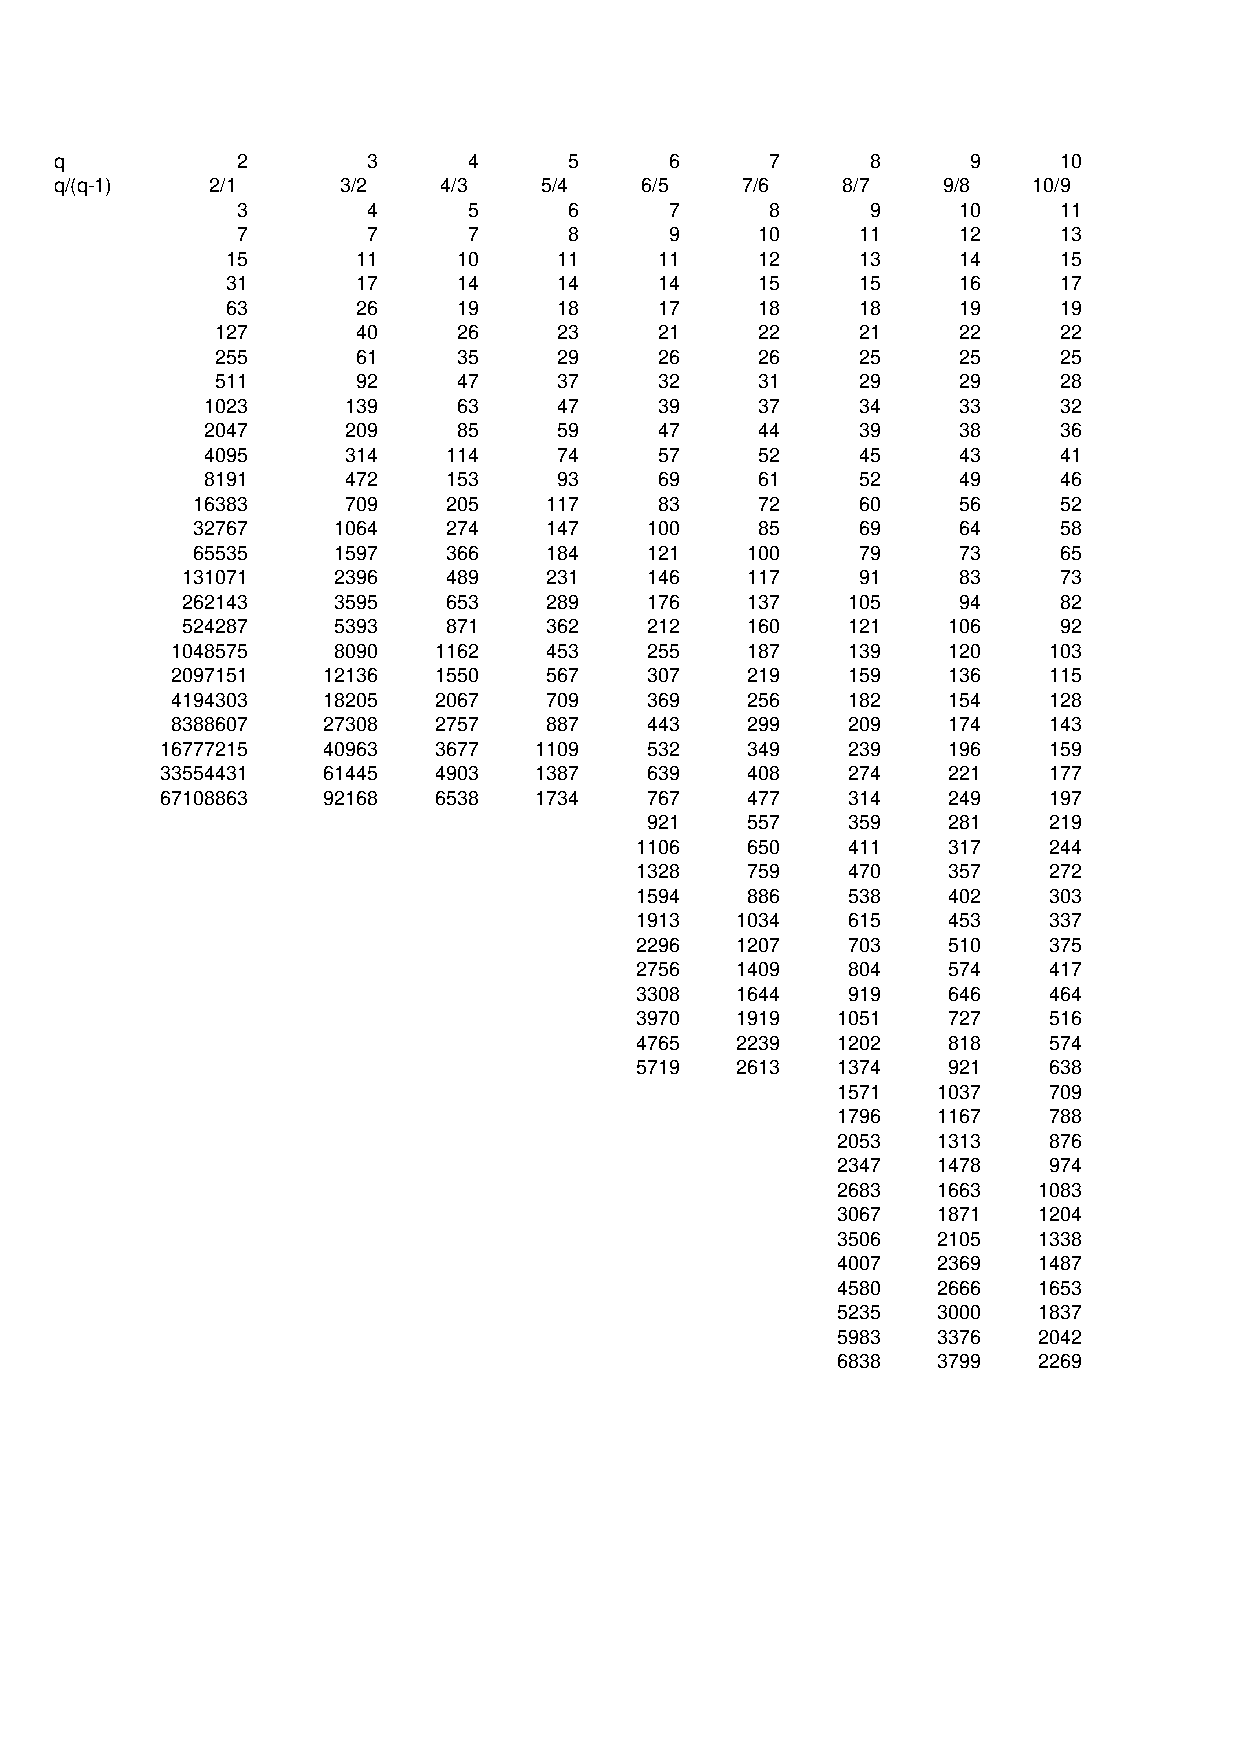
\includegraphics[width=1.0\textwidth]{JosephusTabel}
En sådan tabel er vist her for \(q\) op til \(10\). Hvis for eksempel \(q=5\) og \(n=15\) skal vi finde den største \(d\) således at \(0<nq-d<n\). Vi ser i kolonnen for \(q=5\) og finder at den største \(d\) der er mindre end \(nq=75\) er \(74\). Derfor er overleveren \(75-74=1\).


\end{document}






